% The following choice requires a coordinated choice when PRINTING the report:
%\documentclass[oneside,12pt]{report}  % Use this for one-sided copying (print with printer's normal
%  single-sided option
\documentclass[twoside,12pt,openright]{report}  % You can use this for a slim final printed copy (print with 
%  printer's double-sided option)

% the dimensions of the page
\textheight=9.25in \topmargin=-0.5in   %See note in Chapter 8 of Sample Report about "Pxage scaling" option in Adobe
\textwidth=6.0in
\oddsidemargin=0.3in
\evensidemargin=0.3in  % Needed to balance even and odd pages in twoside print copy

% Useful packages
\usepackage{amsmath}
\usepackage{amsfonts}
\usepackage{url}

%% In the following, the assumption is that your graphics are in encapsulated postscript (eps).  If not,
%% you may need to use some other method for incorporating graphics into your pdf of the final report.
%  Use the next package for typesetting directly to dvi or postcript (used primarily for the PCTeX typesetter, 
%  see the following alternatives).
\usepackage[dvips]{graphicx} 
% Use the next two packages together for typesetting directly to pdf (this works for pdfLaTeX and may work 
% for others---not yet tested for all---please report your experience).
%\usepackage[pdftex]{graphicx}
%\usepackage{epstopdf}
%%

\usepackage{doc}
% Following sets up logic and formatting for conditional twoside copying
\usepackage{ifthen, color, fancyvrb}
\usepackage{wasysym}
\usepackage{marvosym}
\usepackage{nextpage}\pagestyle{plain}
\newcommand\myclearpage{\cleartooddpage
  [\thispagestyle{empty}]
  }

%  Set font size for captions
\usepackage[skip=4pt,font=footnotesize]{caption}


\DeclareGraphicsExtensions{ps,eps}
\usepackage{excludeonly}

% If some words are being hyphenated incorrectly, they can be
% given in a list to the \hyphenation command as below.
\hyphenation{ap-pen-dix wer-ther-i-an}

% Theorem-like command definitions:
\newtheorem{theorem}{Theorem}[chapter]
\newtheorem{lemma}{Lemma}[chapter]
\newtheorem{definition}{Definition}  % Note, this italicizes everything

% Print the chapter and sections in the toc
\setcounter{tocdepth}{1}

\DeclareMathOperator*{\argmin}{arg\,min}
\DeclareMathOperator*{\argmax}{arg\,max}

% Specify which files to typeset for this run (note that overall pagination is preserved)
%\includeonly{chapter1, chapter2}

% Specify which files NOT to typeset for this run (note that overall pagination is preserved)
%\excludeonly{}

% Groundwork for allowing double-sided copying with blank versos
\def\prefacesection#1{
\chapter*{#1}
\addcontentsline{toc}{chapter}{#1}
}

\begin{document}

% Footnote references are symbolized in the front matter, but see below for restoration of numbered footnotes in the body.
\def\thefootnote{\fnsymbol{footnote}}

% The title page is in its own file, ``titlepage.tex''.
% It needs to be edited to reflect information specific
% to your project. 
% don't display the page number
\thispagestyle{empty}

% The numbers below controls the amount of space between the following sections
\def\shiftdowna{0.32in}  % Adjust for balance
\def\shiftdownb{0.22in}  % Adjust for balance

% Set up the boiler plate at the top of the page

\begin{center}
\textbf{{\large Undergraduate Applied Math Research Project at UCSB}}\\

\vspace \shiftdowna
%\includegraphics[width=0.4\textwidth]{ipam.eps}\\
%\includegraphics[width=0.4\textwidth]%{Graphics/ipamlogo_cmyk_full_lg.eps}\\

% SPONSOR
\vspace \shiftdowna
\underline {Sponsor}\\ 
\vspace{5pt}
\textbf{{\large UCSB \& HKUST}}\\
\vspace \shiftdowna
\textbf{Final Report}

% TITLE
\vspace \shiftdowna
\textbf{\Large Localization of eigenstates in 1D physical models: \\A numerical approach to ordered and disordered systems}

% Note the convention used here:  email addresses and urls are typeset in teletype font, colleges are set in italics.

% STUDENTS
\vspace{0.35in}
\underline {Participant}\\
\vspace{5pt}
\text{Xiaofeng Xu} , \text{\emph{Hong Kong University of Science and Technology}}\\ 
\vspace{3pt}
\texttt{\Letter \,\,xxuam@connect.ust.hk}\\
\vspace{5pt}

% SUPERVISOR
\vspace \shiftdownb
\underline {Supervisor} \\
\vspace{5pt}
\text{Prof. Carlos García-Cervera}, \text{\emph{University of California, Santa Barbara}}\\ 

% SPONSORS
%\vspace \shiftdownb
%\underline {Sponsoring Mentors}\\
%\vspace{5pt}
%Zhixiong Long\\
%\vspace{3pt}
%Sean Yu

% CONSTULANTS (comment out this text if there are no consultants)
%\vspace \shiftdownb
%\underline {Consultants}\\
%\vspace{5pt}
%$\langle \text{Name}\rangle$\\
%\vspace{3pt}
%$\langle \text{Name}\rangle$

% DATE
\vspace \shiftdowna
August 31st, 2018

\end{center}

%\vfill  %Fill page to force following note to bottom
%\footnoterule
%\noindent \small{This project was jointly supported by IPAM, HKUST, FitME, XiaofuTech, Dr. Lee Shiu and Dr. Jennie Mui Lee, and NSF Grant DMS-1440415.}



% Begin ABSTRACT
\ifthenelse{\boolean{@twoside}}{\myclearpage}{}
\prefacesection{Abstract}
% don't display the page number
%\thispagestyle{empty}


Physicists have been very interested in transport phenomena in disordered systems like crystals with impurities. The feature of eigenstates is of great importance for understanding transport phenomena in such systems. Hence, a numerical approach using finite difference method is used to solve one dimensional Schr\"{o}dinger equations for ordered and disordered systems. Comparisons are made in order to reveal a fundamental difference, namely localization properties, between these two systems. We explore other factors like potential height, atomic spacing to see their effect on degree of localization in our modified random Kronig Penney model that we will introduce in this paper. Moreover, another model in which we consider a chain of atoms connected by strings obeying Hooke's law is also explored with some randomness that we introduce. In their normal modes, we again find localization properties for these systems. To some extent, this indicates localization is a universal property for disordered systems. Finally, with the aid of finite difference method and Bloch theorem, we explore band structure for periodic Kronig Penney models with negative finite potential wells. In particular, we look at band gaps of these models and explore its relation with the periodic potential. 

% Begin ACKNOWLEDGMENTS
\ifthenelse{\boolean{@twoside}}{\myclearpage}{}
\prefacesection{Acknowledgments}
The research was carried out during my exchange study at University of California Santa Barbara and the research project was generously funded by the School of Science at Hong Kong University of Science and Technology. I am very grateful to HKUST and UCSB for providing me with this exchange opportunity, without which the research project would not be possible. 

I especially would like to thank my supervisor Prof. Carlos García-Cervera for giving me this research opportunity as well as his invaluable advice and guidance in helping me formulate this project. Not only did I obtain much insight into the topic, but I also had a good time talking and discussing problems with him as well as developed great interest in quantum mechanics. He was always available to answer many questions as well as give me constructive suggestions and ideas towards the success of this project. Throughout the whole project period, I truly appreciate the time he took to have regular meetings with me, during which he patiently listened to my presentations and corrected any mistakes that I made. I would like to express my sincerest gratitude to Prof. Carlos García-Cervera for his help, guidance, and support. 

I would also like to thank my friend, Wei Ren, who has been studying and discussing physics related to my research with me for the whole summer. I truly enjoyed working, talking and exploring new topics with Wei. 

% Table of contents, List of Figures, and List of Tables.
\ifthenelse{\boolean{@twoside}}{\myclearpage}{}
\tableofcontents

\ifthenelse{\boolean{@twoside}}{\myclearpage}{}
\listoffigures

\ifthenelse{\boolean{@twoside}}{\myclearpage}{}
\listoftables

% The report is an extensive document.
% It is convenient to have each chapter of the report in its own file
% rather than throw all work together in a single file.
% Do not run the LaTeX typesetter on each individual chapter; refresh
% your report by running the typesetter on this master file.

% Cancel the previous symbol requirement for footnotes in the front
% matter, and use arabic numerals for footnotes in the body
\renewcommand{\thefootnote}{\arabic{footnote}}
\setcounter{footnote}{0}

% Chapter 1 -- the Introduction
\ifthenelse{\boolean{@twoside}}{\myclearpage}{}
\chapter{Introduction}\label{Ch:Introduction}

Properties of ordered system like regular crystals have been well studied and understood by physicists. A distinct feature about regular crystal is the occurrence of band gap, which is well demonstrated in the Kronig Penney model \cite{kronigPenneyModel}. A detailed numerical study will be carried out in this paper to further explore band gap in Kronig Penney models.We also modify these models to get a one-dimensional disordered systems and study the differences between ordered systems and disordered systems.


Both numerical and theoretical results regarding disordered systems had also already been obtained by physicists\cite{summerPaper}. However, in this paper, we mainly focus on the numerical parts that have been studied previously\cite{summerPaper}, but with the advancement of computational abilities and modern algorithms, we explore these properties through a different approach and in more details. 

%\begin{figure}[ht]
%\centering
%\includegraphics[scale=1]{Graphics/flowchart.png}
%\caption{Project Flowchart}
%\label{fig:flowchart}
%\end{figure}

\section{Project Goal}
We explore finite difference method \cite{finiteDifferenceMethod} for solving one-dimensional Schr\"{o}dinger equation with different boundary conditions. We utilize the eigenvalue solver to get the eigenvalues and eigenstates for different one-electron systems, namely regular systems with periodic potential and disordered system with some randomness that we introduce. Not only do we need to obtain the solutions under different systems, but we are also hoping to reveal some relation between different quantities in these systems, and develop some intuition for major differences between ordered and disordered one dimensional systems. Our ultimate goal will be to come up with an analytic reasoning behind these rules that we observed in our numerical experiments so that they can serve as guiding physical principles in certain situations. 



\section{Organization}

The paper is organized as follows. In Chapter 2, we explain the models and corresponding physical quantities that we are studying in this paper.We also give a brief introduction to mathematical equations governing each model.  In Chapter 3, we describe our finite difference scheme for solving these equations and convert each problem into an eigenvalue problem of finite dimensions. We will also introduce the major programming tools that we used for solving these eigenvalue problems. In Chapter 4, we present our results for each model from our numerical experiments. Findings, some conclusions, and possible future exploration directions will be discussed in Chapter 5. Our core working codes are too lengthy to be included in this paper but can be requested through email.  
\endinput


% Chapter 2
\ifthenelse{\boolean{@twoside}}{\myclearpage}{}
\chapter{Background}\label{Ch:Background}
In this chapter, we introduce the models that we study in this paper, both ordered and disordered systems. For disordered systems, we will explain how we introduce randomness into the system. 



\section{Model 1}\label{model:model1}
\subsection{model 1a}

The model we are studying is represented by the one-dimensional time-independent Schrodinger equation: 
\begin{equation} \label{eq:2.1}
-\frac{d^2\psi}{dx^2}+V(x)\psi=E\psi
\end{equation}
where the potential consist of non-overlapping atomic potential similar to the Kronig Penny model. But we use finite negative square well potential instead of delta potential at each atom site (See the figure below).

Also, for this model we impose zero boundary conditions for the wave function. This means the potential is positive infinity at two ends. 

\begin{figure}[h]
\centering
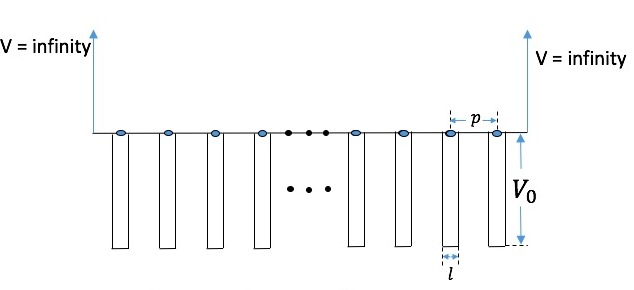
\includegraphics[scale=0.75]{Graphics/square_potential_problem.jpeg}
\caption{Model1a, $p$, $l$, $V_0$ denotes atom spacing, square well width, and potential height respectively}
\label{fig:net}
\end{figure}

\newpage
\subsection{model 1b}
Model 1b is derived from model 1a by introducing some randomness to atomic spacing to a chain of atoms. With potential height($V_0$) and well width($l$) fixed, the atomic spacing between any two atoms now takes two values from ${\{p_1,p_2\}}$ with probability ${\{P(p_1),P(p_2)\}}$. The boundary conditions are the same as in model 1a.
\subsection{model 1c}
In model 1c, randomness is introduced to the potential well at each atom site. This time, both atomic spacing and potential well width  are  fixed, but the potential height at each atom site takes a value from $\{V_1,V_2\}$ with probability $\{P(V_1),P(V_2)\}$. Again, the same boundary condition as in model 1a applies to model 1c. 

\section{Model 2}\label{bloch theorem}
In this model we study a chain of atoms with non-overlapping negative square well potential under periodic boundary conditions. (See figure below).
\begin{figure}[h]
\centering
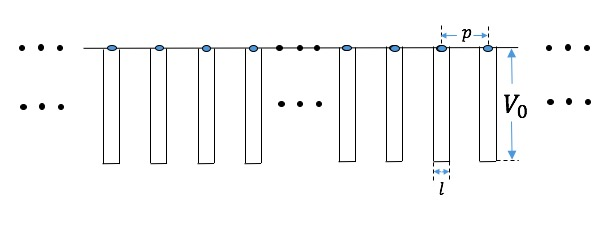
\includegraphics[scale=0.75]{Graphics/kp_bandgap.jpeg}
\caption{Model2}
\label{fig:net}
\end{figure}
The corresponding time-independent Schrodinger equation that governs that system is the same as equation \ref{eq:2.1} but with the potential being periodic with a period $p$, i.e. $V(x) = V(x+p)$ in this case. 
If we consider a sample of N atoms, due to the periodicity, we may impose the Von Karman condition\cite{BoundaryCondition} at the macroscopic boundary,i.e. $\psi(x+Np) = \psi(x)$. 
By use of Bloch theorem \cite{BlochTheorem}, we know that the solution would be of the form $$\psi_k(x) = e^{i{\alpha_k}x}u_k(x),$$ with $u_k(0) = u_k(p)$,
and $\alpha_k$ taking values (Note that $\alpha_k$ is called the wave vector)
$$\alpha_k = \frac{x\pi k}{Np}, \quad k = -\frac{Np}{2},...,\frac{Np}{2}. $$
After substituting it into equation \ref{eq:2.1}, we can get
\begin{equation}\label{eq:2.2bloch}
-\frac{1}{2}(\frac{d}{dx}+i\alpha_k)^2u_k+V(x)u_k = Eu_k
\end{equation}

With the above equation, for each wave vector, we can solve the Schr\"{o}dinger equation and get the corresponding eigenvalues. If we plot the eigenvalues against wave wave vectors. We can obtain a band structure for this one-dimensional periodic system, from which we can determine the band gap, which is the difference of the smallest eigenvalue in the second band and the largest eigenvalue in the first band.

\section{Model 3}
In this model, we consider a chain of $N+1$ atoms connected by harmonic strings, meaning that the interaction between the nearest neighboring atoms obey Hooke's law. The system is shown in the following graph. 
\begin{figure}[h]
\centering
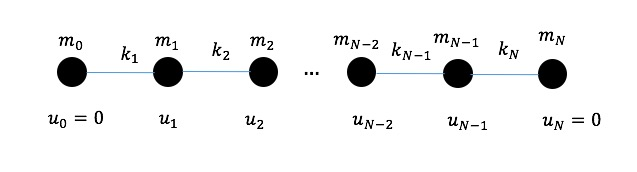
\includegraphics[scale=0.75]{Graphics/harmonicChain.jpeg}
\caption{Model 3:Harmonic chain model}
\label{fig:net}
\end{figure}
As shown in this graph,  $k_n$ is the elastic constant of the harmonic string between the $(n-1)$th and $n$th atom. $u_n$ and $m_n$ are respectively the displacement from its equilibrium position and the mass of the $n$th atom. 
We impose fix-end boundary conditions at both ends of this chain
$$u_0 = u_N = 0.$$
By looking at a certain atom and analyzing the forces on it, the model can be represented by the following equation of motion 
\begin{equation}\label{eq:harmonicChain}
m_n\frac{d^2u_n}{dt^2} = k_n(u_{n+1}-u_n) - k_{n-1}(u_n-u_{n-1}), (n = 1,2,...,N)
\end{equation}
Assuming the monochromatic time dependence $u_n \propto exp(-iwt)$ in Equation \ref{eq:harmonicChain}, we have the following stationary equation of motion \cite{summerPaper}
\begin{equation}\label{eq:timedependence}
-m_nw^2u_n = k_n(u_{n+1}-u_n) - k_{n-1}(u_n-u_{n-1}), (n = 1,2,...,N)
\end{equation}


\subsection{model 3a}
Model 3a assumes that each atom only takes the mass from two values $\{M_1,M_2\}$ with probability ${P(M_1),P(M_2)}$. The strength of the harmonic strings between the nearest neighboring atoms is taken to be 1. In this case, Equation \ref{eq:timedependence} reduces to 
\begin{equation}\label{eq:model 3a}
-m_nw^2u_n = u_{n+1}-2u_n + u_{n-1}, (n = 1,2,...,N). 
\end{equation}

\subsection{model 3b}
Model 3b assumes that all atoms have the same mass, taken to be 1. The strength of the harmonic strings, i.e. the elastic constant,  now takes a value from two values $\{K_1,K_2\}$ with probability $\{P(K_1),P(K_2)\}$. In this case, Equation \ref{eq:timedependence} reduces to 
\begin{equation}\label{eq:timedependence}
-w^2u_n = k_n(u_{n+1}-u_n) - k_{n-1}(u_n-u_{n-1}), (n = 1,2,...,N)
\end{equation}
where $k_n$, $k_{n-1}$ is is either $K_1$ or $K_2$ respectively. 



\endinput


% Chapter 3
\ifthenelse{\boolean{@twoside}}{\myclearpage}{}
\chapter{Methodology}\label{Ch:Methodology}



\section{Finite Difference Scheme for differential operator}
In order to solve the Schr\"{o}dinger equation \ref{eq:2.1} in Chapter \ref{Ch:Background}, we apply the finite difference method to approximate the second derivative and convert this problem into a finite-dimensional eigenvalue problem, represented by a matrix. 
Equation \ref{eq:2.2bloch} in Model 2 involves both a second derivate and a first derivative, hence in this case, we apply the finite difference method to approximate both. 


\subsection{}
In this subsection, We focus on convert the following Schr\"{o}dinger equation into a matrix form under the centered finite difference approximation.  
\begin{equation} \label{eq:3.1}
-\frac{d^2\psi}{dx^2}+V(x)\psi=E\psi
\end{equation}

In a general setting, we solve the 1D Schr\"{o}dinger equation in the interval $[a,b]$, with $b > a$ and we impose the zero boundary condition for wave function, meaning that $\psi(a) = \psi(b) = 0$. 
We first discretize the continuous interval into a sequence of equally spaced points$\{x_n\}_{n = 0,1,...,N}$,where $x_0 = a$ and $x_N = b$. We denote by h the spacing between the points, i.e. discretization accuracy. Since the Schr\"{o}dinger equation holds at each point. 
We have the following equations approximating the system: 
\begin{align*} \label{eq:2}
 -\frac{d^2\psi(x_1)}{dx^2}+V(x_1)\psi(x_1)&= E\psi(x_1)  \\ 
-\frac{d^2\psi(x_2)}{dx^2}+V(x_2)\psi(x_2)&= E\psi(x_2) \\
...\\
-\frac{d^2\psi(x_{N-2})}{dx^2}+V(x_{N-2})\psi(x_{N-2})&= E\psi(x_2)\\
-\frac{d^2\psi(x_{N-1})}{dx^2}+V(x_{N-1})\psi(x_{N-1})&= E\psi(x_{N-1})\\
\end{align*}
Note that at point $x_0$ and $x_N$, the value of the wave function is already known by the boundary condition. 
Then, we use the centered finite difference method to approximate all the second derivatives. 
\begin{equation} \label{eq:3}
\frac{d^2\psi(x_i)}{dx^2} \approx \frac{\psi(x_{i-1})-2\psi(x_i)+\psi(x_{i+1}))}{2h^2}
\end{equation}
Thus by substituting the second derivatives and considering the boundary conditions, the previous equations can be rewritten as the following:
\begin{align*} \label{eq:2}
 -\frac{-2\psi(x_1)+\psi(x_{2})}{2h^2}+V(x_1)\psi(x_1)&= E\psi(x_1)  \\ 
-\frac{\psi(x_{1})-2\psi(x_2)+\psi(x_{3})}{2h^2}+V(x_2)\psi(x_2)&= E\psi(x_{2}) \\
...\\
-\frac{\psi(x_{N-3})-2\psi(x_{N-2})+\psi(x_{N-1})}{2h^2}+V(x_{N-2})\psi(x_{N-2})&= E\psi(x_{N-2})\\
-\frac{\psi(x_{N-2})-2\psi(x_{N-1})}{2h^2}+V(x_{N-1})\psi(x_{N-1})&= E\psi(x_{N-1})\\
\end{align*}

For convenience, we denote $\psi(x_i)$ as $\psi_i$, $V(x_i)$ as $V_i$. We can then write the preceding equations in the following matrix form: 

\begin{equation} \label{eq:matrix1}
\left[ \begin{matrix}
\frac{1}{h^2}+V_1 & -\frac{1}{2h^2} & & 0\\
-\frac{1}{2h^2} & \ddots & \ddots & \\
& \ddots & \ddots & -\frac{1}{2h^2} \\
0 & & -\frac{1}{2h^2} & \frac{1}{h^2}+V_{N-1} \end{matrix} \right]
\begin{bmatrix}
    \psi_{1}  \\
    \psi_{2}  \\
    \vdots  \\
    \psi_{N-2}\\
    \psi_{N-1}
    \end{bmatrix} = E\begin{bmatrix}
    \psi_{1}  \\
    \psi_{2}  \\
    \vdots  \\
    \psi_{N-2}\\
    \psi_{N-1}
    \end{bmatrix}
\end{equation}

From the matrix representation of the Schr\"{o}dinger equation, we can easily see that the discretized wave function is a eigenvector of the matrix corresponding to the eigenvalue $E$. Hence, in order to get the wave function and its energy for such a system, we can compute the eigenvalues and eigenvectors for this matrix. 

In order to study localization properties of wave function, we compute the probability density function from the eigenvectors. Notice that the eigenvectors may not be an exact wave function. We need to properly rescale the eigenvector to obtain the wave function and then the probability density function. 
From the probability density function, we can then compute the variance to measure the degree of localization of a wave function. 

\subsection{}
In this subsection, we convert the equation \ref{eq:2.2bloch} in Chapter \ref{Ch:Background} to its matrix form using centered finite difference method similar to the preceding subsection. 
We first expand the bracket in equation \ref{eq:2.2bloch} and we get the following: 
\begin{equation}\label{eq:expand}
-\frac{1}{2}\frac{d^2u_k}{dx^2}-i\alpha_k \frac{d u_k}{dx} +\frac{1}{2}{\alpha_k}^2u_k+V(x)u_k = Eu_k
\end{equation}
We discretize the interval for this problem into a sequence of equally spaced points $\{x_n\}_{n = 0,1,...,N}$ with discretization accuracy $h$. Because the above equation \ref{eq:expand} holds at all these points, we have the following equations:
\begin{align*} 
 -\frac{1}{2}\frac{d^2u_k(x_0)}{dx^2}-i\alpha_k \frac{d u_k(x_0)}{dx} +\frac{1}{2}{\alpha_k}^2u_k(x_0)+V(x_0)u_k(x_0)  &= Eu_k(x_0)  \\
  -\frac{1}{2}\frac{d^2u_k(x_1)}{dx^2}-i\alpha_k \frac{d u_k(x_1)}{dx} +\frac{1}{2}{\alpha_k}^2u_k(x_1)+V(x_1)u_k(x_1)  &= Eu_k(x_1) \\
......\\
 -\frac{1}{2}\frac{d^2u_k(x_N)}{dx^2}-i\alpha_k \frac{d u_k(x_N)}{dx} +\frac{1}{2}{\alpha_k}^2u_k(x_N)+V(x_N)u_k(x_N)  &= Eu_k(x_N) \\
\end{align*}

Then, we use the centered finite difference method to approximate both the second derivative and first derivative. For convenience, we drop the subscript $k$. 

\begin{align*} 
\frac{d^2u(x_i)}{dx^2} & \approx \frac{u(x_{i-1})-2u(x_i)+u(x_{i+1}))}{2h^2} \\
\frac{du(x_i)}{dx} & \approx \frac{u(x_{i+1})-u(x_{i-1})}{2h}
\end{align*}
We plug in the above two approximations and apply the periodic boundary condition. After rearranging, we get the following: 
\begin{equation} \label{eq:dis_periodic}
(-\frac{1}{2h^2}+\frac{i\alpha}{2h})u_{i-1} + (\frac{1}{h^2}+\frac{1}{2}\alpha^2+V_i)u_i+(-\frac{1}{2h^2}-\frac{i\alpha}{2h})u_{i+1} = Eu_i  
\end{equation}
Note that the periodic boundary condition that we impose imply that at $x_0$, $u_{-1}$ would be $u_{N}$. Similarly, at $x_N$, $u_{N+1}$ would be $u_{0}$. 
Hence, we can convert the system into its matrix form as follows. Note that except the main diagonal and the diagonals above and below it, all other unfilled entries are zeros. 
\begin{equation} \label{eq:matrix2}
\left[ \begin{matrix}
\frac{1}{h^2}+\frac{1}{2}\alpha+V_0 & -\frac{1}{2h^2}-\frac{i\alpha}{2h} & & -\frac{1}{2h^2}+\frac{i\alpha}{2h}\\
-\frac{1}{2h^2}+\frac{i\alpha}{2h} & \ddots & \ddots & \\
& \ddots & \ddots & -\frac{1}{2h^2}-\frac{i\alpha}{2h} \\
-\frac{1}{2h^2}-\frac{i\alpha}{2h} & & -\frac{1}{2h^2}+\frac{i\alpha}{2h} & \frac{1}{h^2}+\frac{1}{2}\alpha+V_{N} \end{matrix} \right]
\begin{bmatrix}
    u_{0}  \\
    u_{1}  \\
    \vdots  \\
    u_{N-1}\\
    u_{N}
    \end{bmatrix} = E\begin{bmatrix}
    u_{0}  \\
    u_{1}  \\
    \vdots  \\
    u_{N-1}\\
    u_{N}
    \end{bmatrix}
\end{equation}


\section{Matrix form of the harmonic chain model}
For easy illustration of the matrix in model 3a and model 3b, we analyze the matrix form of the model when all the masses are of unit 1 and the strength of the harmonic string is taken to be 1 as well. So equation \ref{eq:timedependence} becomes
\begin{equation}\label{eq:model3 regular}
-w^2u_n = u_{n+1}-2u_n +u_{n-1}, (n = 1,2,...,N). 
\end{equation}
By collecting these equations for $n=1,2,...N-1$ and put them into matrix form, we have the following:

\begin{equation} \label{eq: matrix regular}
\left[ \begin{matrix}
2 & -1 & & 0\\
-1 & \ddots & \ddots & \\
& \ddots & \ddots & -1 \\
0 & & -1 & 2 \end{matrix} \right]
\begin{bmatrix}
     u_{1}  \\
     u_{2}  \\
    \vdots  \\
    u_{N-2}\\
    u_{N-1}
    \end{bmatrix} = w^2\begin{bmatrix}
    u_{1}  \\
    u_{2}  \\
    \vdots  \\
    u_{N-2}\\
    u_{N-1}
    \end{bmatrix}
\end{equation}
From the above matrix equation, $w^2$ is the eigenvalue of the matrix and $[u_1,u_2,...,u_{N-1}]^T$ is the eigenvector of it. Hence we can solve for the normal modes(i.e. the eigenstate) by simply solving the matrix for the eigenvalues and eigenvectors. 

For model 3a, the only difference is that we no longer have a unit mass for each atom, this can be reflected on the matrix by dividing the corresponding row of the matrix in \ref{eq: matrix regular} by the mass. Given a chain of atoms with different masses, we can create the matrix for this system and solve for the eigenvalues and eigenvectors. 
For model 3b, all masses are taken to be 1. We can similarly create the matrix for such a system depending on the strength of the harmonic strings. 

\section{Python eigenvalue solver}
In this project, we implement all the models using the NumPy libraries of python. NumPy is a powerful package for scientific computing that allows us to use N-dimensional array objects and provides us with linear algebra capabilities. In particular, we use the eigenvalue solver function numpy.linalg.eig which returns all the eigenvalues and corresponding eigenvectors for a square matrix. For sparse and Hermitian matrices, we also use the function scipy.sparse.linalg.eigs, which offers us more flexibility to decide how many eigenvalues and in what order we want them to be returned. 

% \section{Control variables}
% We introduce randomness into our system using the way we mentioned in Model1 and Model 3  and explore the localization of eigenstates of such disordered systems. We generate several different random chain of atoms to see if localization indeed exist. Then we control variables to explore relation between degree of localization and some factors, namely potential height at each atoms sites, atomic spacings. 
% \subsection{Randomness in atomic spacing}
% After showing localization property of eigenstates, we want to further understand what factors affect it. 

% \subsection{2}
% \subsection{3}
% \subsection{4}
 \endinput


% Chapter 4
\ifthenelse{\boolean{@twoside}}{\myclearpage}{}
\chapter{Results}\label{Ch:Results}

\section{Band gaps in the Kronig Penney Model}

We are interested in how size of a square potential would affect the band gap for such a system. Due to computational limitation, we only consider finite system with periodic boundary conditions, i.e. each atom has the same square well potential as shown below.
We first see whether the number of atoms will affect the band gap. Ideally, if the model is good, there should not be any discrepancies in the band gaps because in each case we are imposing the periodic boundary conditions, so the band gap should be independent of the number atoms we choose. 
\begin{table}[h]
\centering
\begin{tabular}{ c|c|c|c|c|c|c|c } 
 Number of atoms & 11 & 15 & 19& 31 & 51 & 71& 101 \\ 
 \hline
 Band gap & 5.749 & 5.749 & 5.749& 5.749 & 5.749 & 5.749& 5.749\\ 
\end{tabular}
\caption{band gap against number of atoms}
\label{tab:num of atoms vs band gap}
\centering
\end{table}

\newpage
We investigate the behavior of band gap when fixing the well width and varying the potential. 

\begin{figure}[h]
\centering
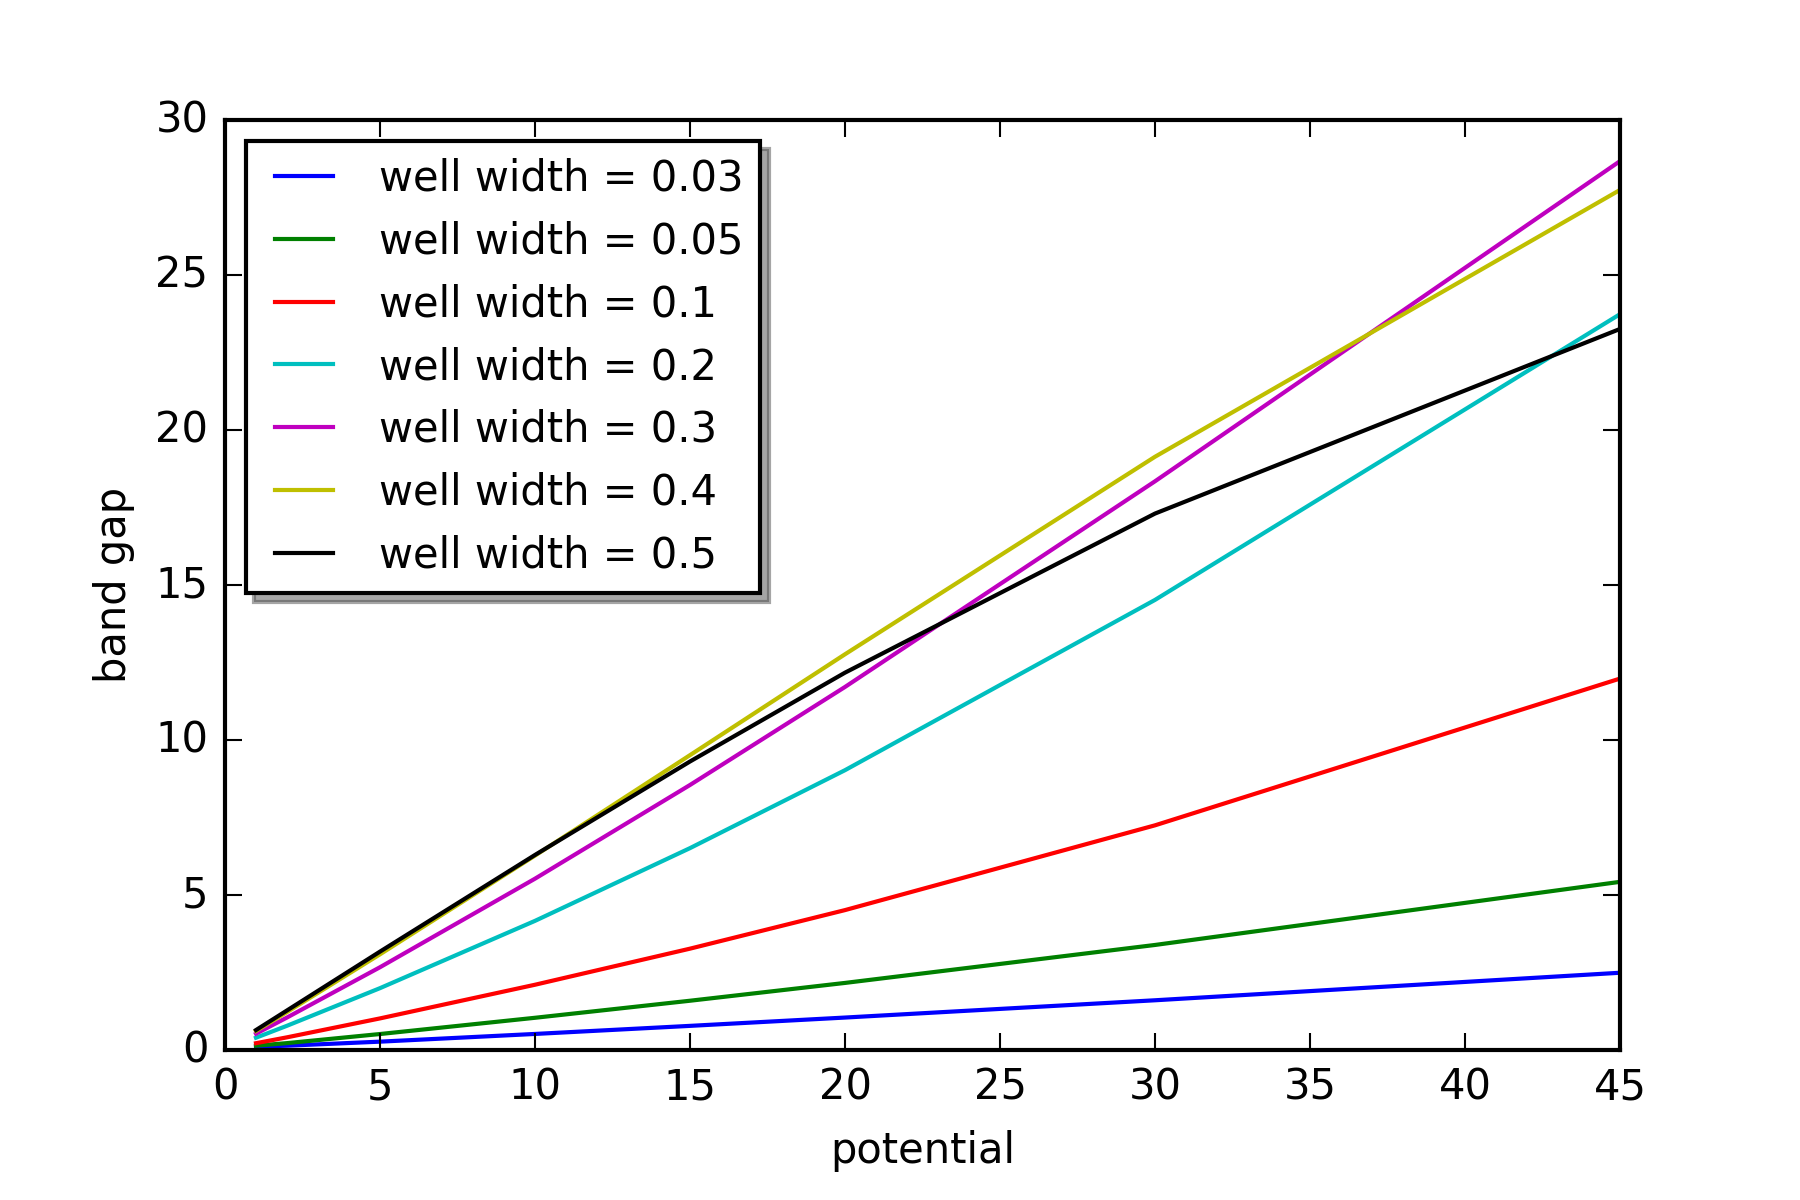
\includegraphics[scale=.8]{Bandgap/30_change_Potentials.png}
\caption{band gap against potential heights at fixed well widths}
\label{fig: band gap against potential }
\end{figure}

We investigate the behavior of band gap when fixing the potential height and varying the well width. 

\begin{figure}[h]
\centering
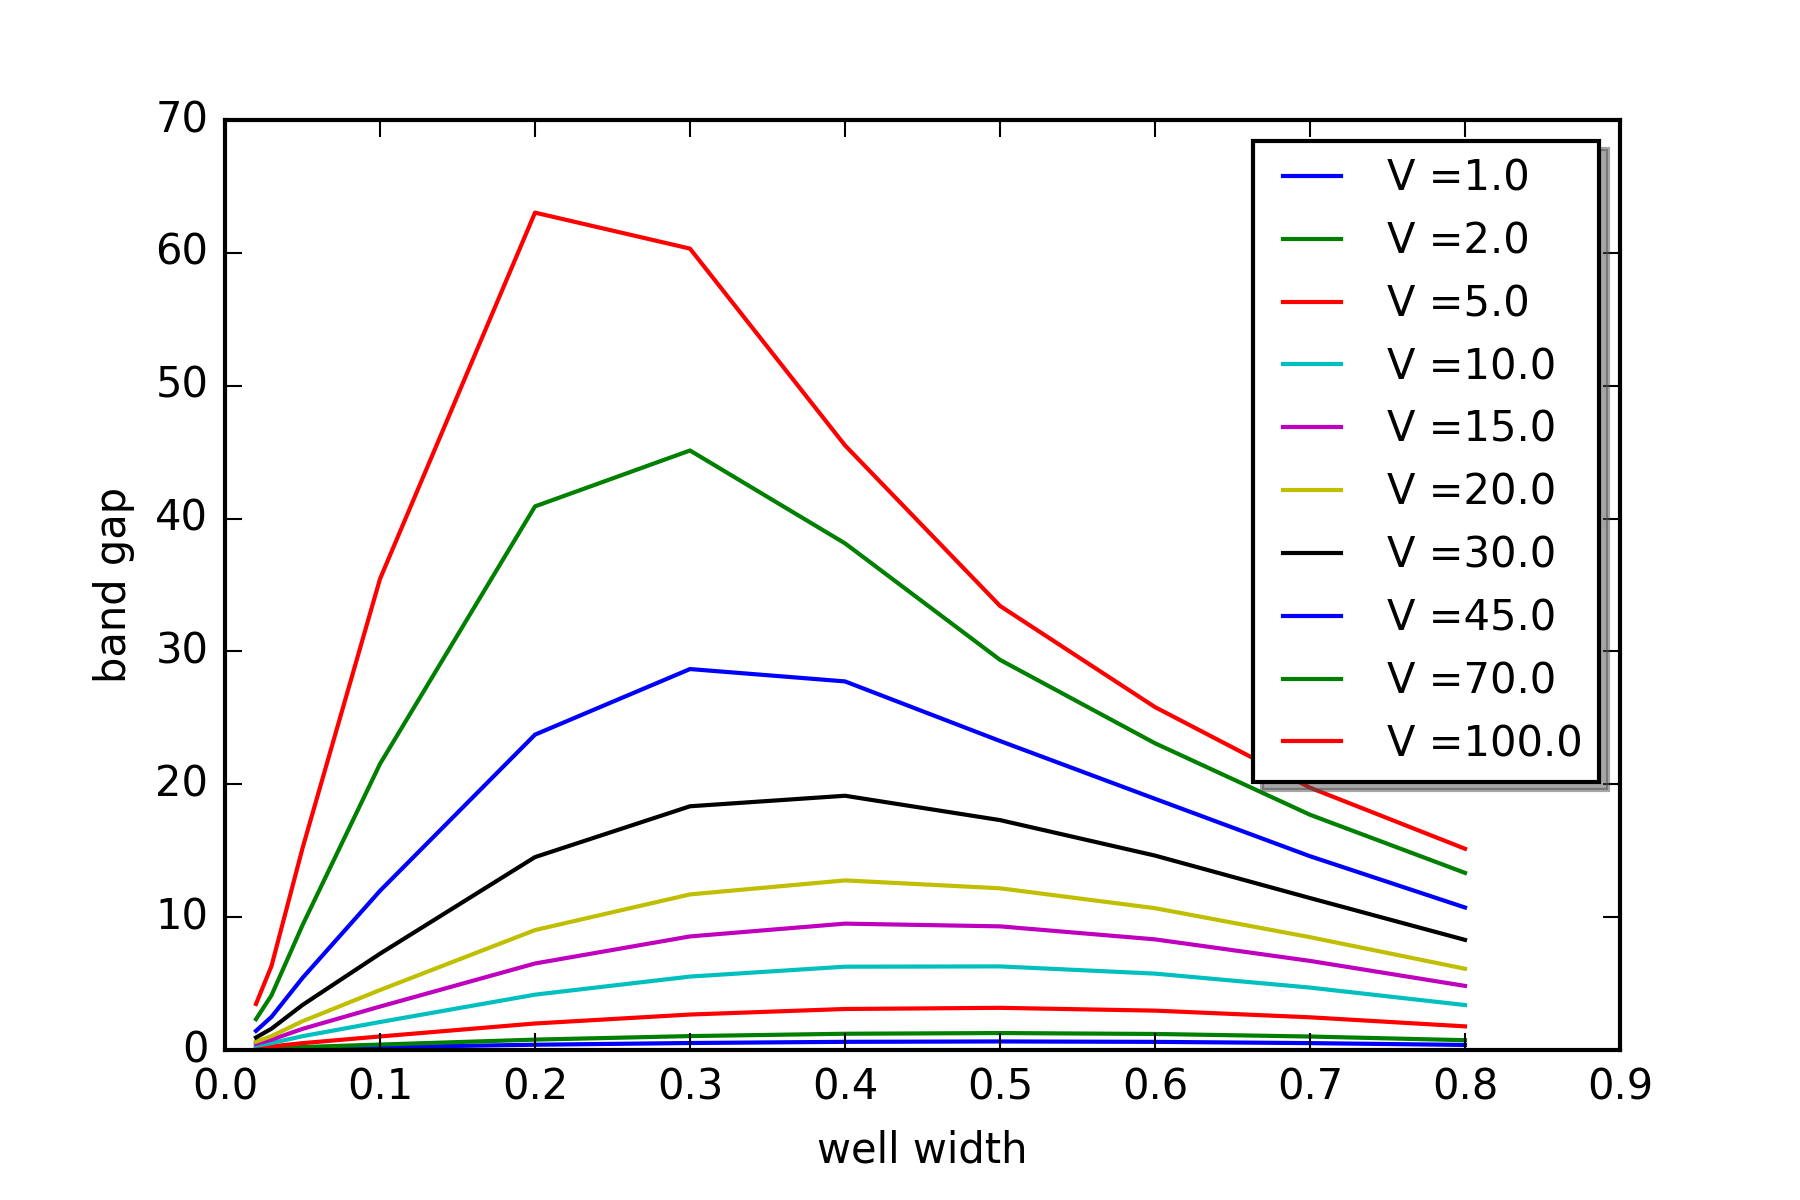
\includegraphics[scale=.8]{Bandgap/complete_change_well_width.png}
\caption{band gap against well width at fixed potentials}
\label{fig:band gap against well width fixed potential}
\end{figure}
\newpage 
Finally, we plot the graph of behavior of band gap when fixing the area of the potential and varying the well width.

\begin{figure}[h]
\centering
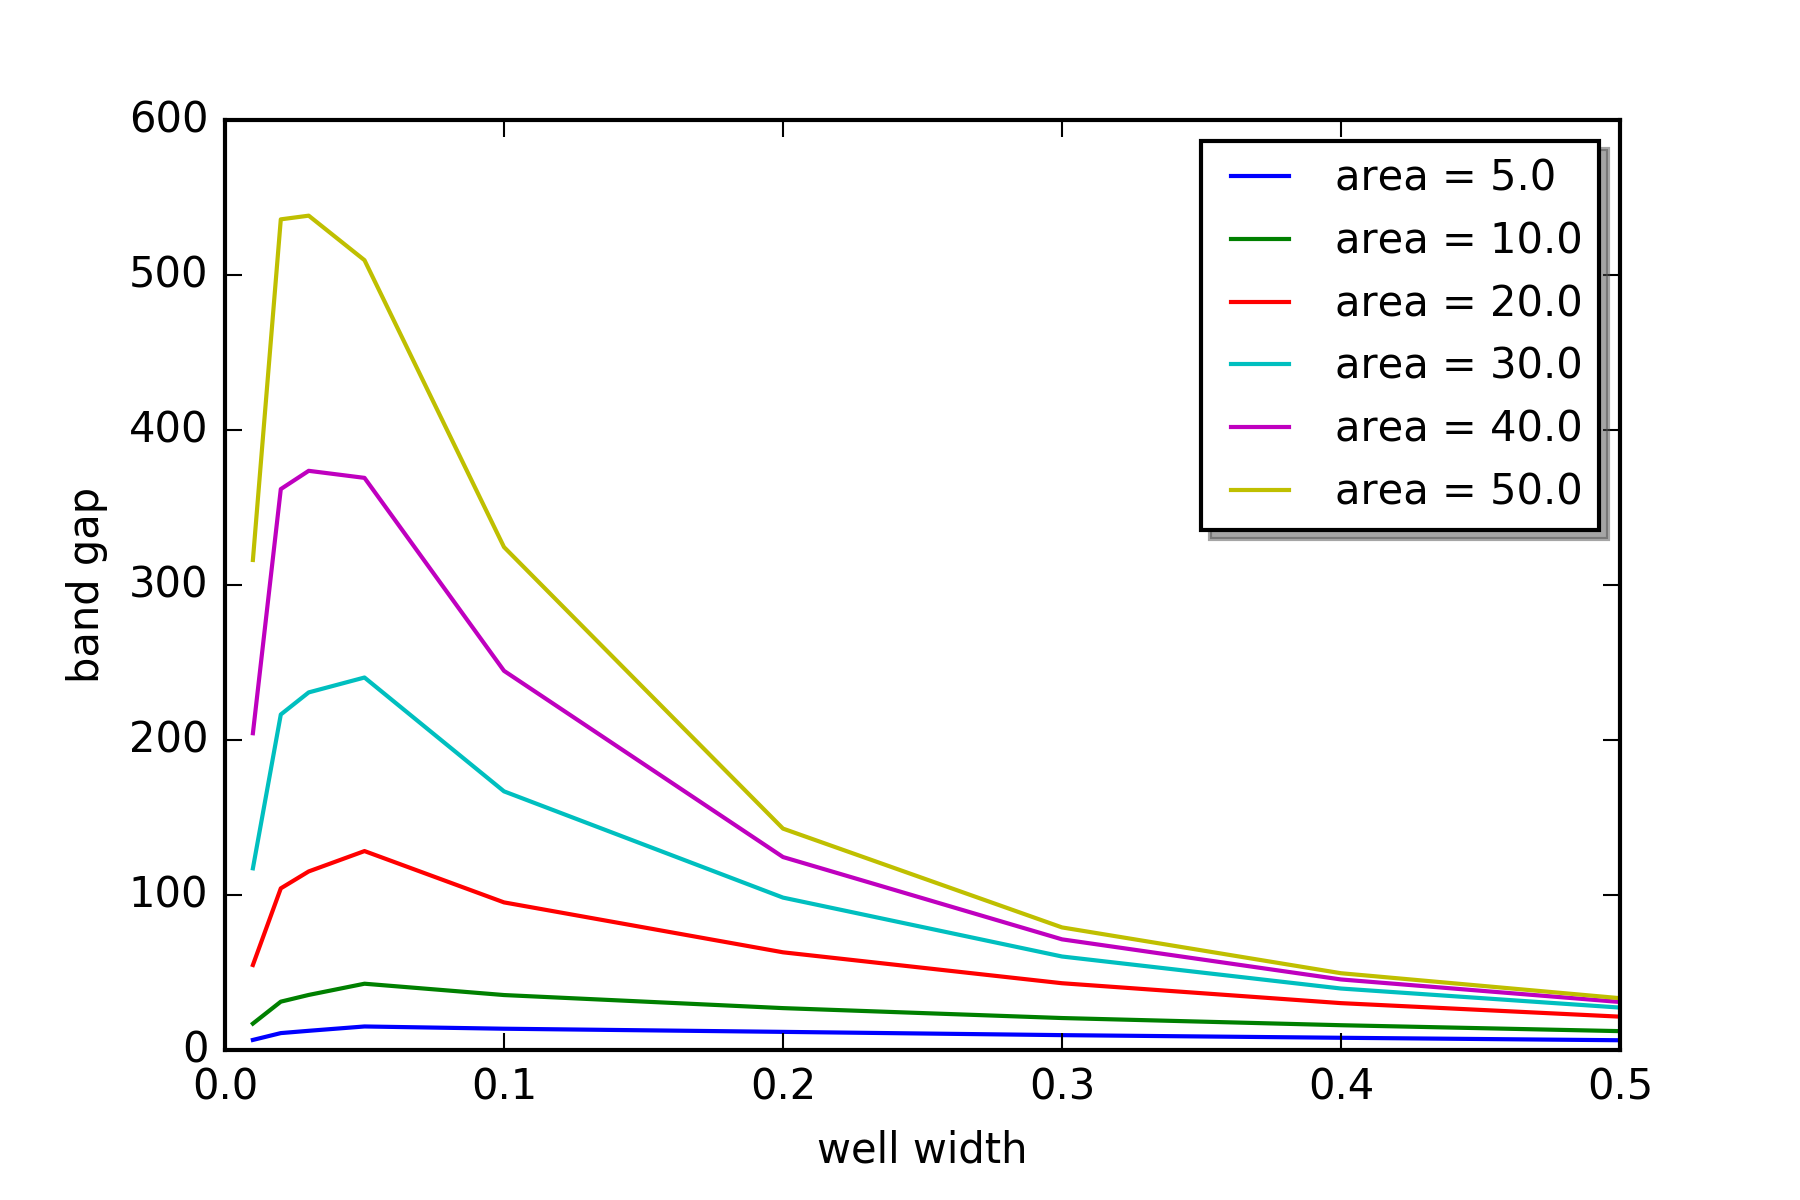
\includegraphics[scale=.8]{Bandgap/change_area5_to_50.png}
\caption{band gap against well width with potential area fixed}
\label{fig:bang gap against well width fixed area}
\end{figure}



\newpage
\section{Localization of eigenstates of Random Kronig Penney Model with zero boundary condition}\label{sec: localization}
In this section, the following figures are for the model we introduced in Chapter \ref{Ch:Background} Section \ref{model:model1}, in which the potential at the boundaries are assumed to be positive infinity, in other words, the wave function at the boundaries is zero.

\subsection{Randomness in atomic spacing}\label{subsec:Randomness in atomic spacing}
The following graphs are the probability density function for both ordered and disordered system under different conditions. The model uses a chain of 31 atoms. The well width is set to be 0.5 for all cases since we are only investigating effect of random spacing between atoms. 

For the ordered system, atoms are equally spaced with 1.0 unit distance.
For the disordered system, the atom spacings are generated from two values$\{p_1,p_2\}$, each with probability 0.5. Then we determine the atom coordinates according to the generated spacings. 

The following are figures for eigenstates of the disordered system when $V_0l$ is equal to 1.
The eigenvalues labeled on each figure are that of an ordered system. 


\begin{figure}[!htbh]
\centering
\begin{minipage}{.45\textwidth}
  \centering
  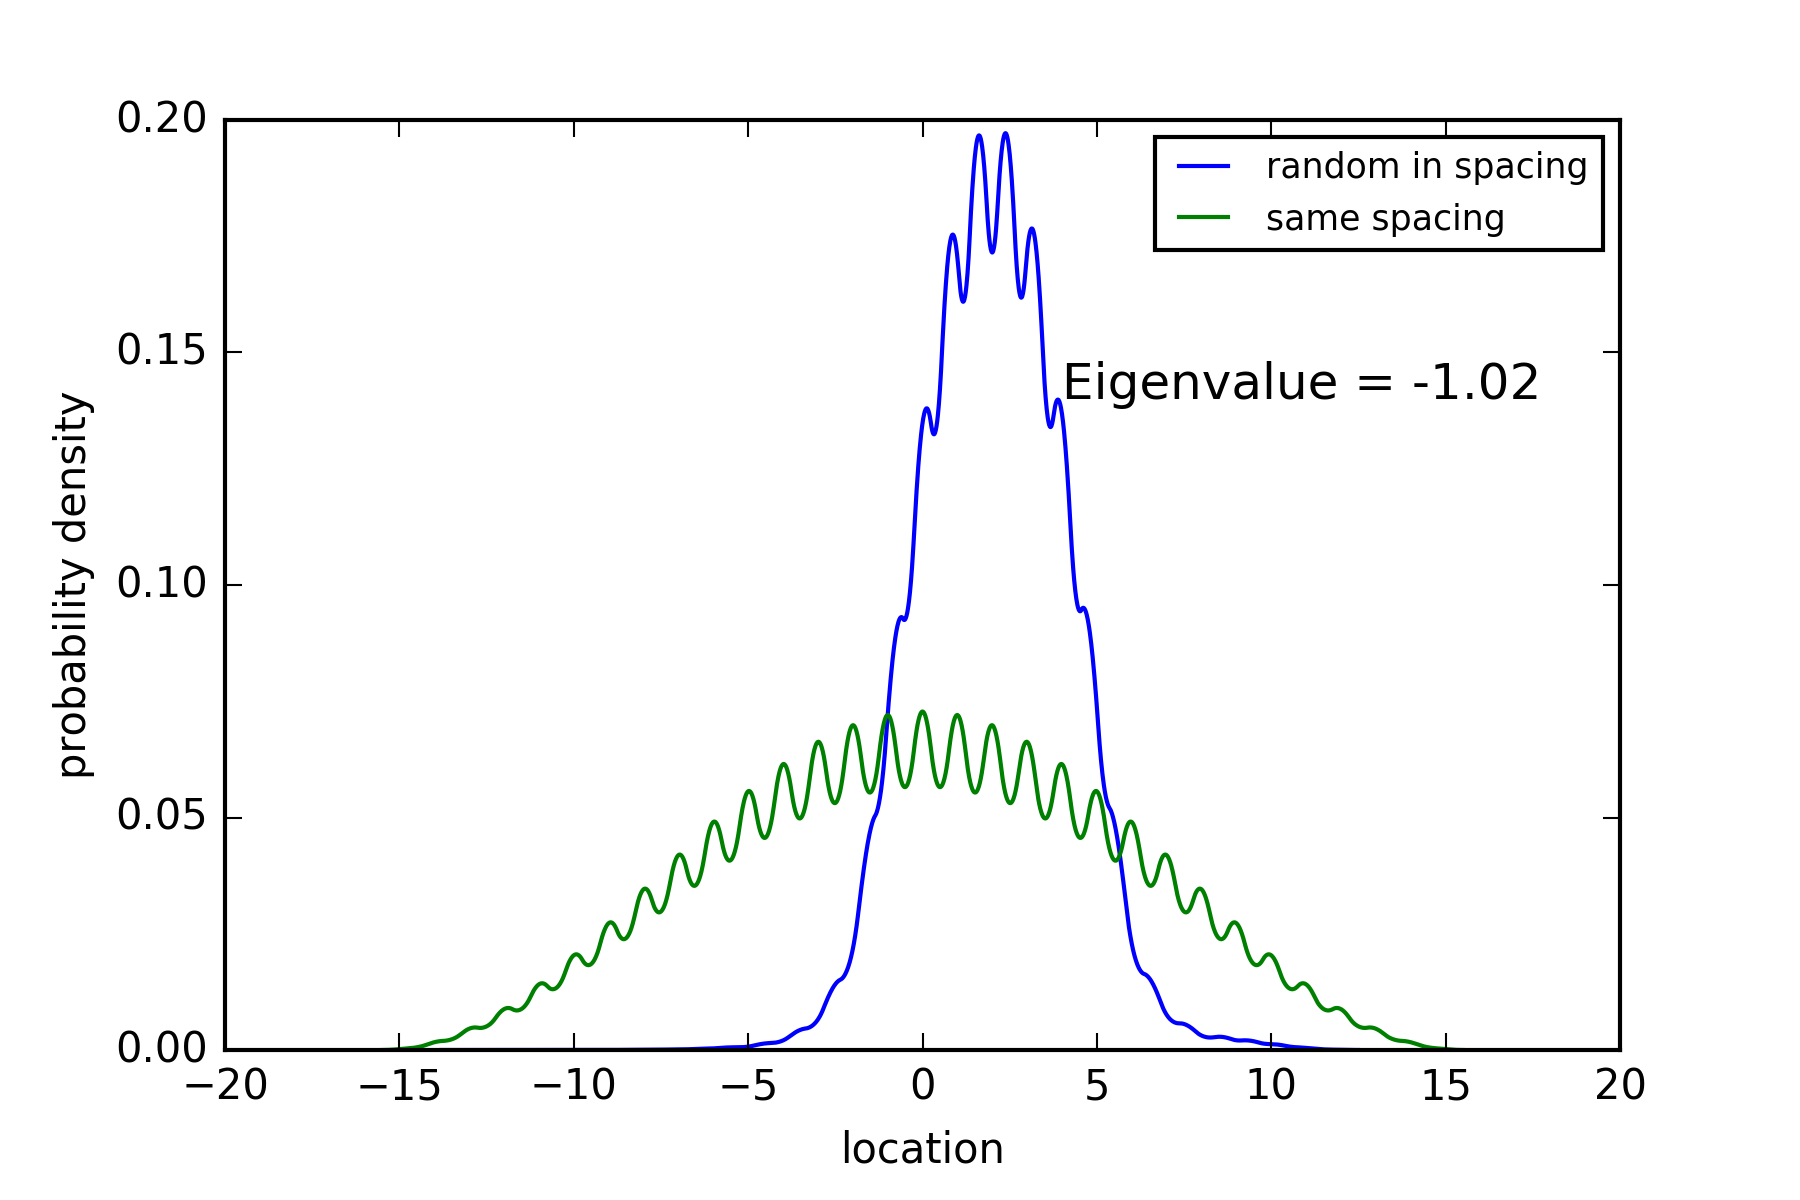
\includegraphics[width=1.1\linewidth]{Graphics/1_0_1th_Lowest_Rand0_8.png}
  \captionof{figure}{Lowest eigenvalue, $V_0l=1$, $\{p_1,p_2\}=\{0.8,1.0\}$}
  \label{fig:Area1_1thlowestRand0.8}
\end{minipage}\qquad
\begin{minipage}{.45\textwidth}
  \centering
  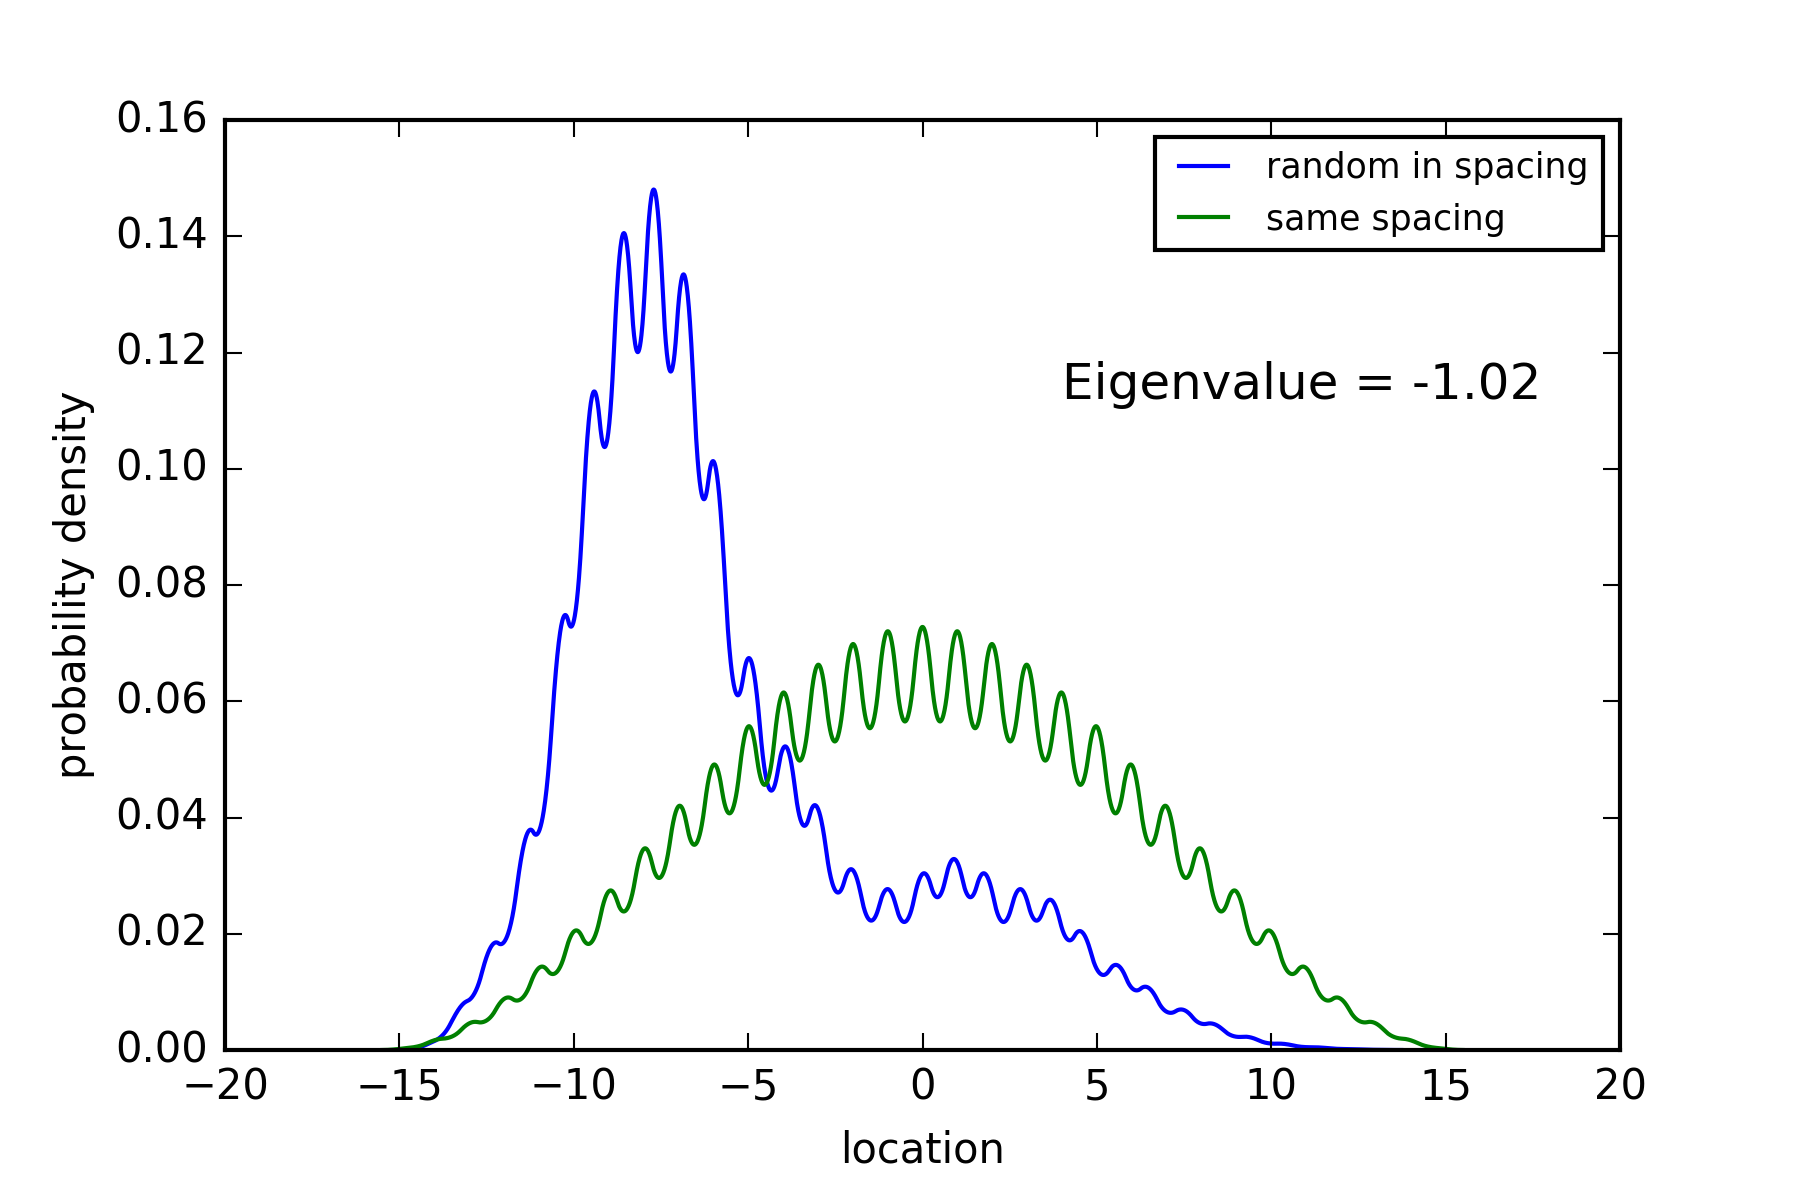
\includegraphics[width=1.1\linewidth]{Graphics/1_0_1th_Lowest_Rand0_9.png}
  \captionof{figure}{Lowest eigenvalue, $V_0l=1$, $\{p_1,p_2\}=\{0.9,1.0\}$}
  \label{fig:Area1_1thlowestRand0.9}
\end{minipage}
\end{figure}

\begin{figure}[!htbh]
\centering
\begin{minipage}{.45\textwidth}
  \centering
  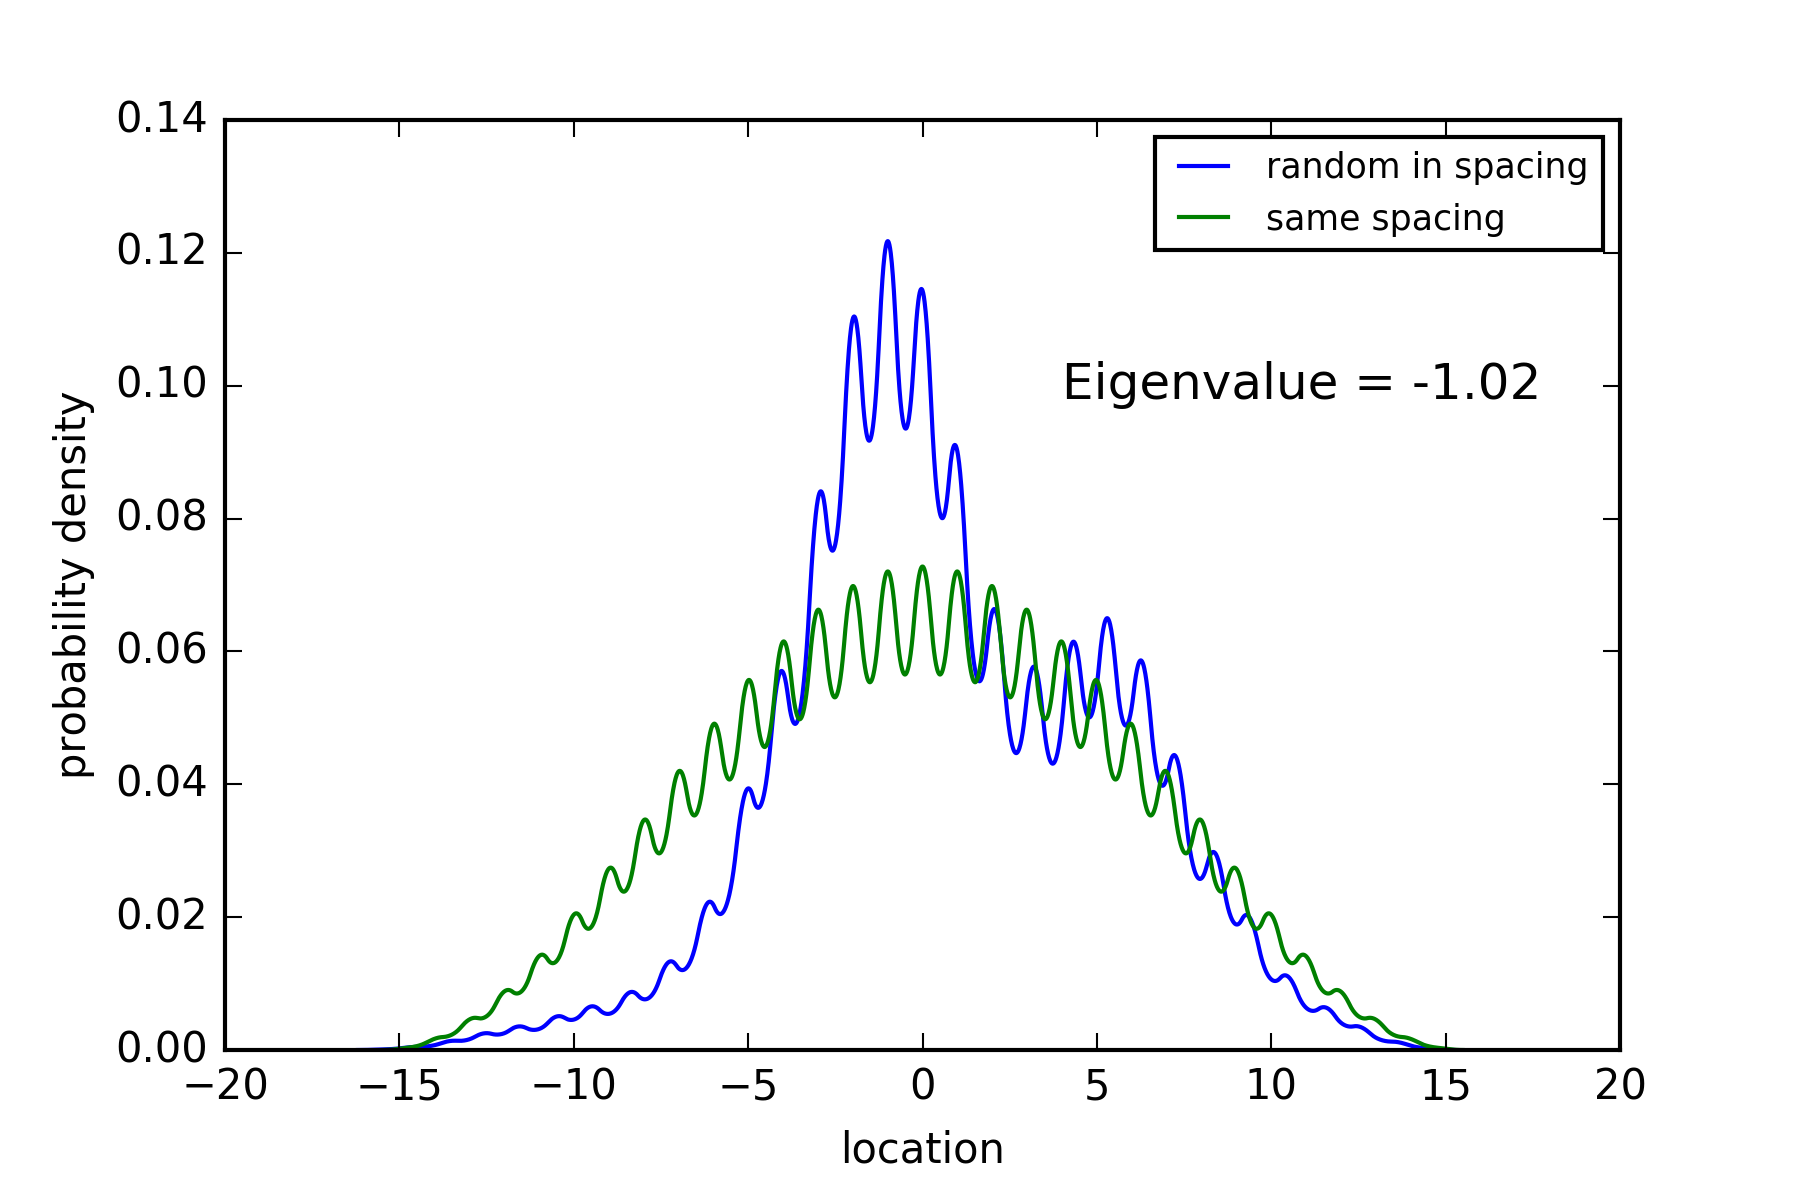
\includegraphics[width=1.1\linewidth]{Graphics/1_0_1th_Lowest_Rand1_1.png}
  \captionof{figure}{Lowest eigenvalue, $V_0l=1$, $\{p_1,p_2\}=\{1.1,1.0\}$}
  \label{fig:Area1_1thlowestRand1.1}
\end{minipage}\qquad
\begin{minipage}{.45\textwidth}
  \centering
  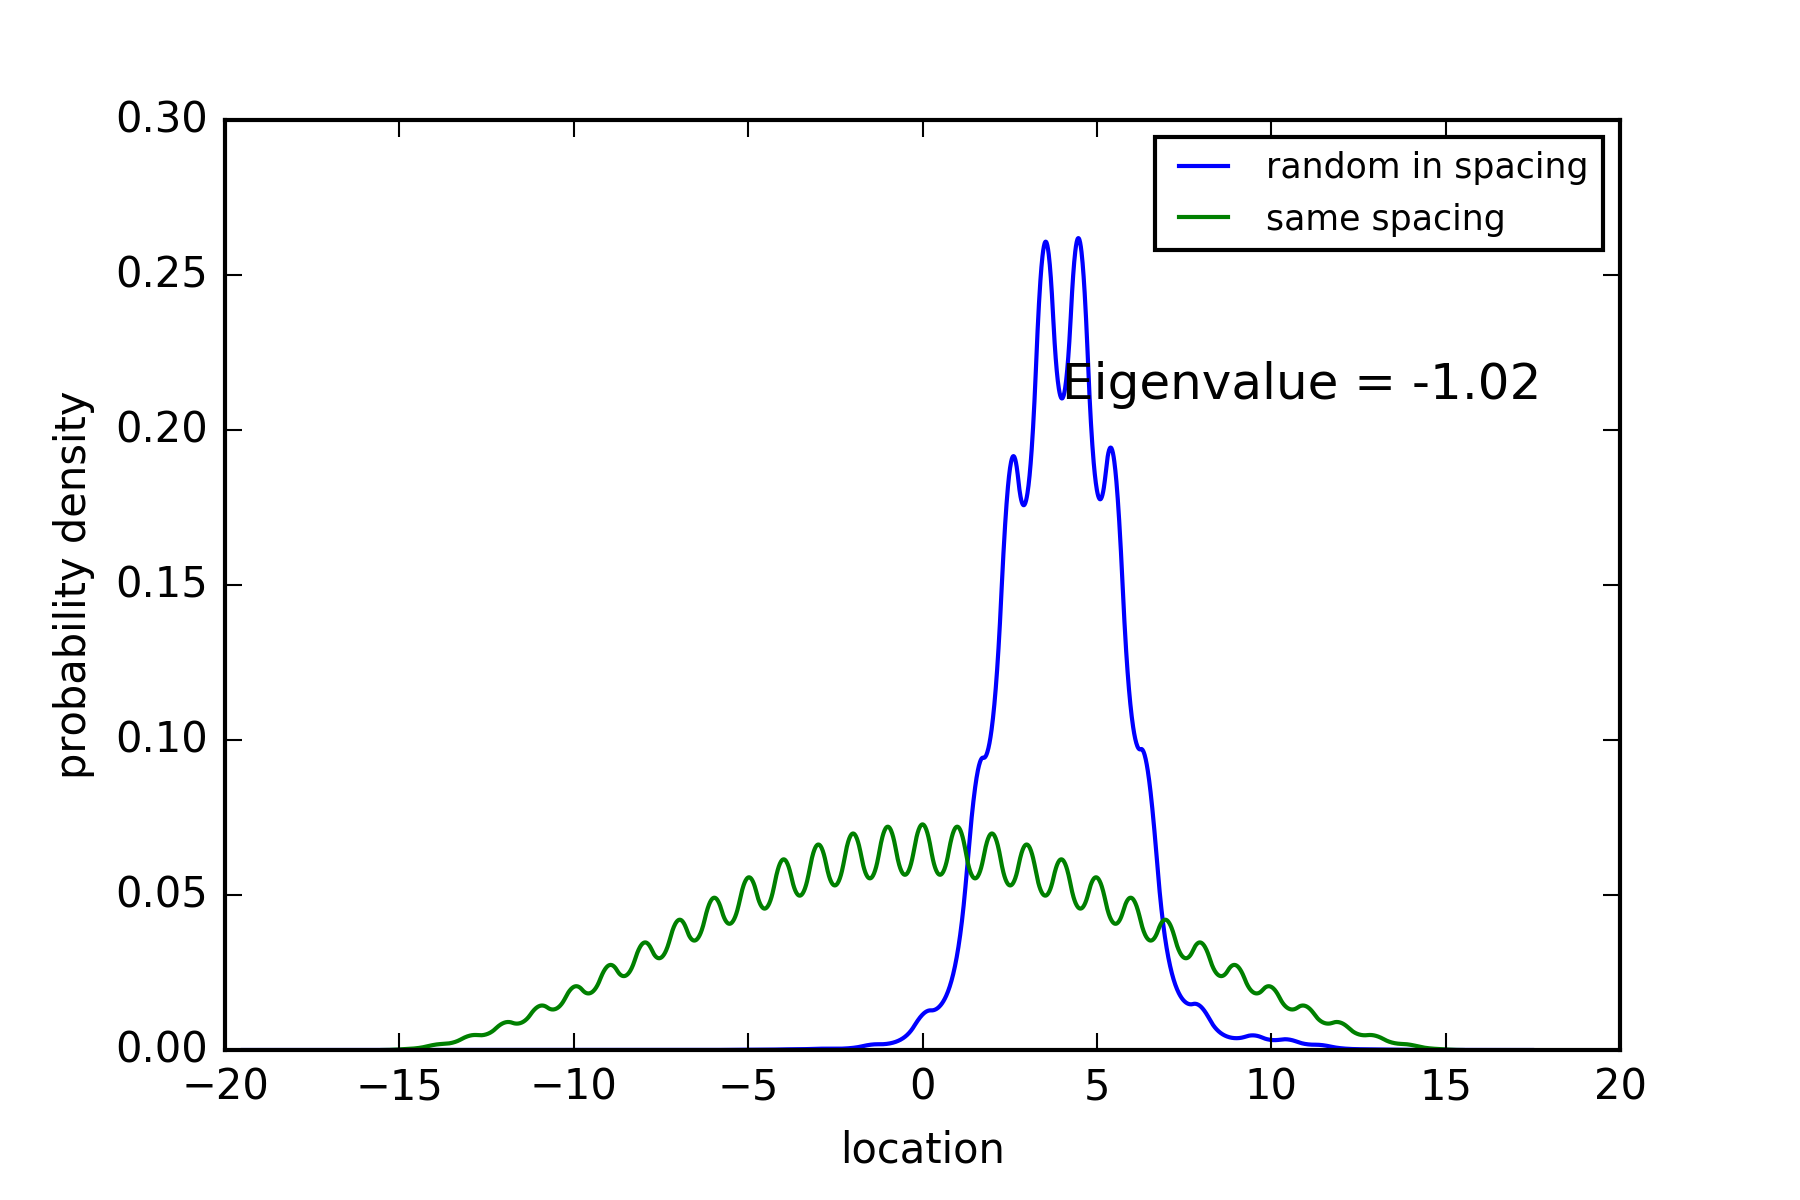
\includegraphics[width=1.1\linewidth]{Graphics/1_0_1th_Lowest_Rand1_5.png}
  \captionof{figure}{Lowest eigenvalue, $V_0l=1$, $\{p_1,p_2\}=\{1.5,1.0\}$}
  \label{fig:Area1_1thlowestRand1.5}
\end{minipage}
\end{figure}

\newpage
The following are figures for the eigenstate of the disordered system when $V_0l$ is equal to 10.

\begin{figure}[!htbh]
\centering
\begin{minipage}{.45\textwidth}
  \centering
  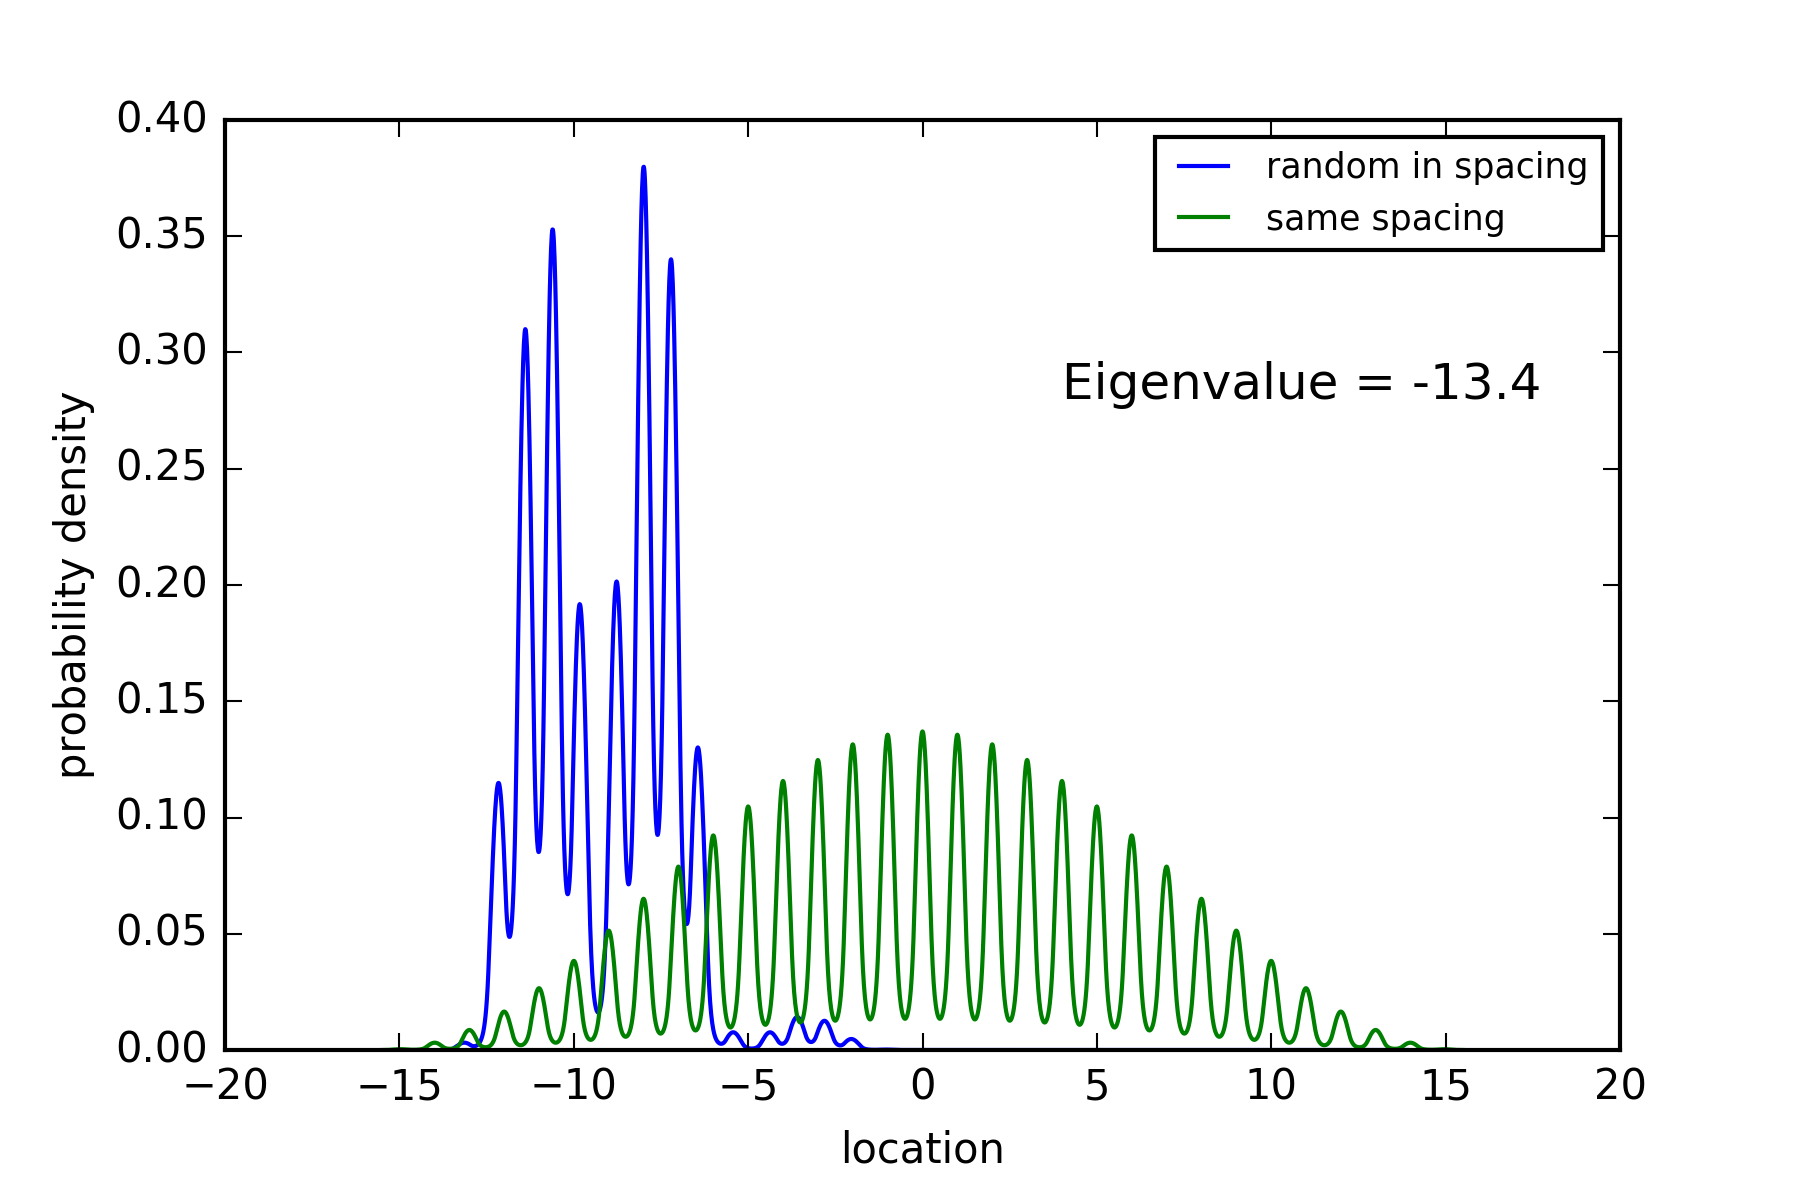
\includegraphics[width=1.1\linewidth]{Graphics/10_0_1th_Lowest_Rand0_8.png}
  \captionof{figure}{Lowest eigenvalue, $V_0l=10.0$ ,$\{p_1,p_2\}=\{0.8,1.0\}$}
  \label{fig:Area10_1thlowestRand0.8}
\end{minipage}\qquad
\begin{minipage}{.45\textwidth}
  \centering
  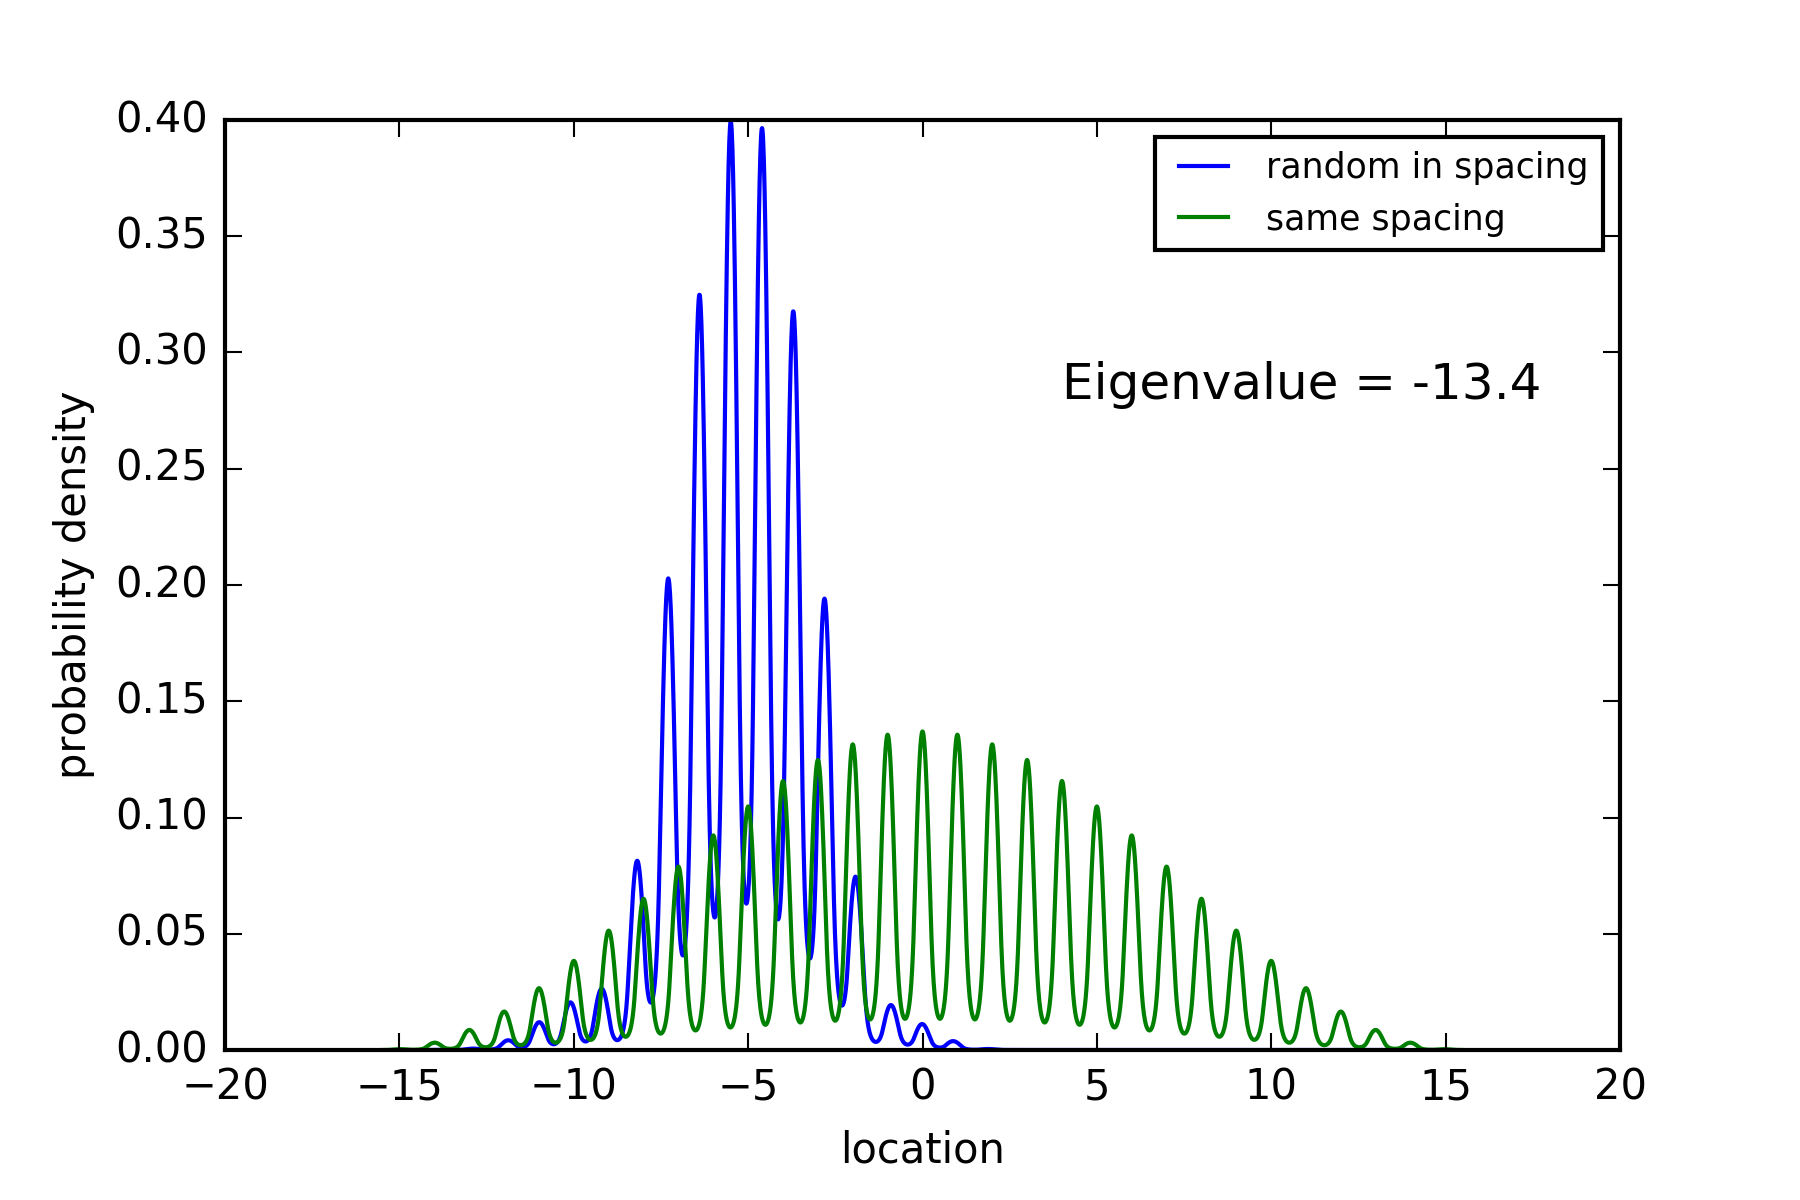
\includegraphics[width=1.1\linewidth]{Graphics/10_0_1th_Lowest_Rand0_9.png}
  \captionof{figure}{Lowest eigenvalue, $V_0l=10.0$, $\{p_1,p_2\}=\{0.9,1.0\}$}
  \label{fig:Area10_1thlowestRand0.9}
\end{minipage}
\end{figure}

\begin{figure}[!htbh]
\centering
\begin{minipage}{.45\textwidth}
  \centering
  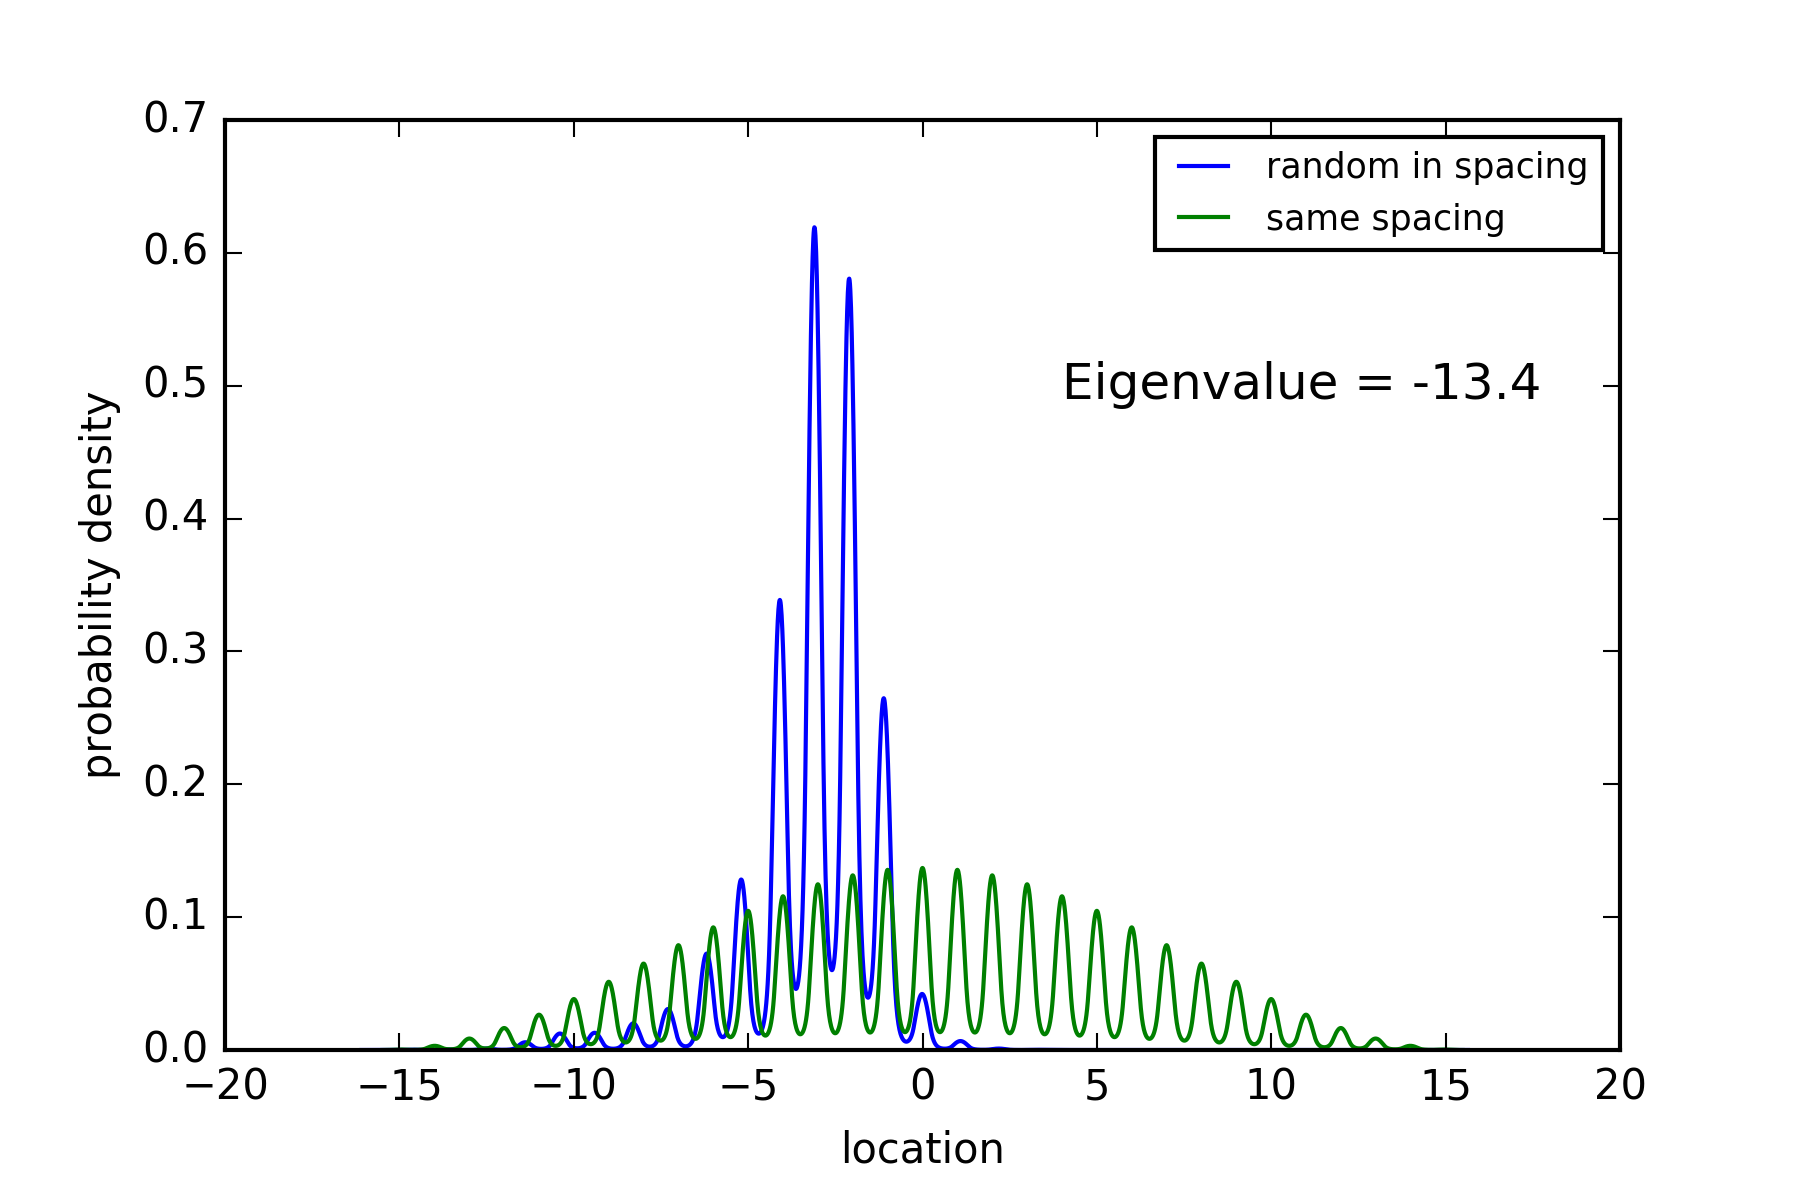
\includegraphics[width=1.1\linewidth]{Graphics/10_0_1th_Lowest_Rand1_1.png}
  \captionof{figure}{Lowest eigenvalue, $V_0l=10.0$, $\{p_1,p_2\}=\{1.1,1.0\}$}
  \label{fig:Area10_1thlowestRand1.1}
\end{minipage}\qquad
\begin{minipage}{.45\textwidth}
  \centering
  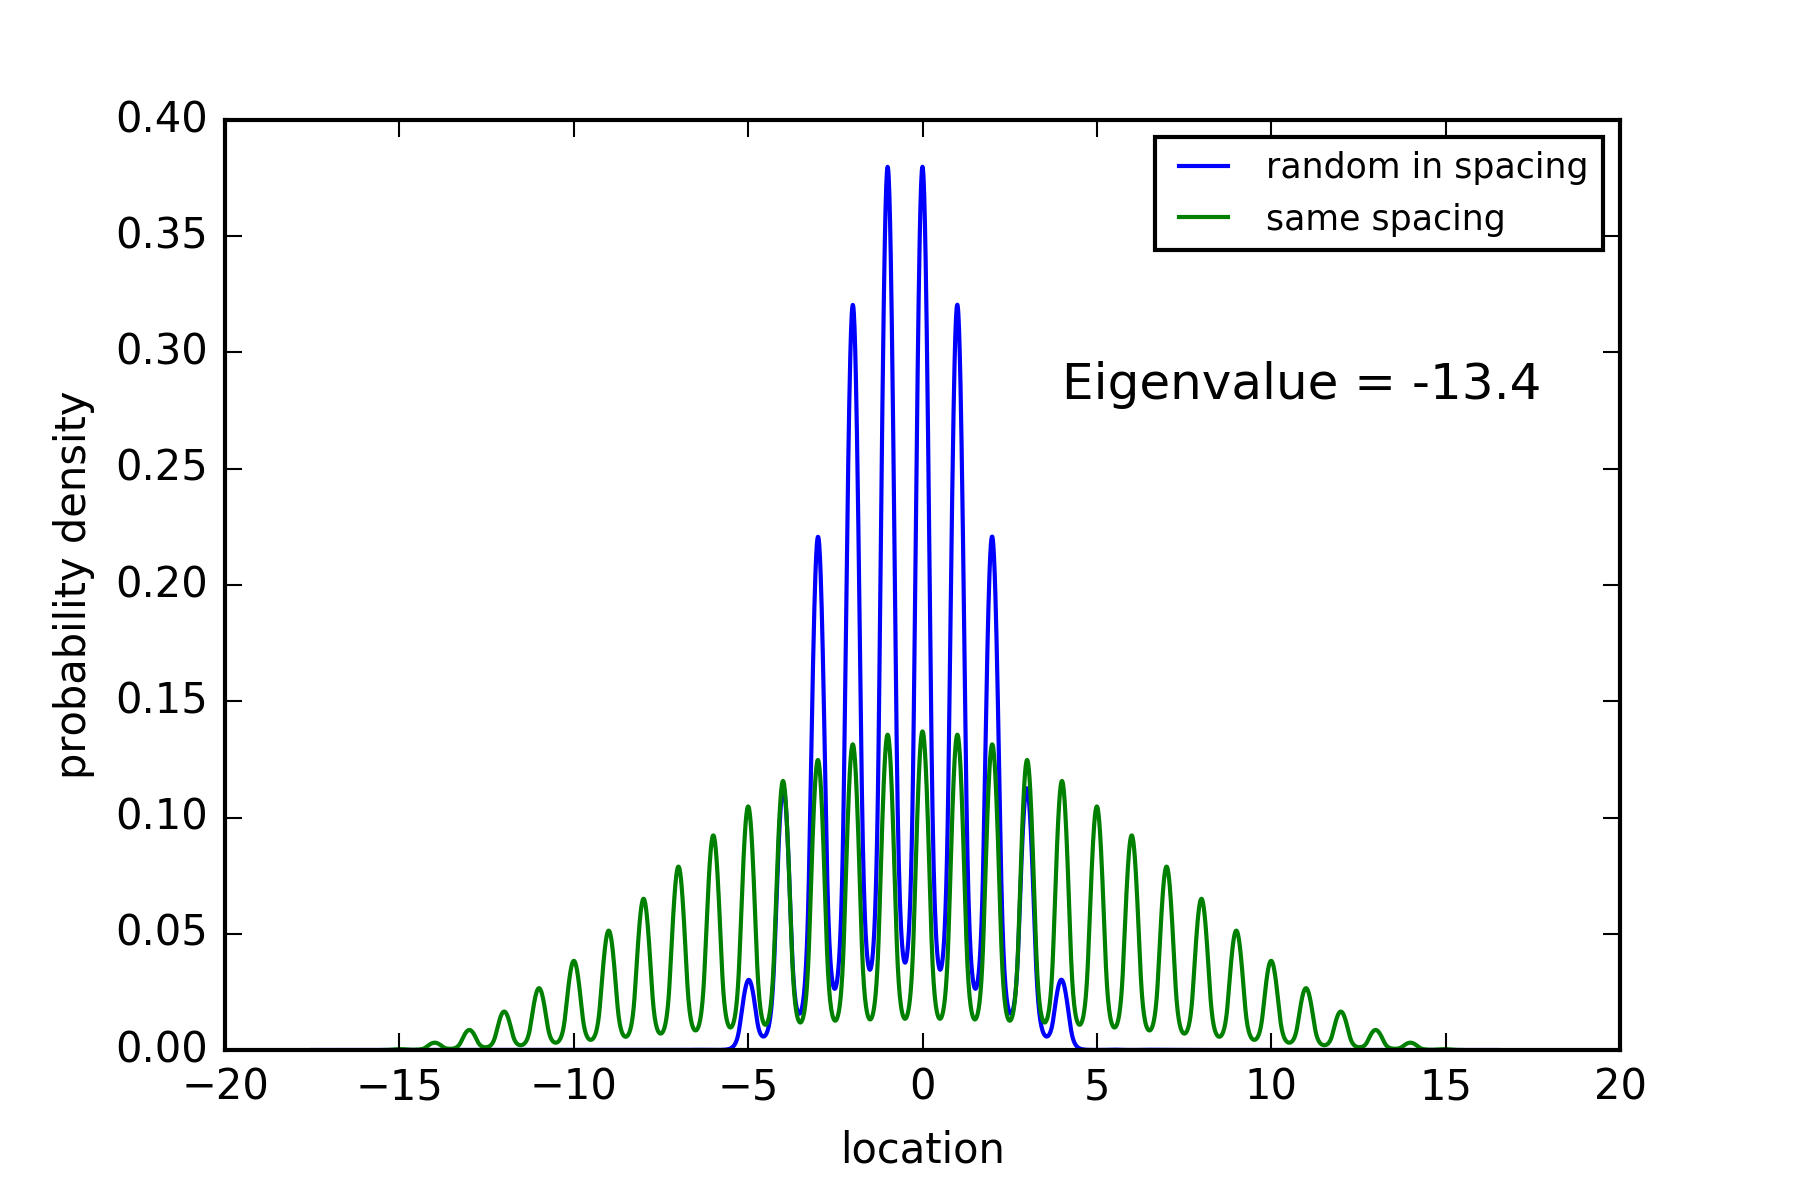
\includegraphics[width=1.1\linewidth]{Graphics/10_0_1th_Lowest_Rand1_5.png}
  \captionof{figure}{Lowest eigenvalue, $V_0l=10.0$, $\{p_1,p_2\}=\{1.5,1.0\}$}
  \label{fig:Area10_1thlowestRand1.5}
\end{minipage}
\end{figure}

% modified Wed 15:15 pm

The following are figures for the eigenstate corresponding to the second lowest eigenenergy. Again, $V_0l$ is equal to 1 for the first 4 figures, and 10 for the other 4 figures. They are in the same order as the eigenstates for the lowest eigenenergy.

%2nd lowest, Vl = 1.0
\begin{figure}[!htbh]
\centering
\begin{minipage}{.45\textwidth}
  \centering
  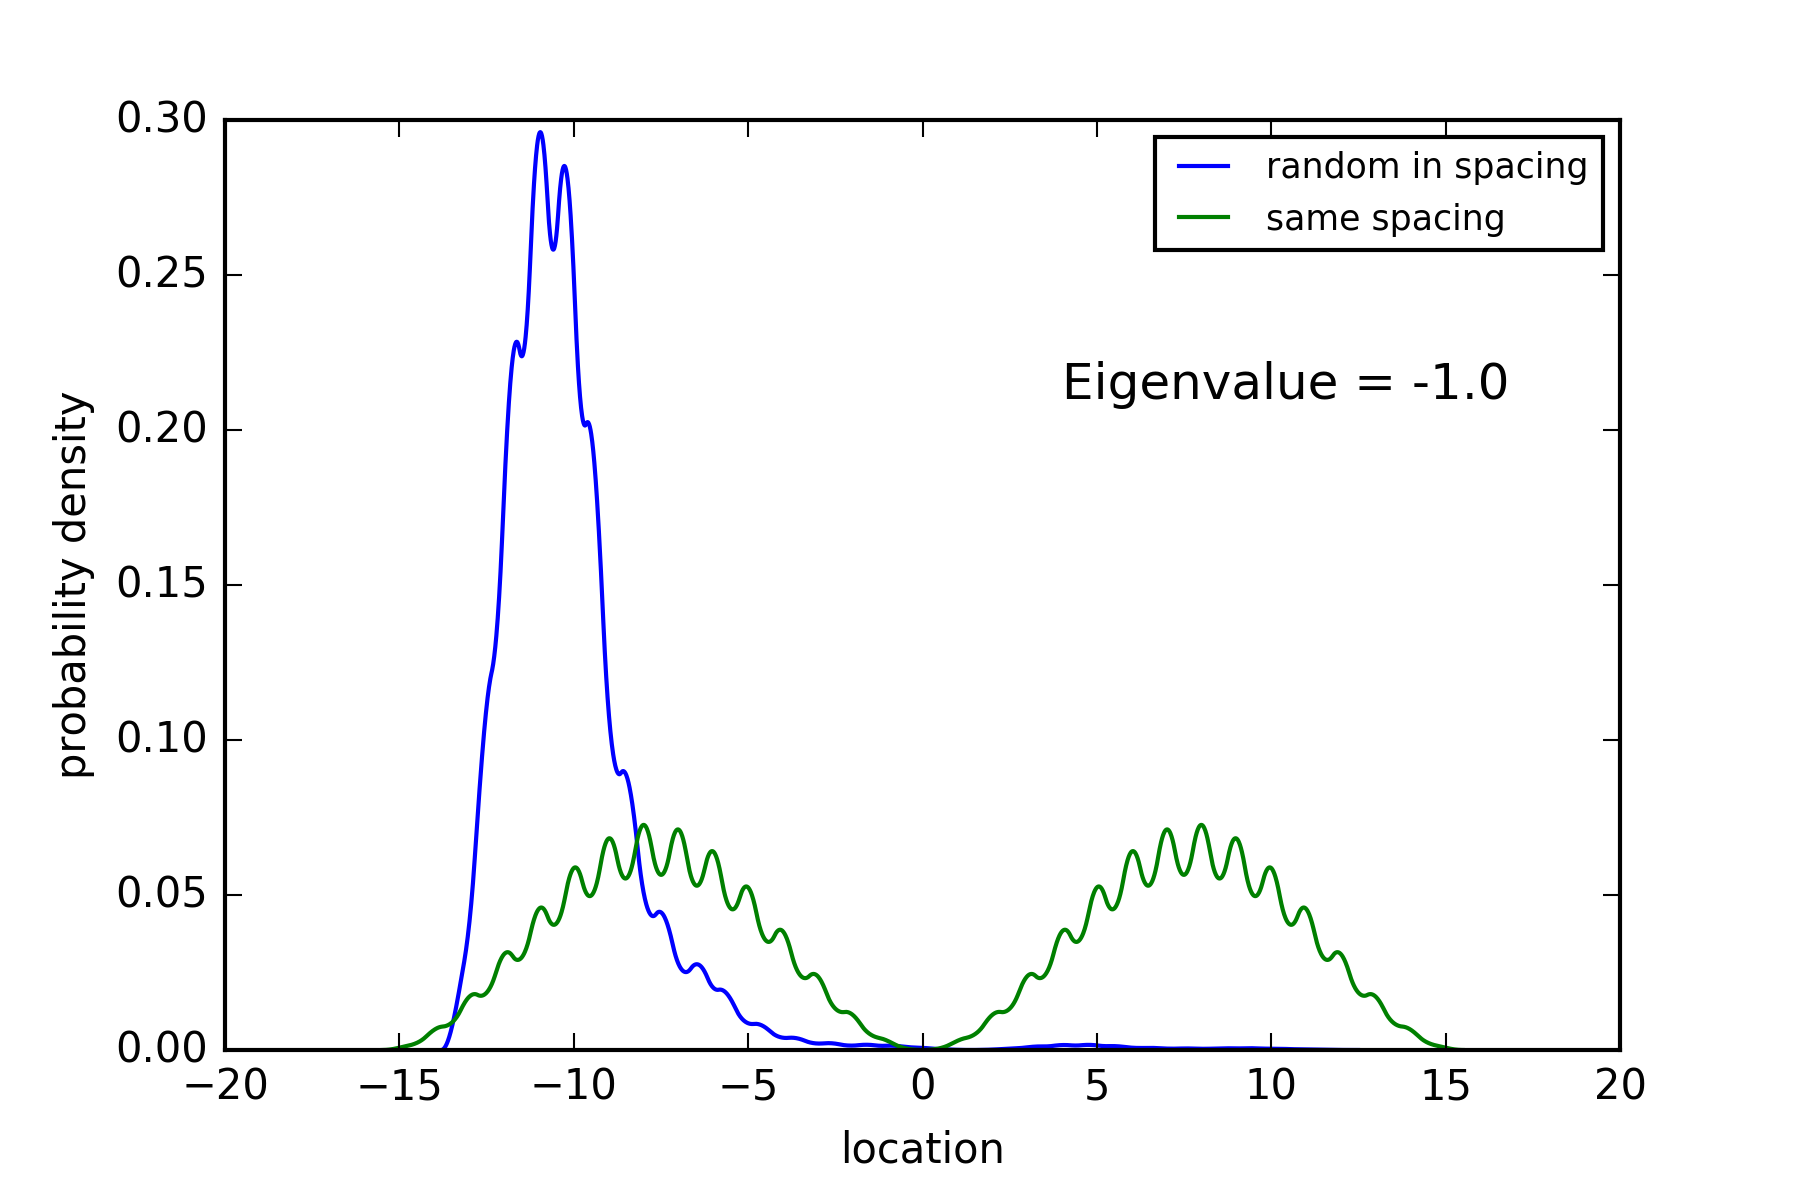
\includegraphics[width=1.1\linewidth]{Graphics/1_0_2th_Lowest_Rand0_8.png}
  \captionof{figure}{2nd Lowest eigenvalue, $V_0l=1.0$, $\{p_1,p_2\}=\{0.8,1.0\}$}
  \label{fig:Area1_2thlowestRand0.8}
\end{minipage}\qquad
\begin{minipage}{.45\textwidth}
  \centering
  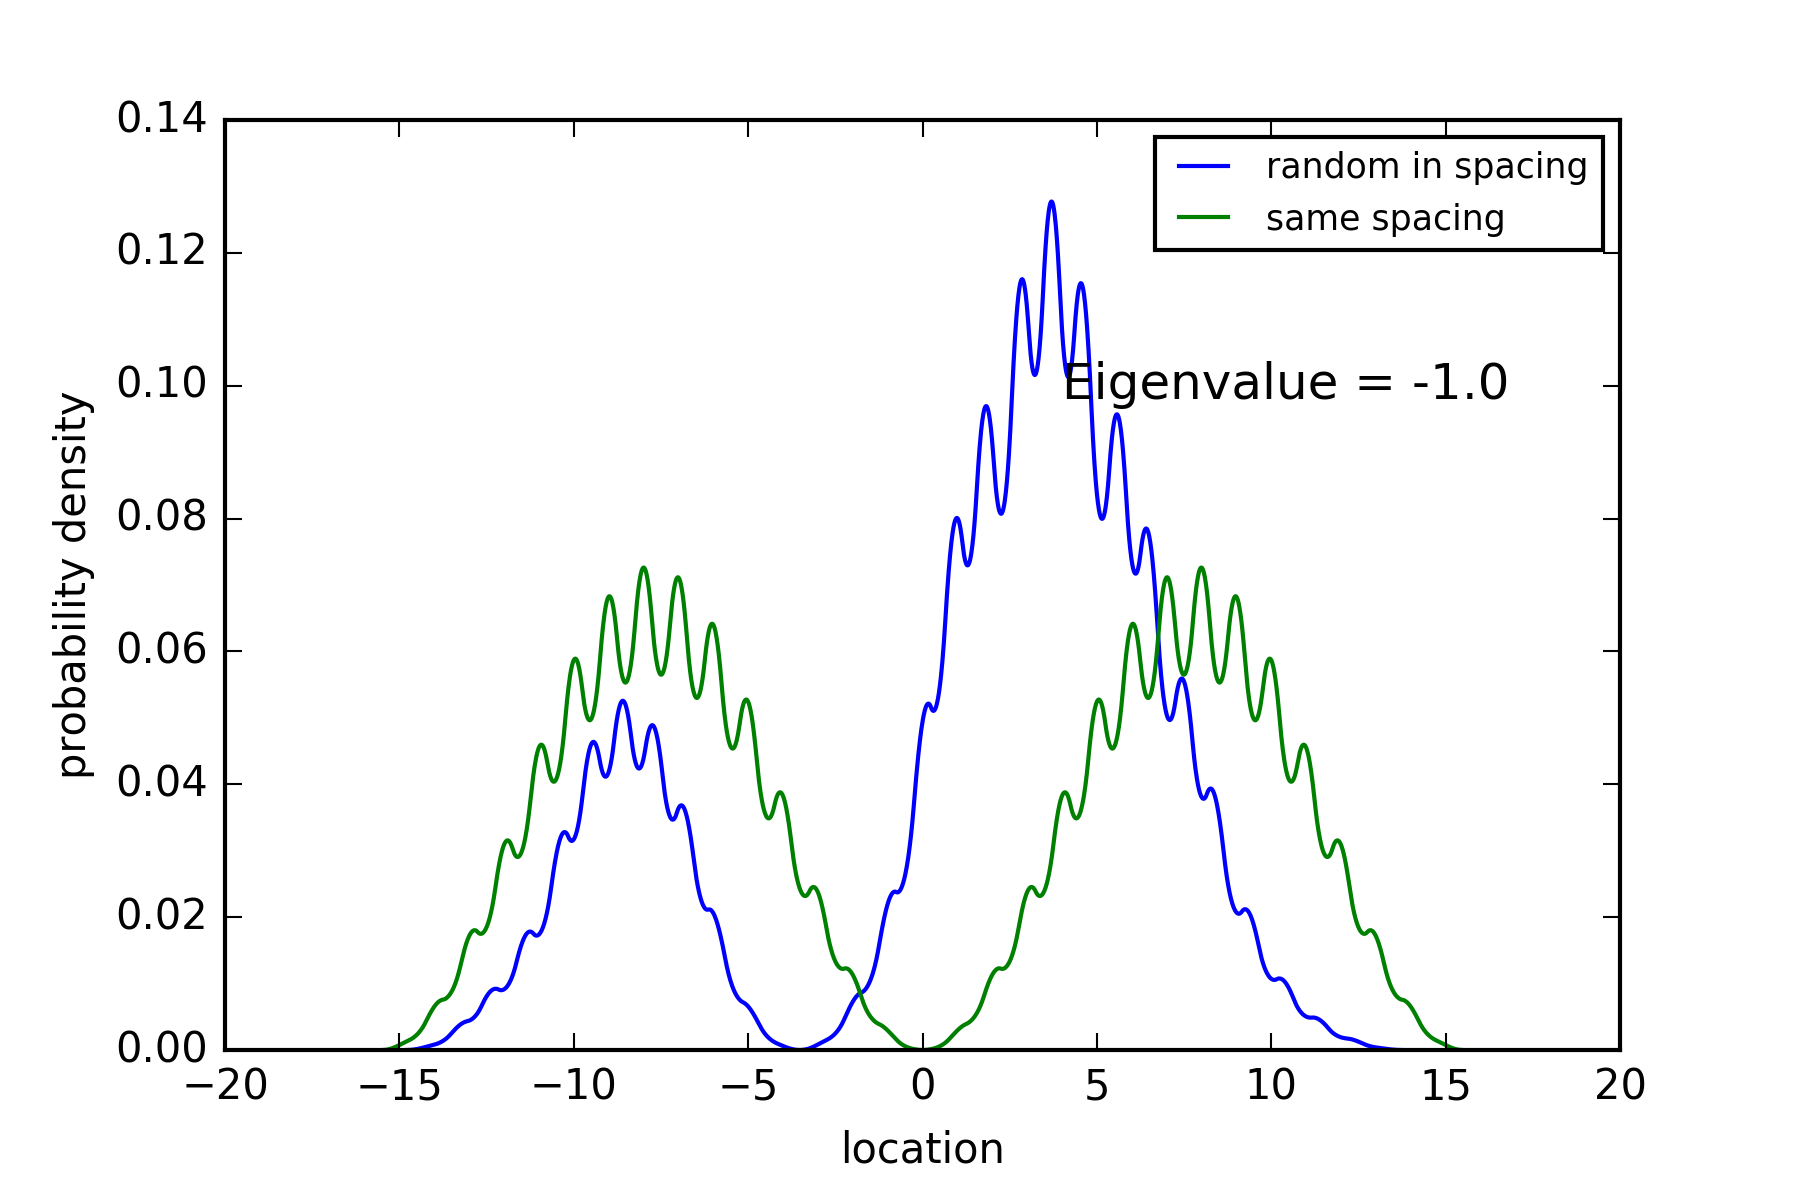
\includegraphics[width=1.1\linewidth]{Graphics/1_0_2th_Lowest_Rand0_9.png}
  \captionof{figure}{2nd Lowest eigenvalue, $V_0l=1.0$, $\{p_1,p_2\}=\{0.9,1.0\}$}
  \label{fig:Area1_2thlowestRand0.9}
\end{minipage}
\end{figure}

\begin{figure}[!htbh]
\centering
\begin{minipage}{.45\textwidth}
  \centering
  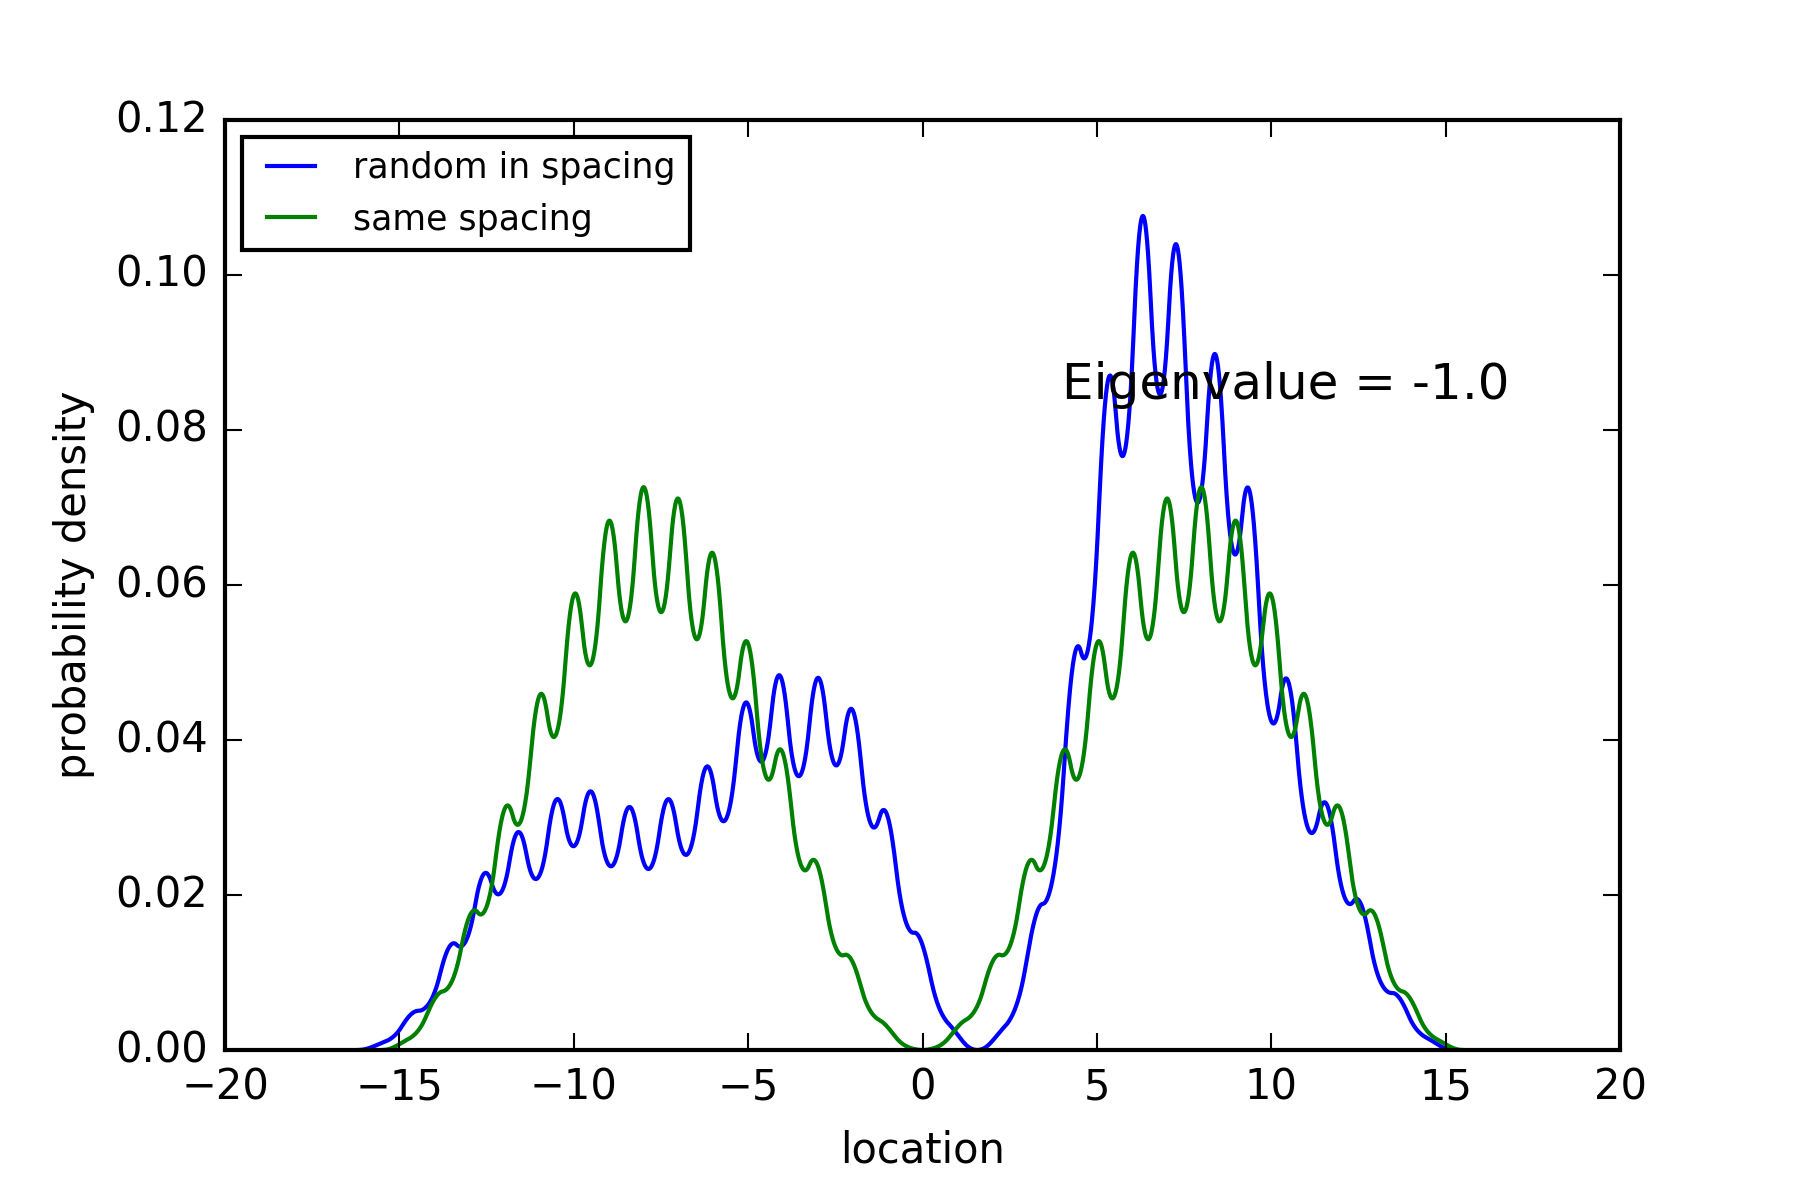
\includegraphics[width=1.1\linewidth]{Graphics/1_0_2th_Lowest_Rand1_1.png}
  \captionof{figure}{2nd Lowest eigenvalue, $V_0l = 1.0$, $\{p_1,p_2\}=\{1.1,1.0\}$}
  \label{fig:Area1_2thlowestRand1.1}
\end{minipage}\qquad
\begin{minipage}{.45\textwidth}
  \centering
  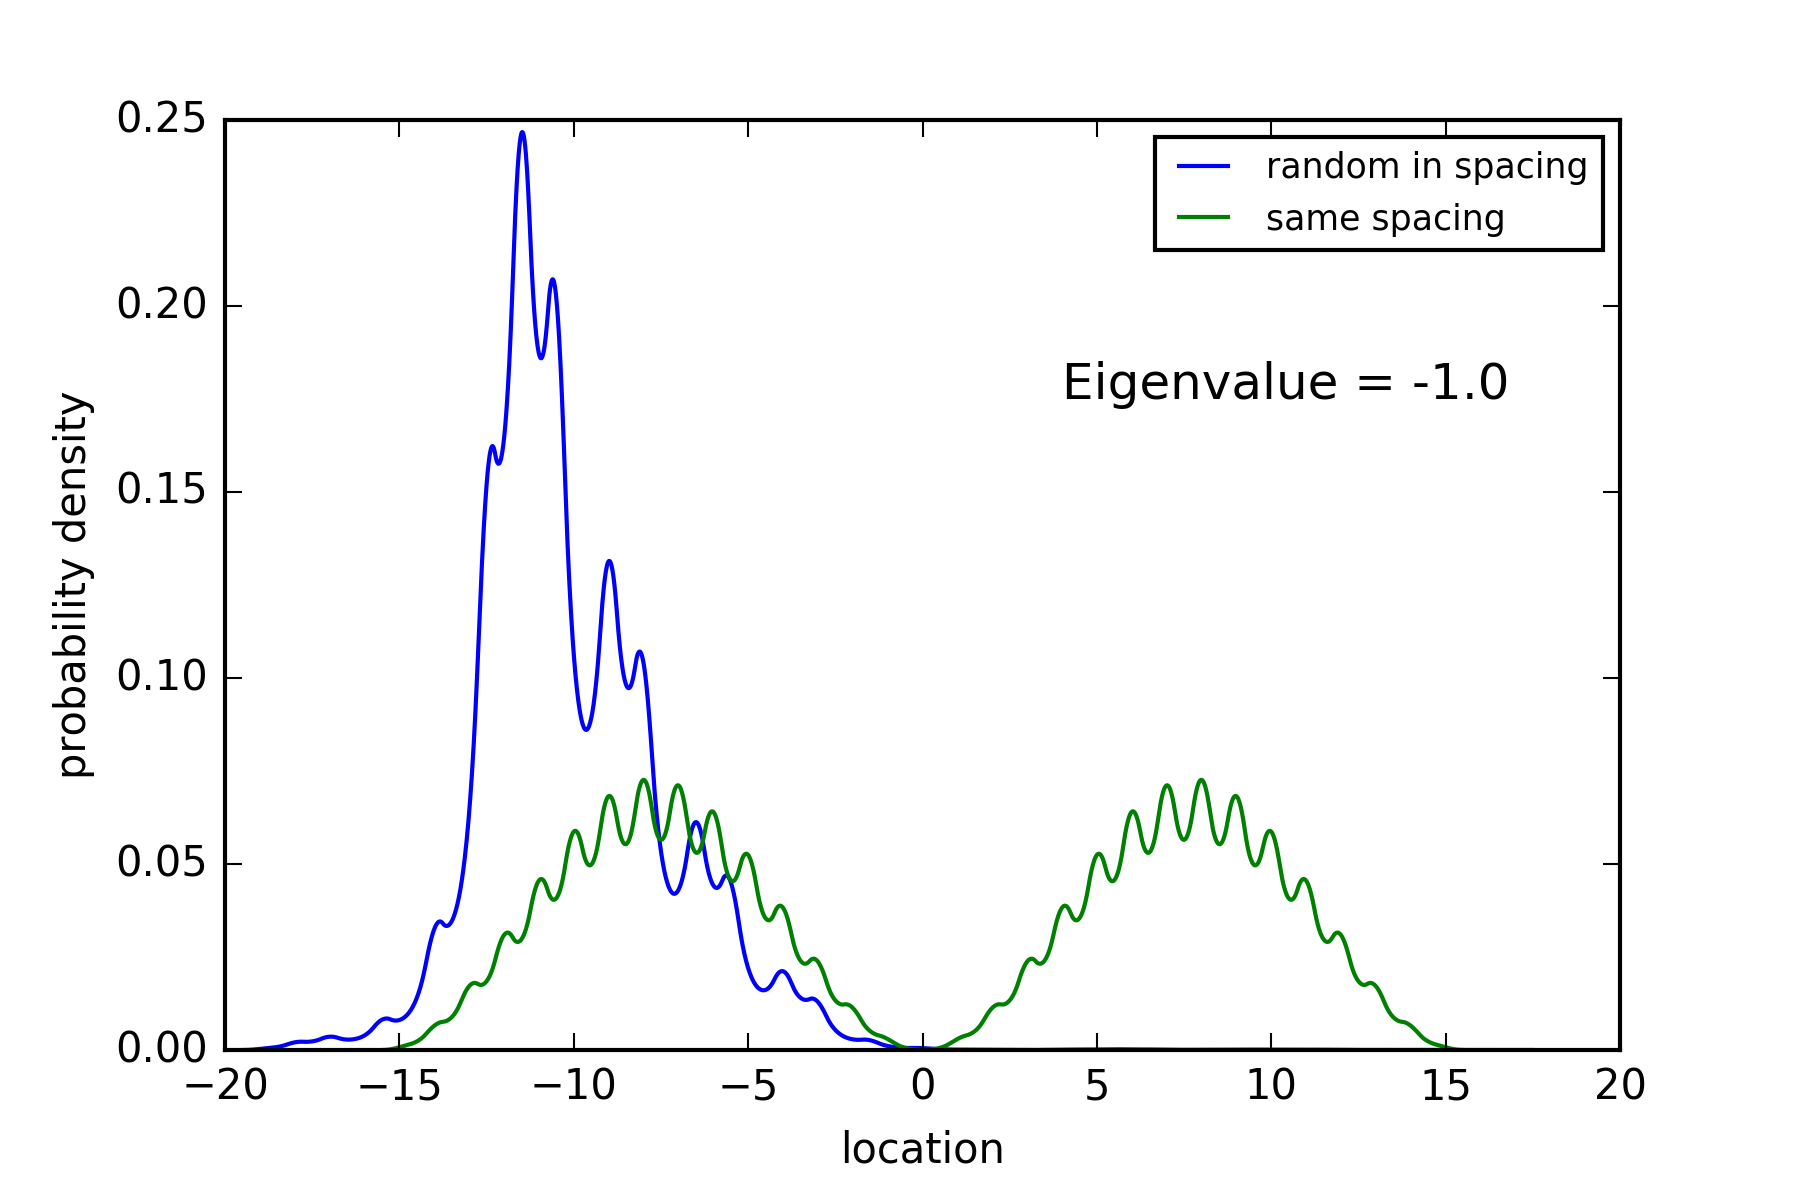
\includegraphics[width=1.1\linewidth]{Graphics/1_0_2th_Lowest_Rand1_5.png}
  \captionof{figure}{2nd Lowest eigenvalue, $V_0l=1.0$, $\{p_1,p_2\}=\{1.5,1.0\}$}
  \label{fig:Area1_2thlowestRand1.5}
\end{minipage}
\end{figure}

%2nd lowest, Vl = 10
\begin{figure}[!htbh]
\centering
\begin{minipage}{.45\textwidth}
  \centering
  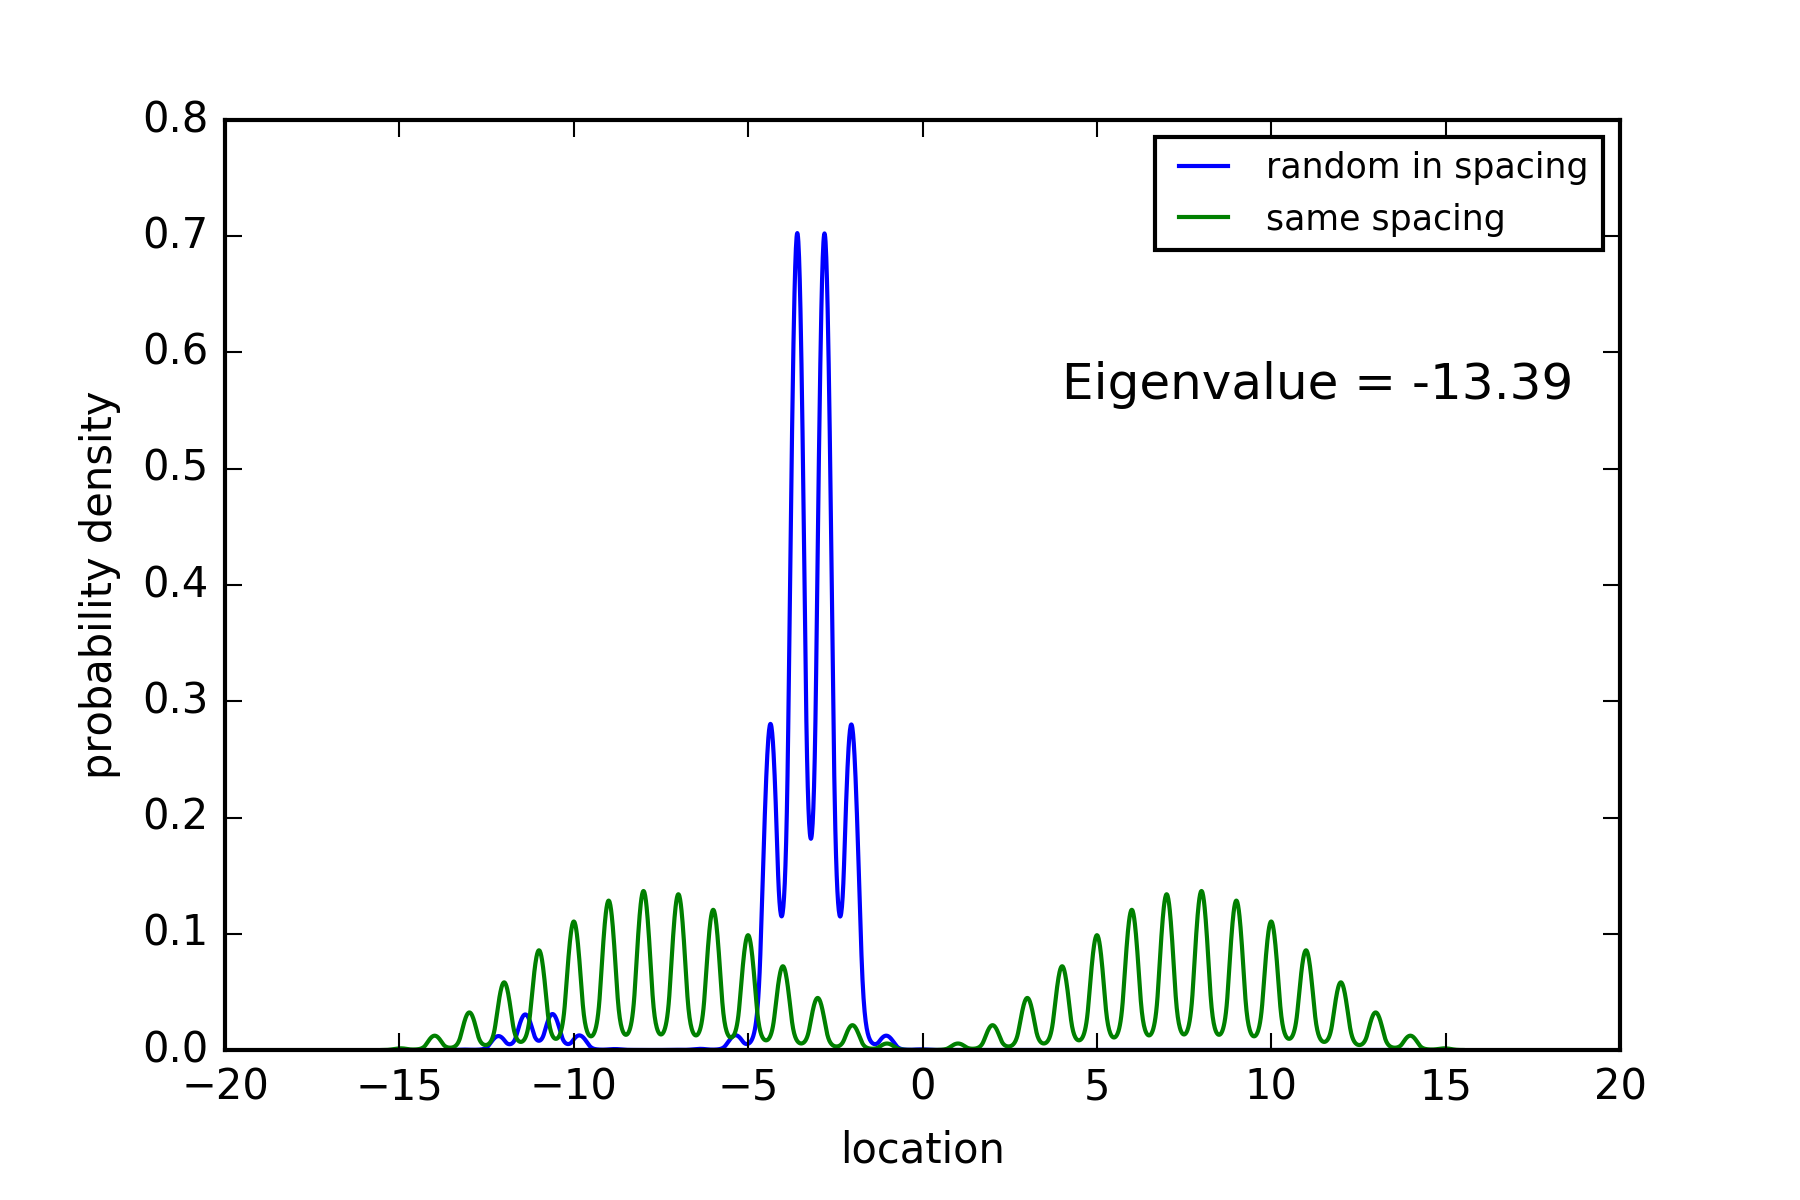
\includegraphics[width=1.1\linewidth]{Graphics/10_0_2th_Lowest_Rand0_8.png}
  \captionof{figure}{2nd Lowest eigenvalue, $V_0l=10.0$, $\{p_1,p_2\}=\{0.8,1.0\}$}
  \label{fig:Area10_2thlowestRand0.8}
\end{minipage}\qquad
\begin{minipage}{.45\textwidth}
  \centering
  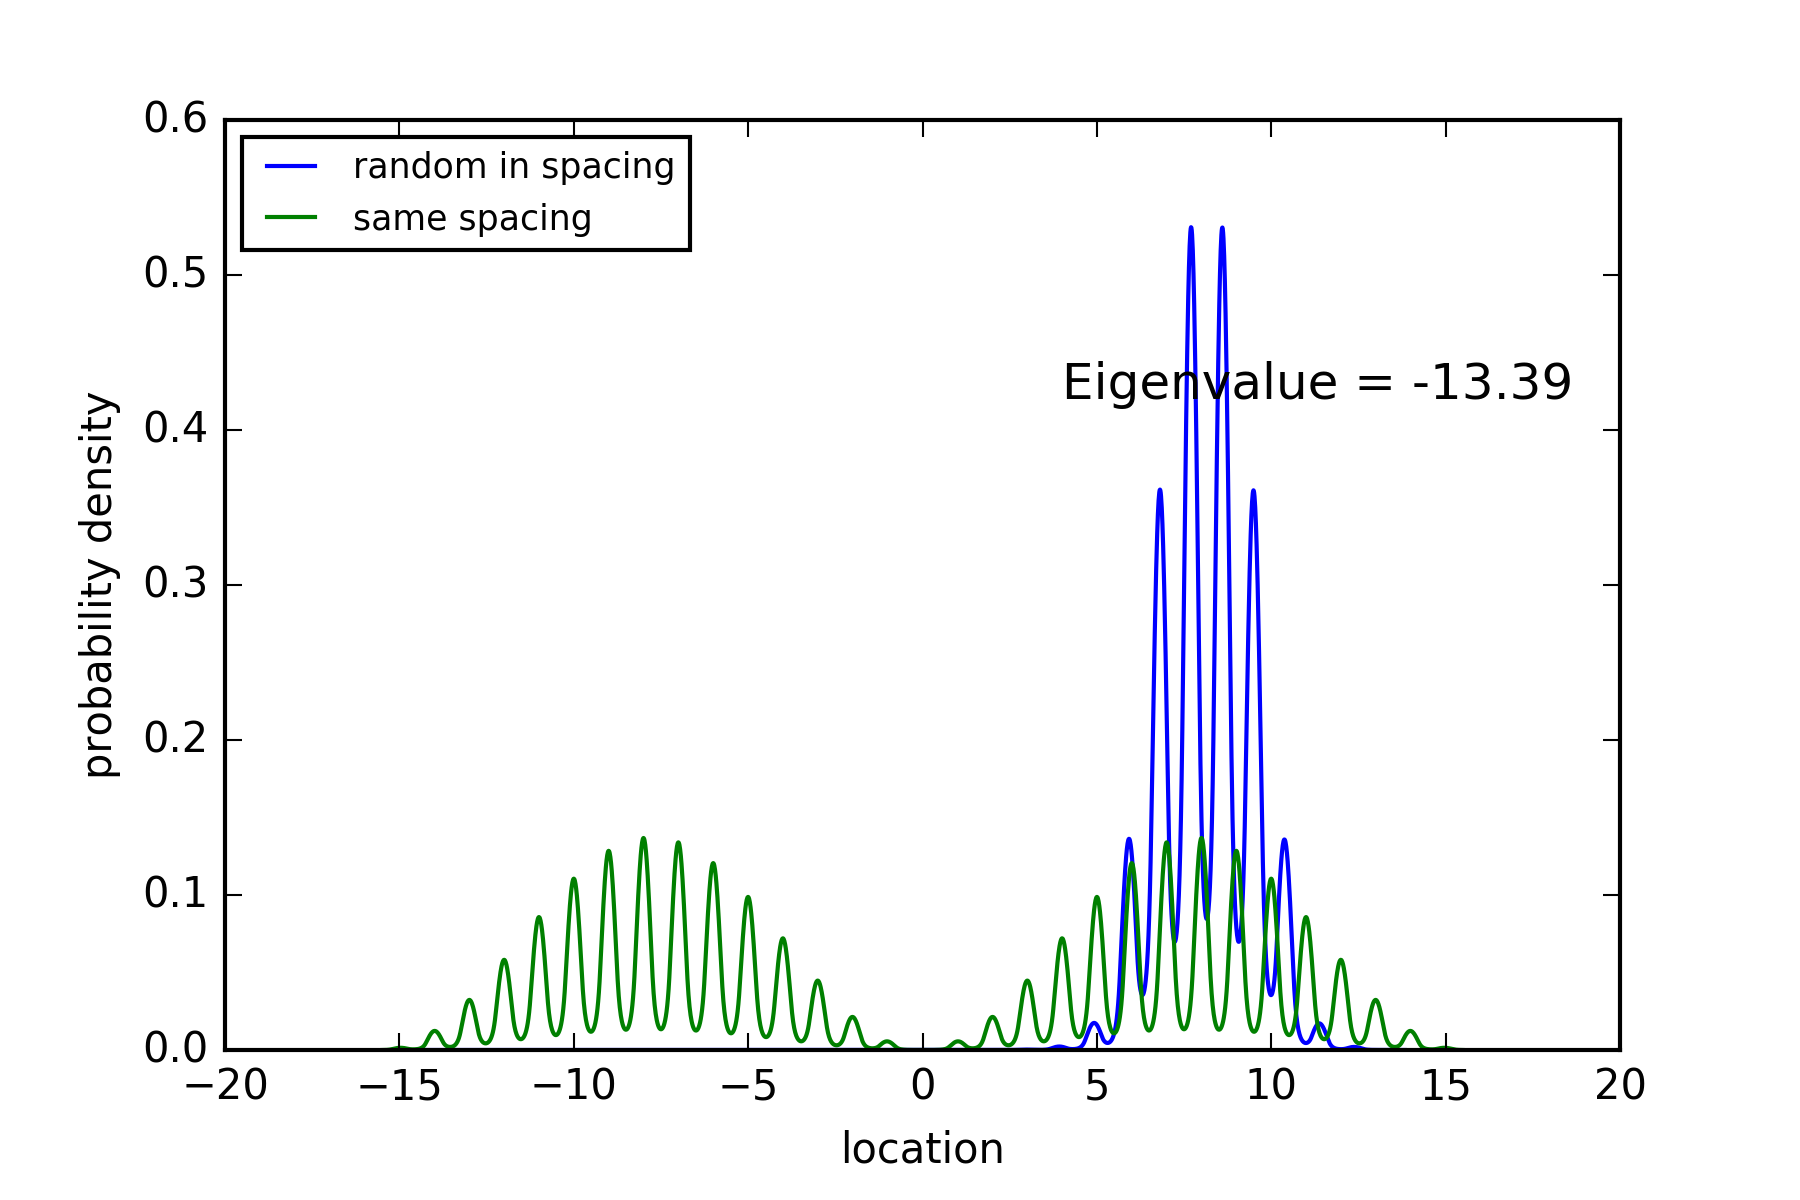
\includegraphics[width=1.1\linewidth]{Graphics/10_0_2th_Lowest_Rand0_9.png}
  \captionof{figure}{2nd Lowest eigenvalue, $V_0l=10.0$,$\{p_1,p_2\}=\{0.9,1.0\}$}
  \label{fig:Area10_2thlowestRand0.9}
\end{minipage}
\end{figure}

\begin{figure}[!htbh]
\centering
\begin{minipage}{.45\textwidth}
  \centering
  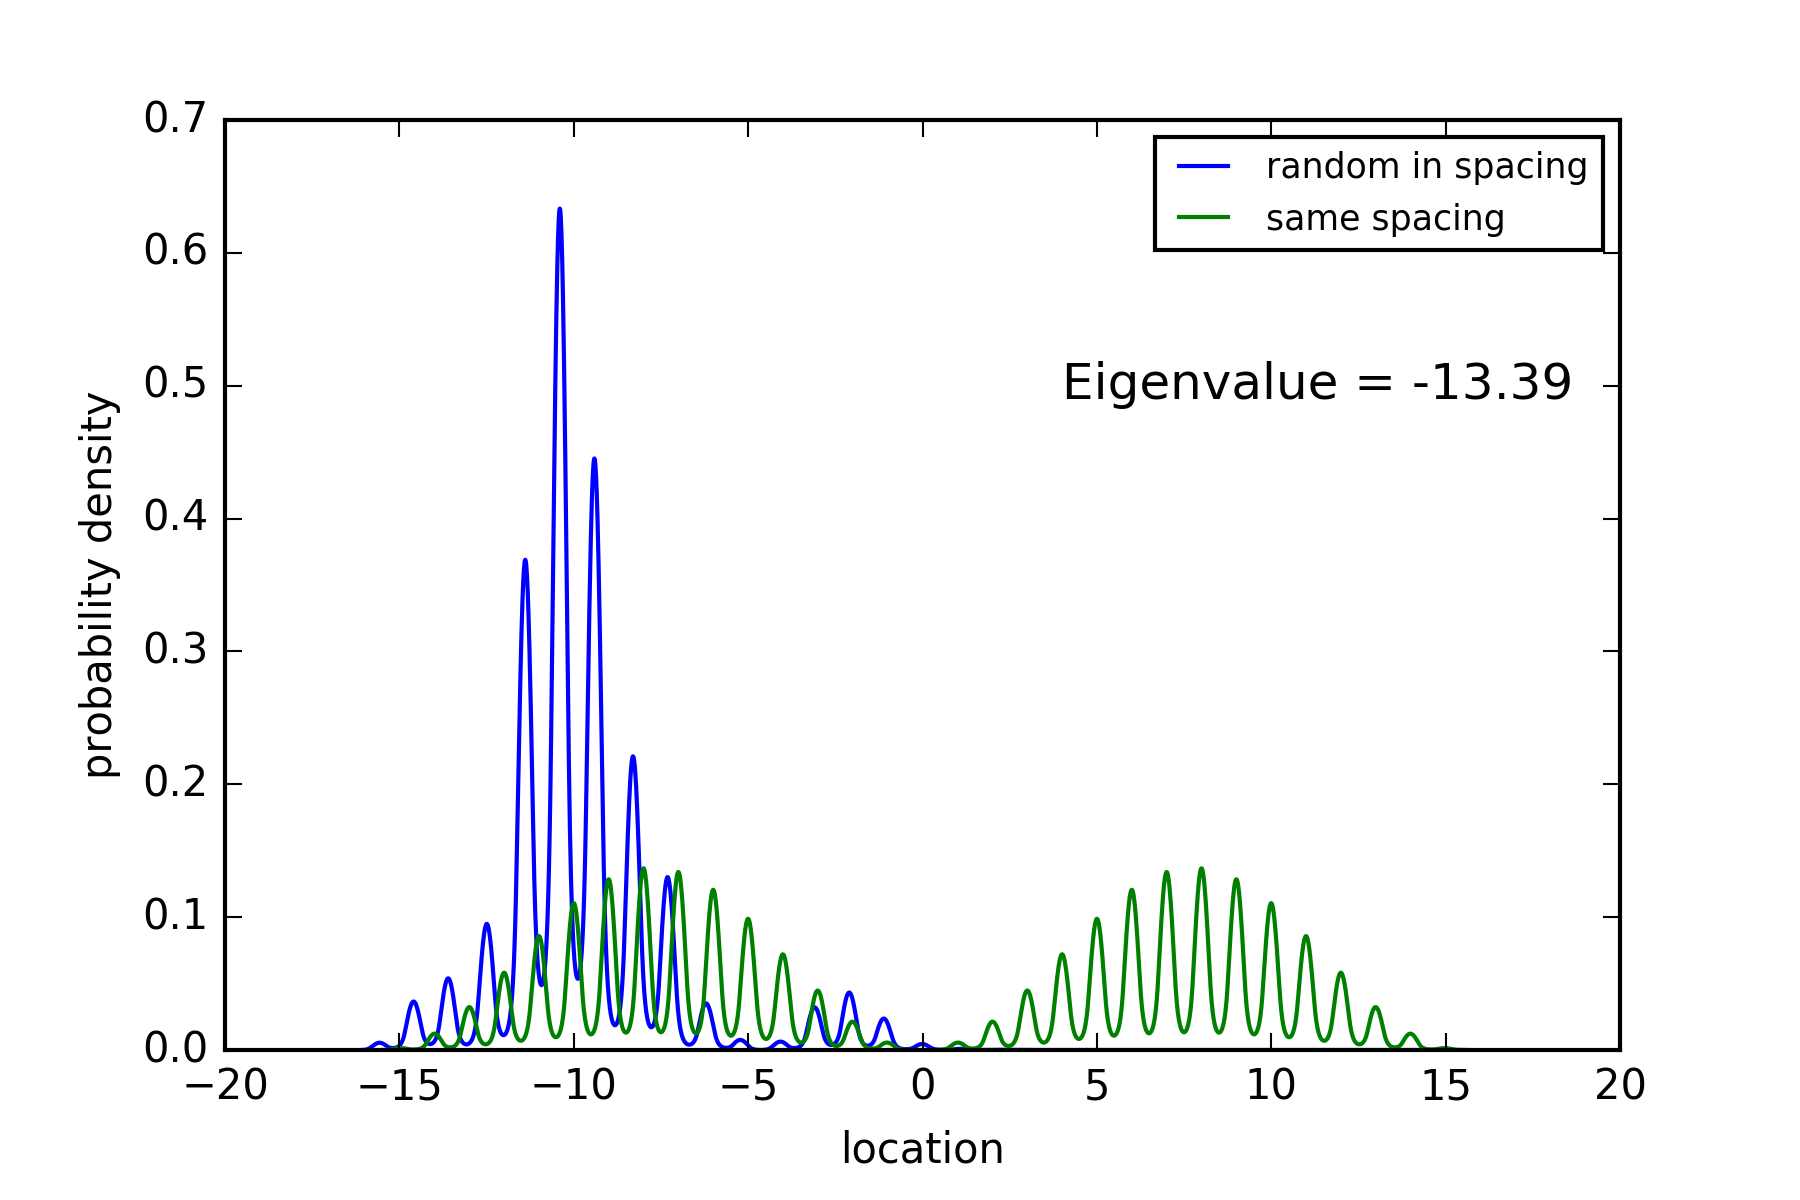
\includegraphics[width=1.1\linewidth]{Graphics/10_0_2th_Lowest_Rand1_1.png}
  \captionof{figure}{2nd Lowest eigenvalue, $V_0l=10.0$, $\{p_1,p_2\}=\{1.1,1.0\}$}
  \label{fig:Area10_2thlowestRand1.1}
\end{minipage}\qquad
\begin{minipage}{.45\textwidth}
  \centering
  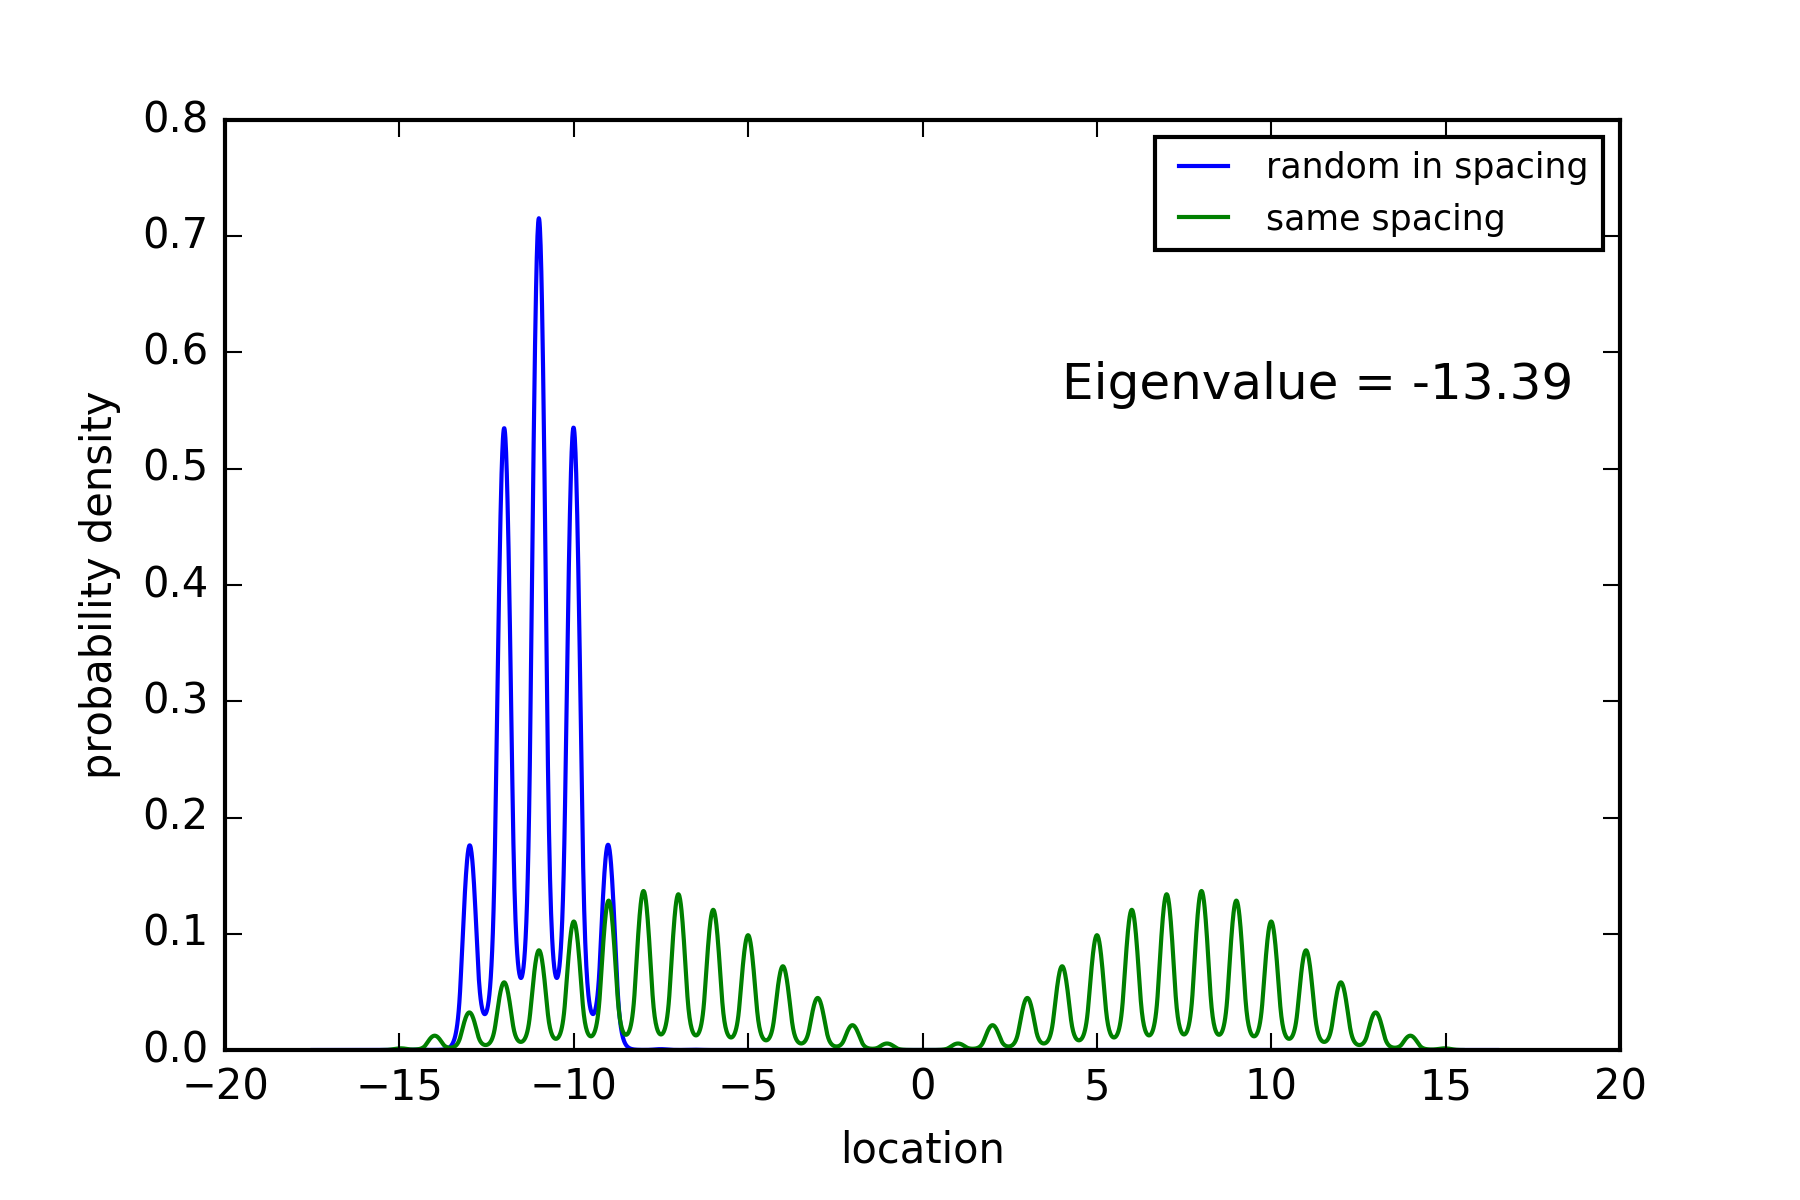
\includegraphics[width=1.1\linewidth]{Graphics/10_0_2th_Lowest_Rand1_5.png}
  \captionof{figure}{2nd Lowest eigenvalue, $V_0l=10.0$, $\{p_1,p_2\}=\{1.5,1.0\}$}
  \label{fig:Area10_2thlowestRand1.5}
\end{minipage}%
\end{figure}

%16:45 modifiled

\newpage
\subsection{Randomness in potential}\label{Randomness in potential}
Since the potential is determined in this model by the potential height and well width, and the product of potential height and well width gives the area of the square potential, we can introduce randomness to this type of system by fixing a value for the area first, and at each atom site, picking a value for the well width from $\{w_1,w_2\}$ with probability $\{0.5,0.5\}$.  For example, for a chain of 5 atoms, we might get a sequence of well widths, ${0.2,0.5,0.5,0.2,0.2}$ if we are allowed to pick from $\{0.2,0.5\}$. With area given, say 1.0, we are can get a sequence of potential heights for the atoms, {5,2,,2,5,5}. Hence these two sequences define the non-overlapping square potential at each atom site for this system of 5 atoms. 

The following figures are probability density function corresponding to first and second lowest eigenenergies when $V_0l$ is equal to 1 or 2 or 5, with well width picked from $\{w_1,w_2\}$ with probability of $\{0.5,0.5\}$.

%lowest vl = 1.0

\begin{figure}[!htbh]
\centering
\begin{minipage}{.45\textwidth}
  \centering
  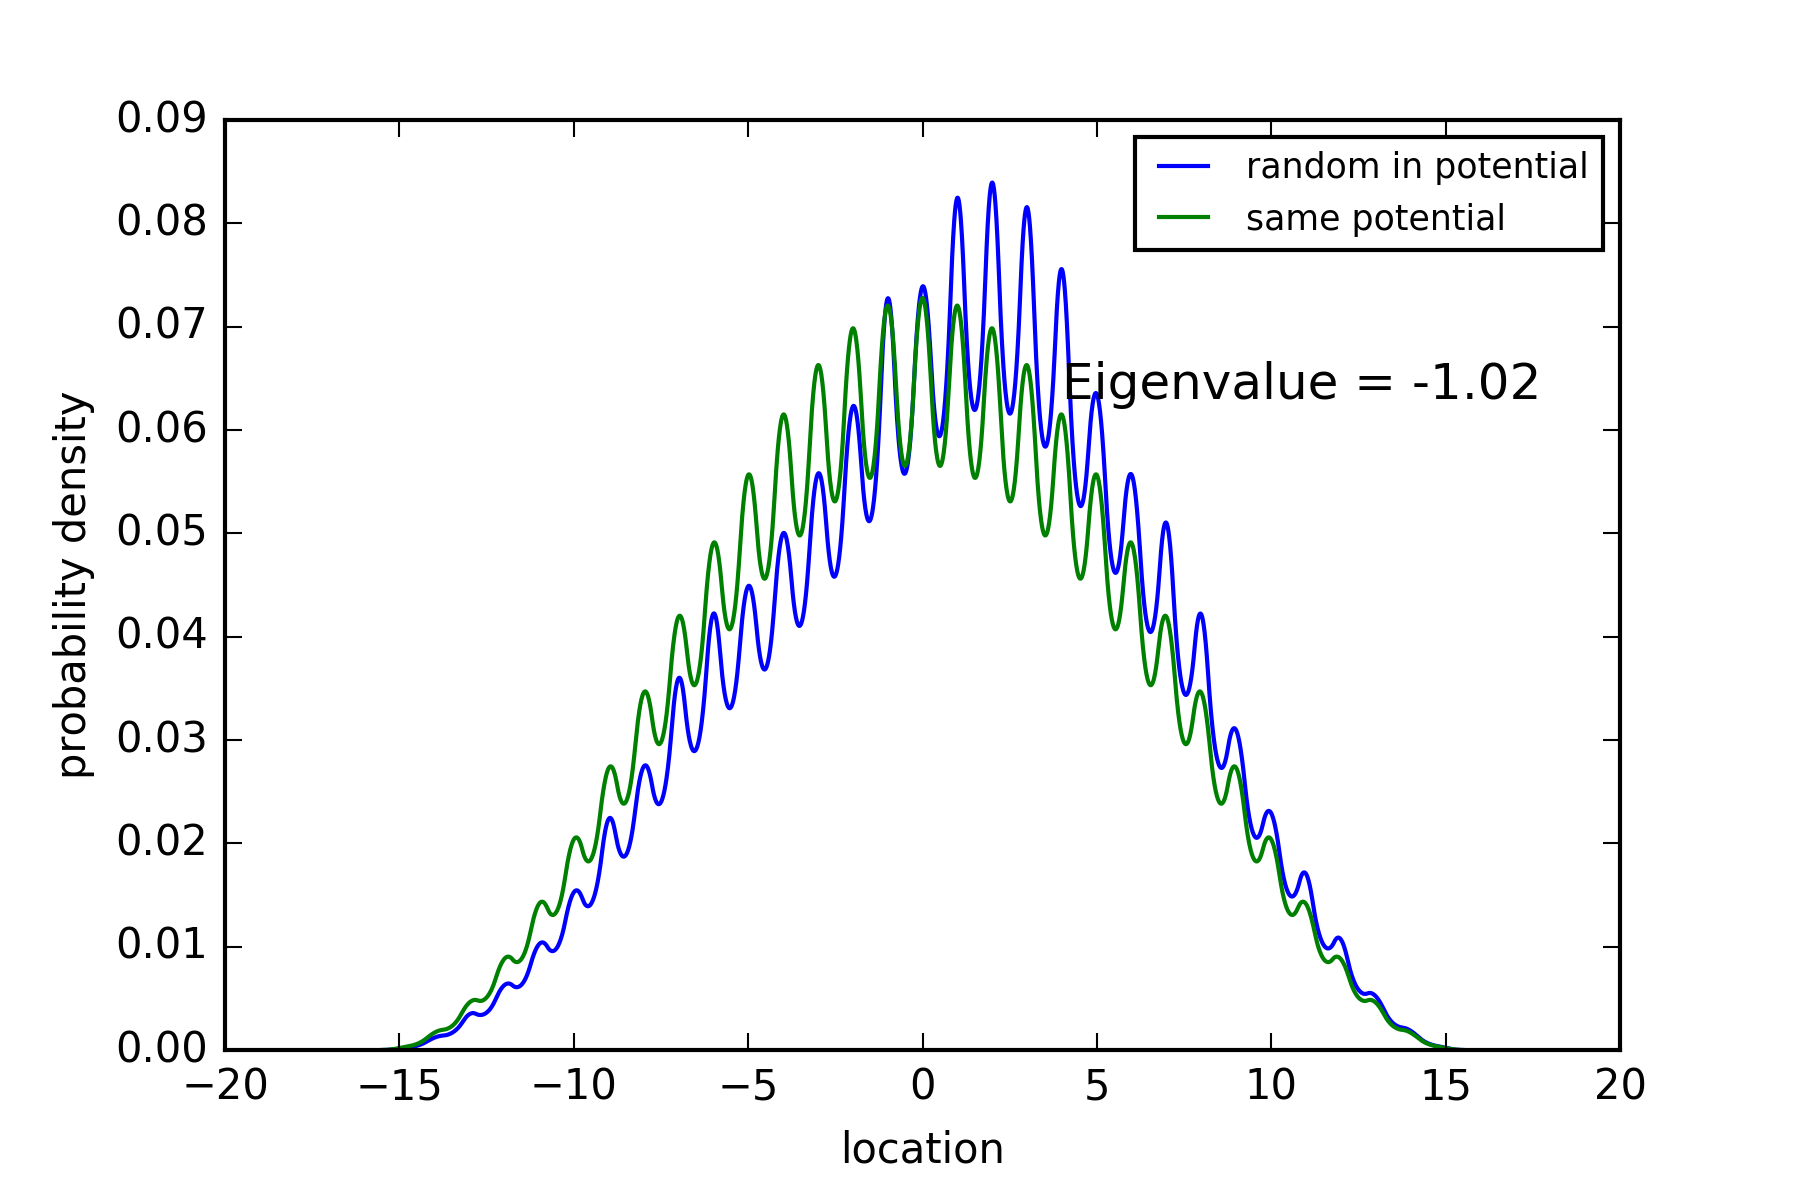
\includegraphics[width=1.1\linewidth]{RandomPotential2/1_0a_1th_Lowest_Rand0_4_0_5.png}
  \captionof{figure}{Lowest eigenvalue, $V_0l =1.0$ , $w_1 = 0.4 $,$w_2 = 0.5$ }
  \label{fig:randPoa1_1th_0.5_0.4}
\end{minipage}\qquad
\begin{minipage}{.45\textwidth}
  \centering
  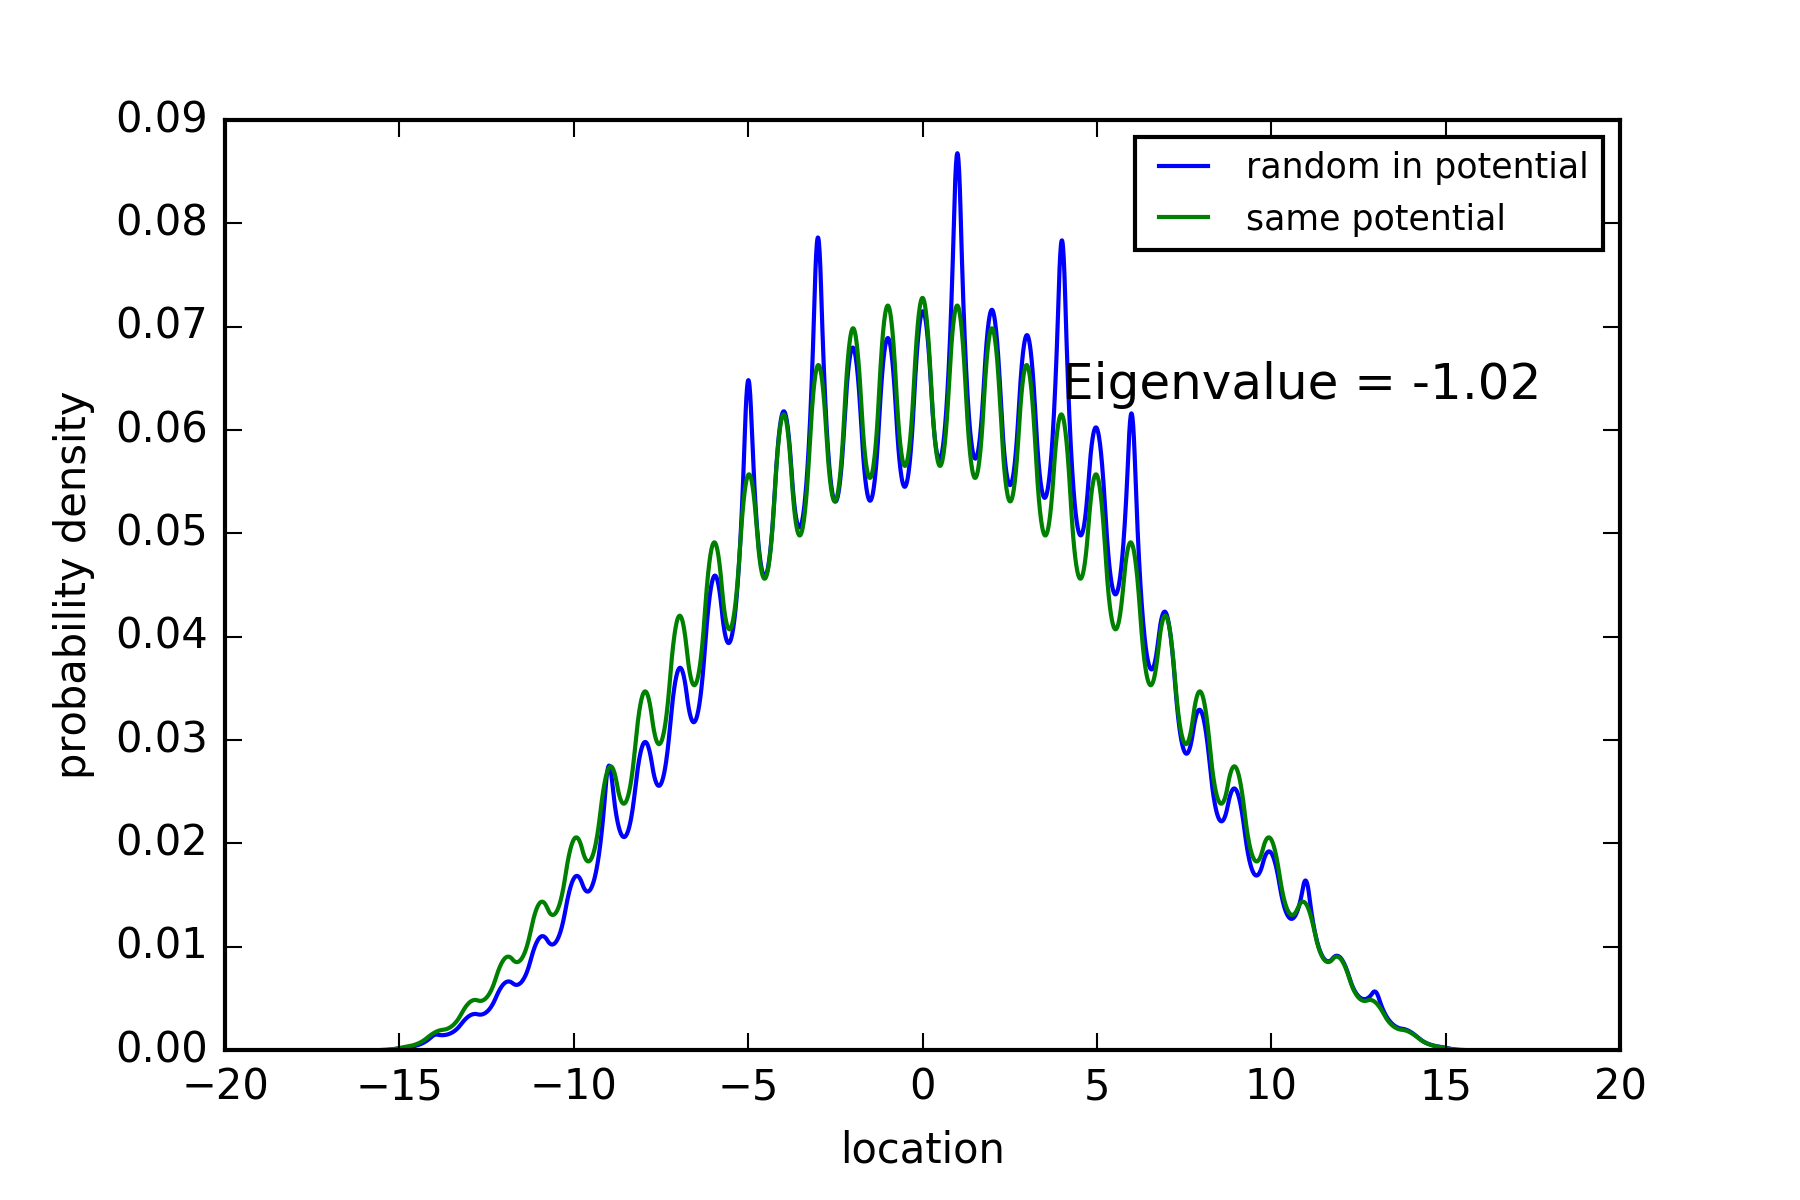
\includegraphics[width=1.1\linewidth]{RandomPotential2/1_0a_1th_Lowest_Rand0_2_0_5.png}
  \captionof{figure}{Lowest eigenvalue, $V_0l=1.0$, $w_1 = 0.2 $, $w_2 = 0.5 $}
  \label{fig:randPoa1_1th_0.5_0.2}
\end{minipage}
\end{figure}

%2nd lowest vl = 1.0
\begin{figure}[!htbh]
\centering
\begin{minipage}{.45\textwidth}
  \centering
  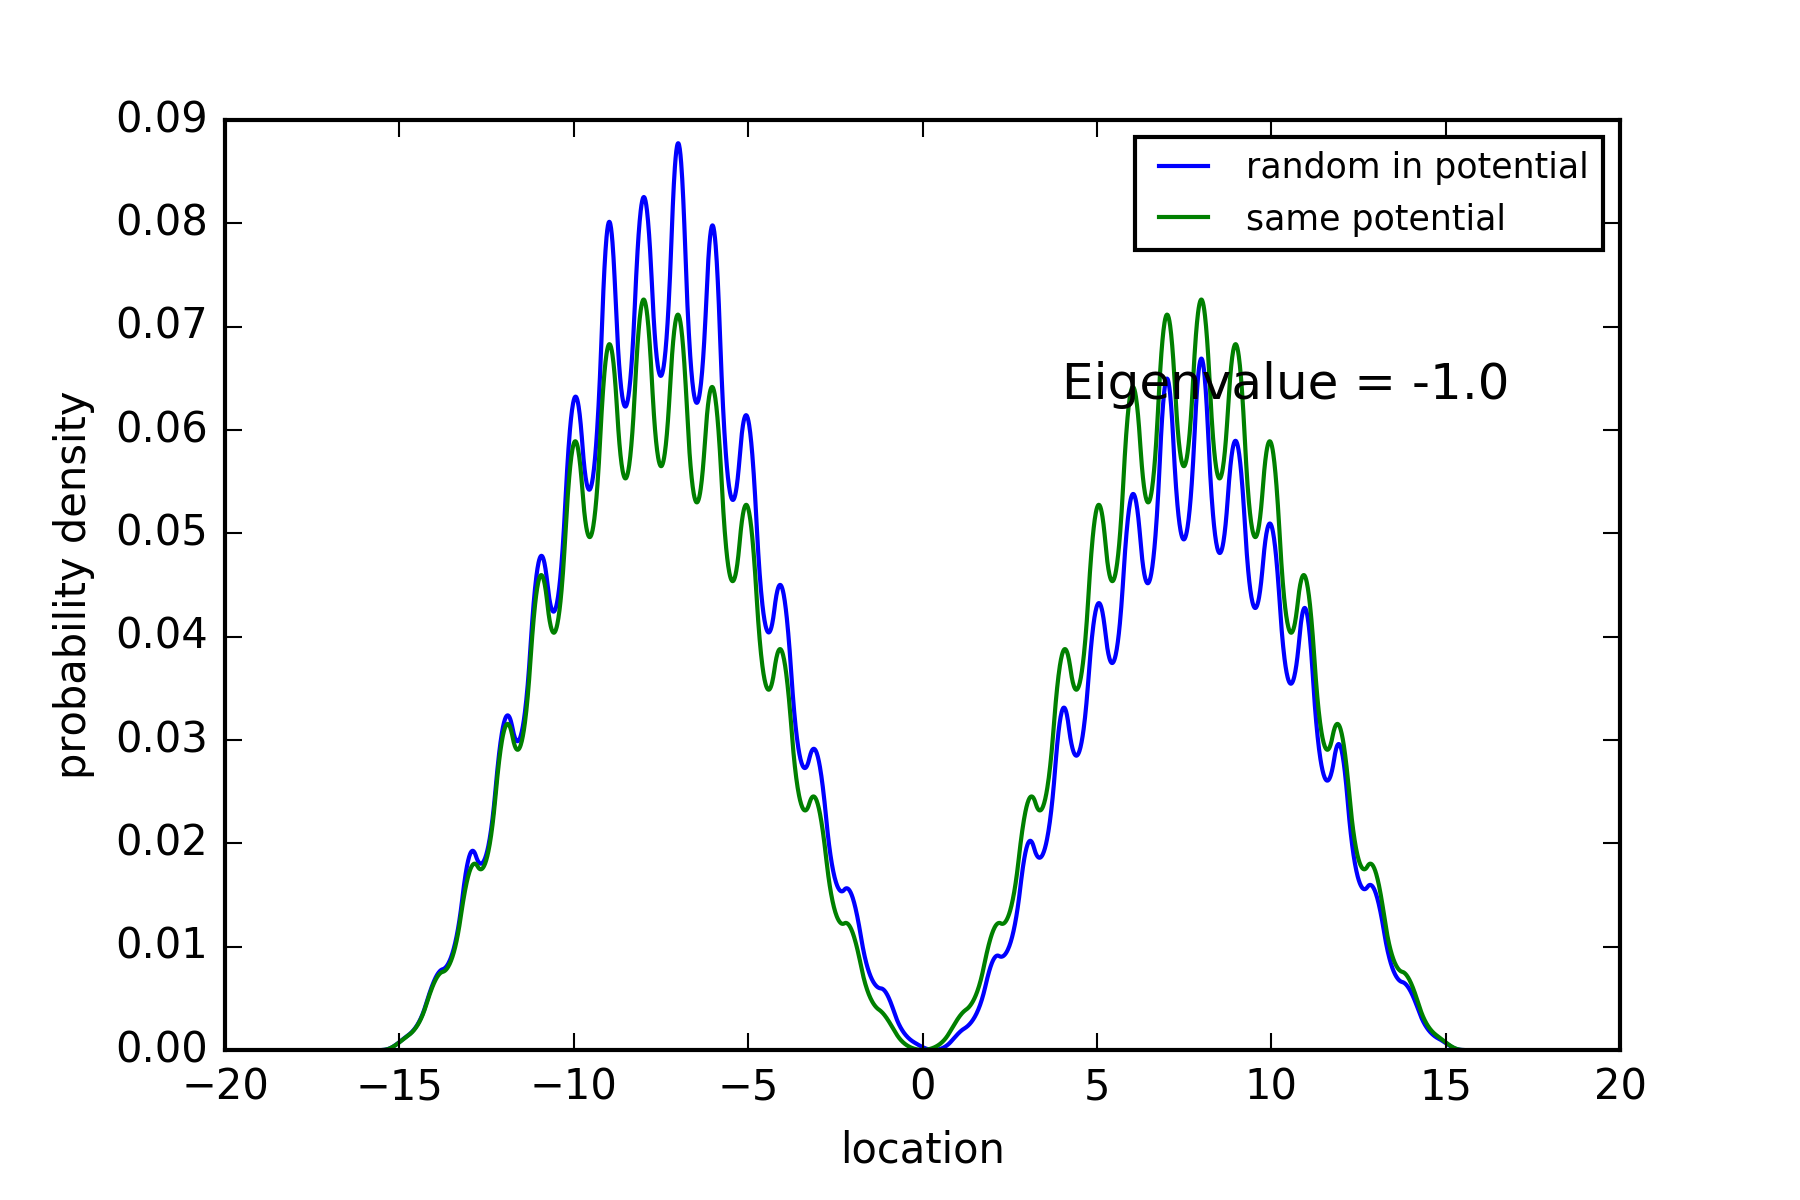
\includegraphics[width=1.1\linewidth]{RandomPotential2/1_0a_2th_Lowest_Rand0_4_0_5.png}
  \captionof{figure}{Lowest eigenvalue $V_0l$=1.0, $w_1 = 0.4 $,$w_2 = 0.5$}
  \label{fig:randPoa1_2th_0.5_0.4}
\end{minipage}\qquad
\begin{minipage}{.45\textwidth}
  \centering
  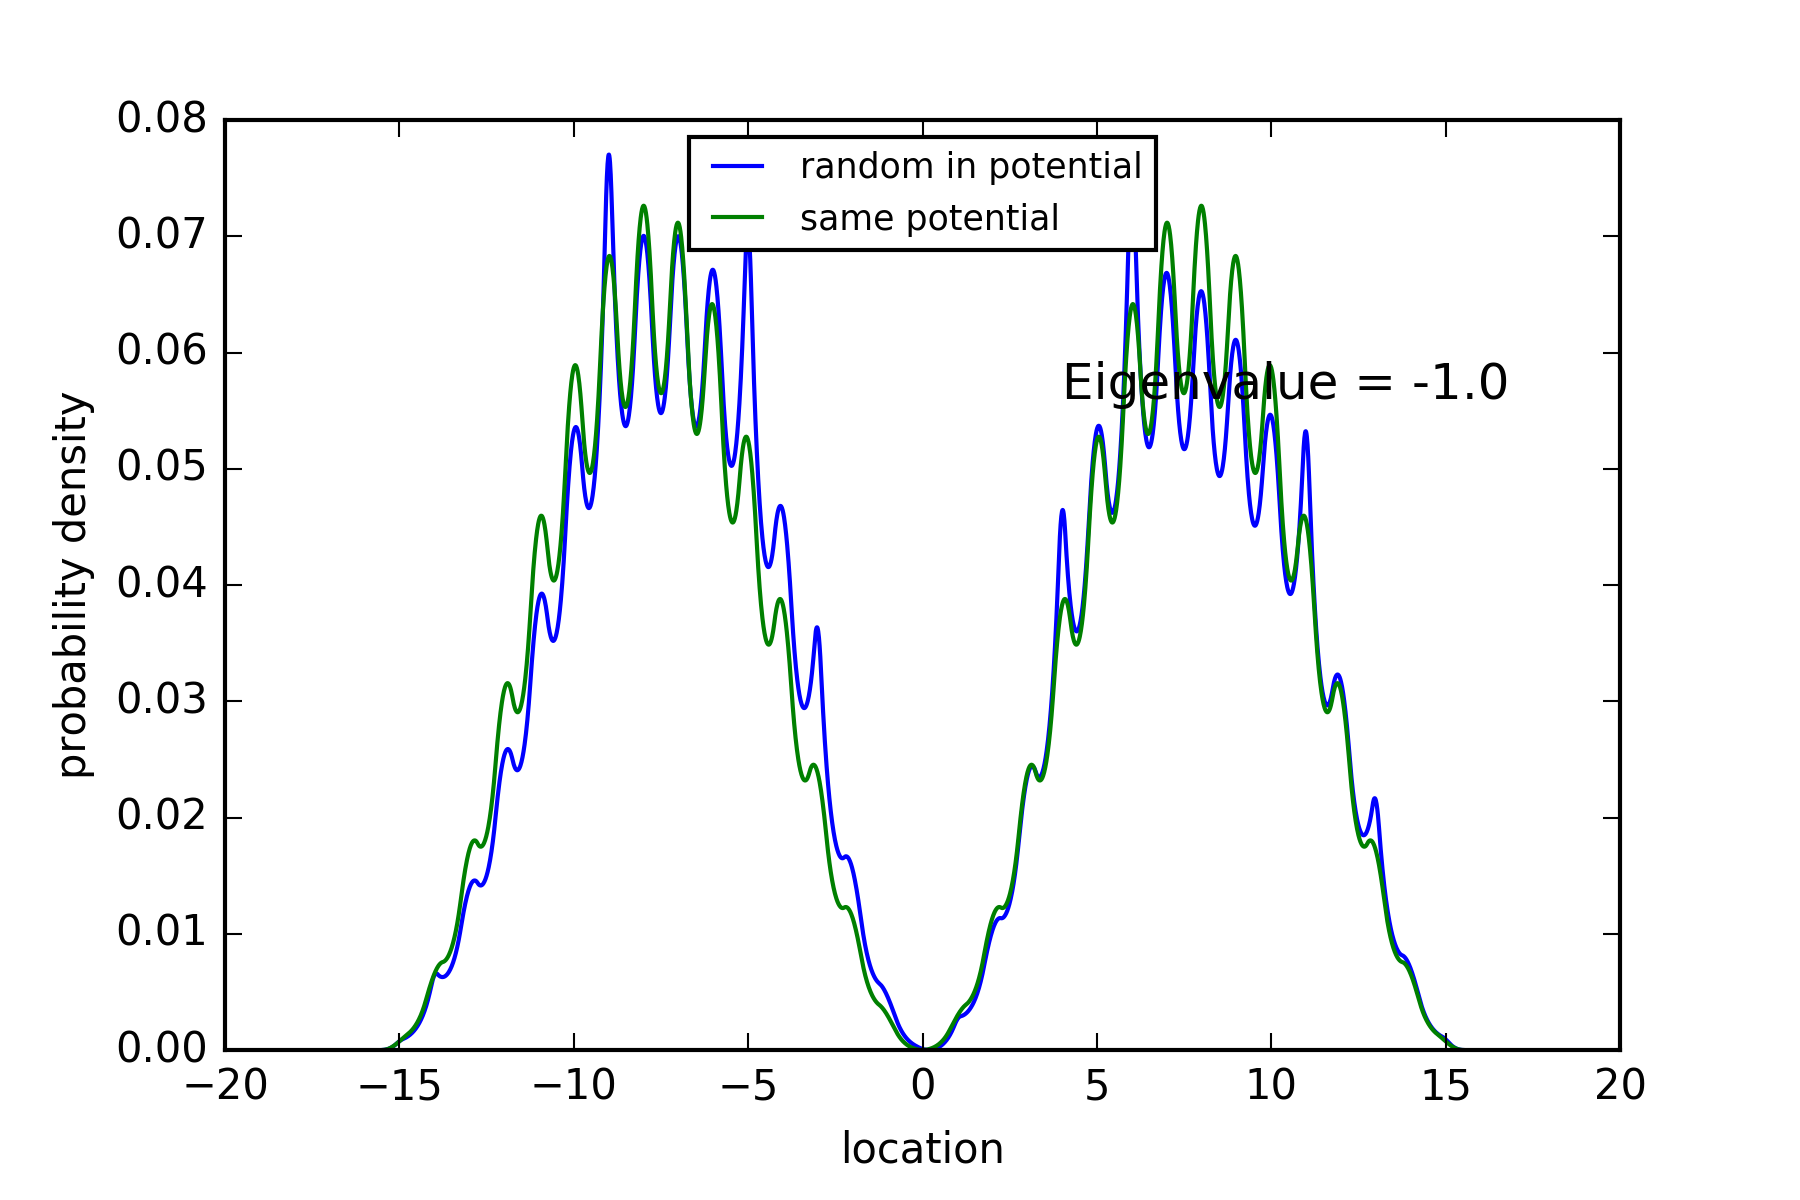
\includegraphics[width=1.1\linewidth]{RandomPotential2/1_0a_2th_Lowest_Rand0_2_0_5.png}
  \captionof{figure}{Lowest eigenvalue, $V_0l=1.0$,$w_1 = 0.2 $, $w_2 = 0.5 $}
  \label{fig:randPoa1_2th_0.5_0.4}
\end{minipage}
\end{figure}

%lowest vl = 5.0
\begin{figure}[!htbh]
\centering
\begin{minipage}{.45\textwidth}
  \centering
  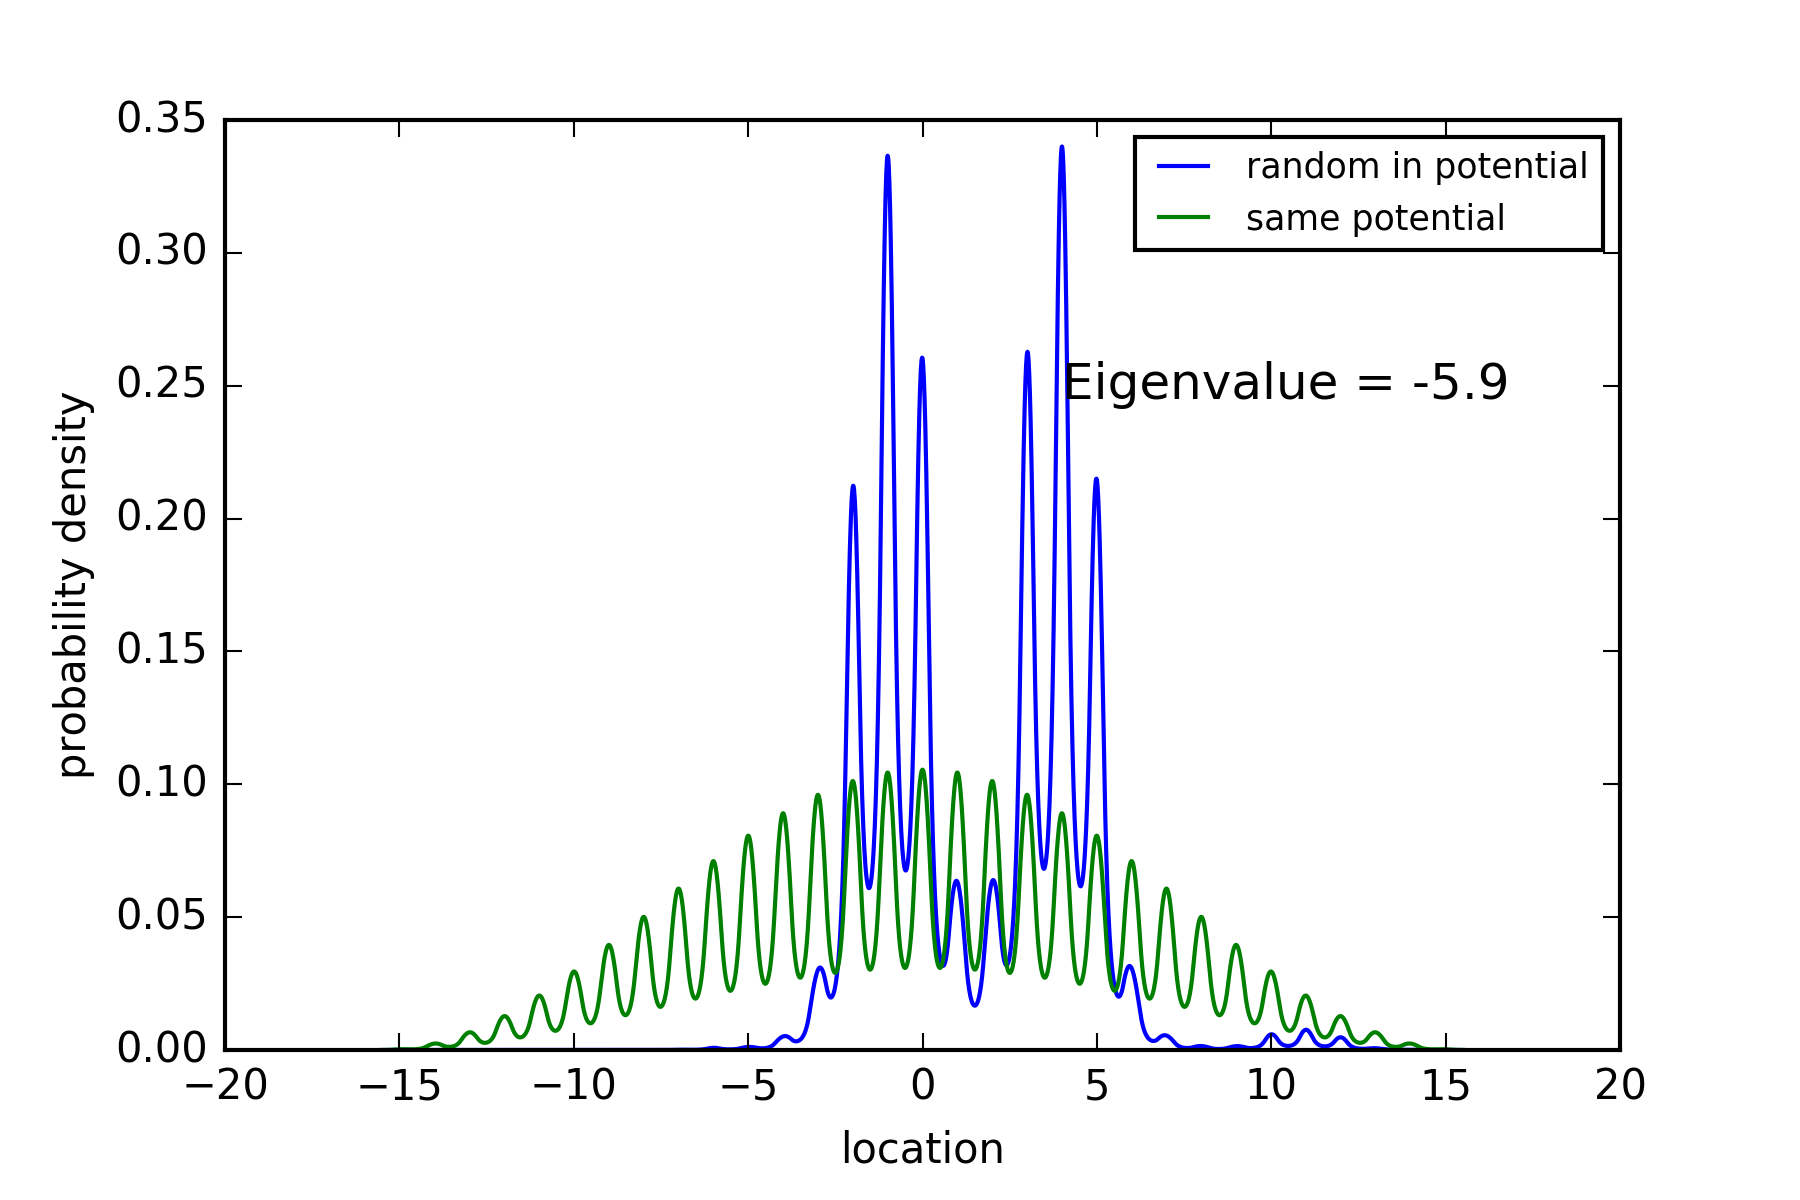
\includegraphics[width=1.1\linewidth]{RandomPotential2/5_0a_1th_Lowest_Rand0_4_0_5.png}
  \captionof{figure}{Lowest eigenvalue $V_0l=5.0$, $w_1 = 0.4 $,$w_2 = 0.5$}
  \label{fig:randPoa5_1th_0.5_0.4}
\end{minipage}\qquad
\begin{minipage}{.45\textwidth}
  \centering
  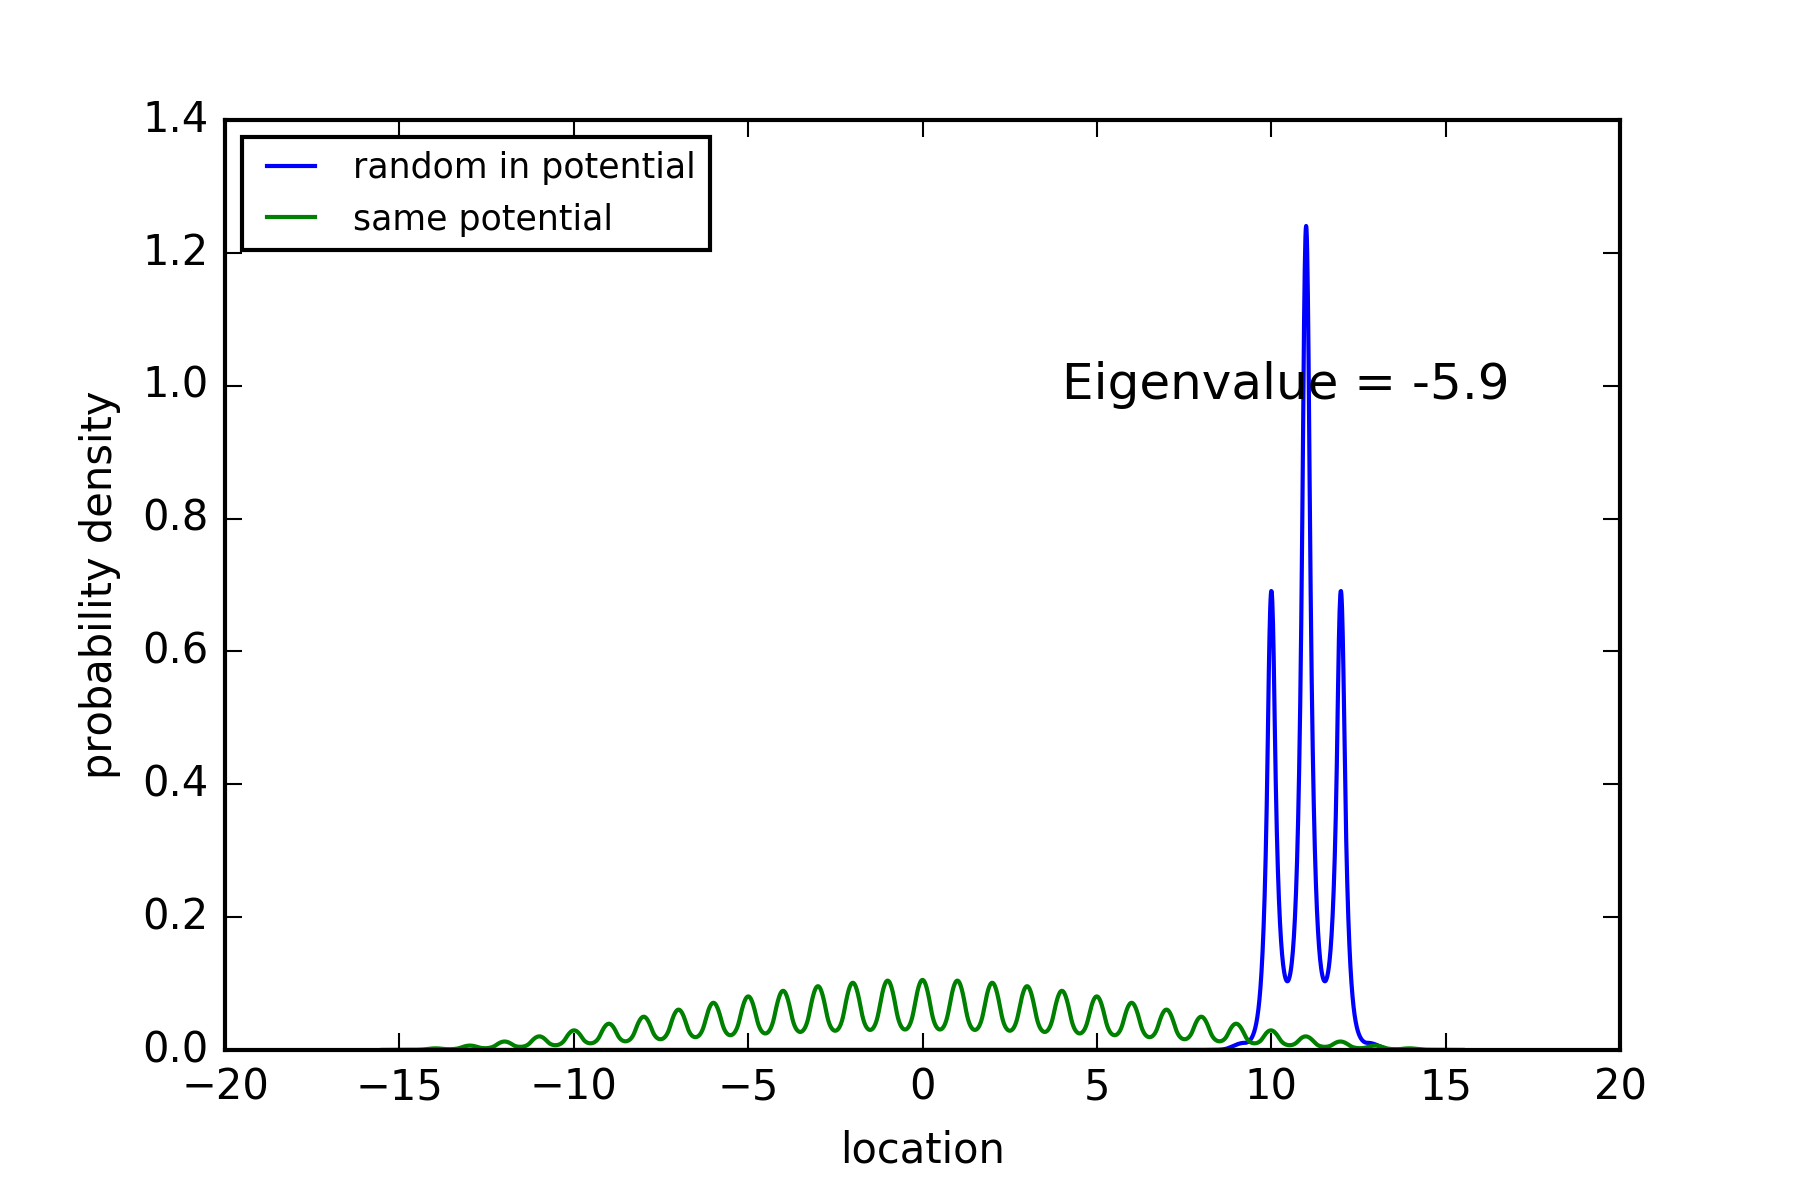
\includegraphics[width=1.1\linewidth]{RandomPotential2/5_0a_1th_Lowest_Rand0_2_0_5.png}
  \captionof{figure}{Lowest eigenvalue $V_0l=5.0$, $w_1 = 0.2 $, $w_2 = 0.5 $}
  \label{fig:randPoa5_1th_0.5_0.2}
\end{minipage}
\end{figure}

%2nd lowest vl = 5.0
\begin{figure}[!htbh]
\centering
\begin{minipage}{.45\textwidth}
  \centering
  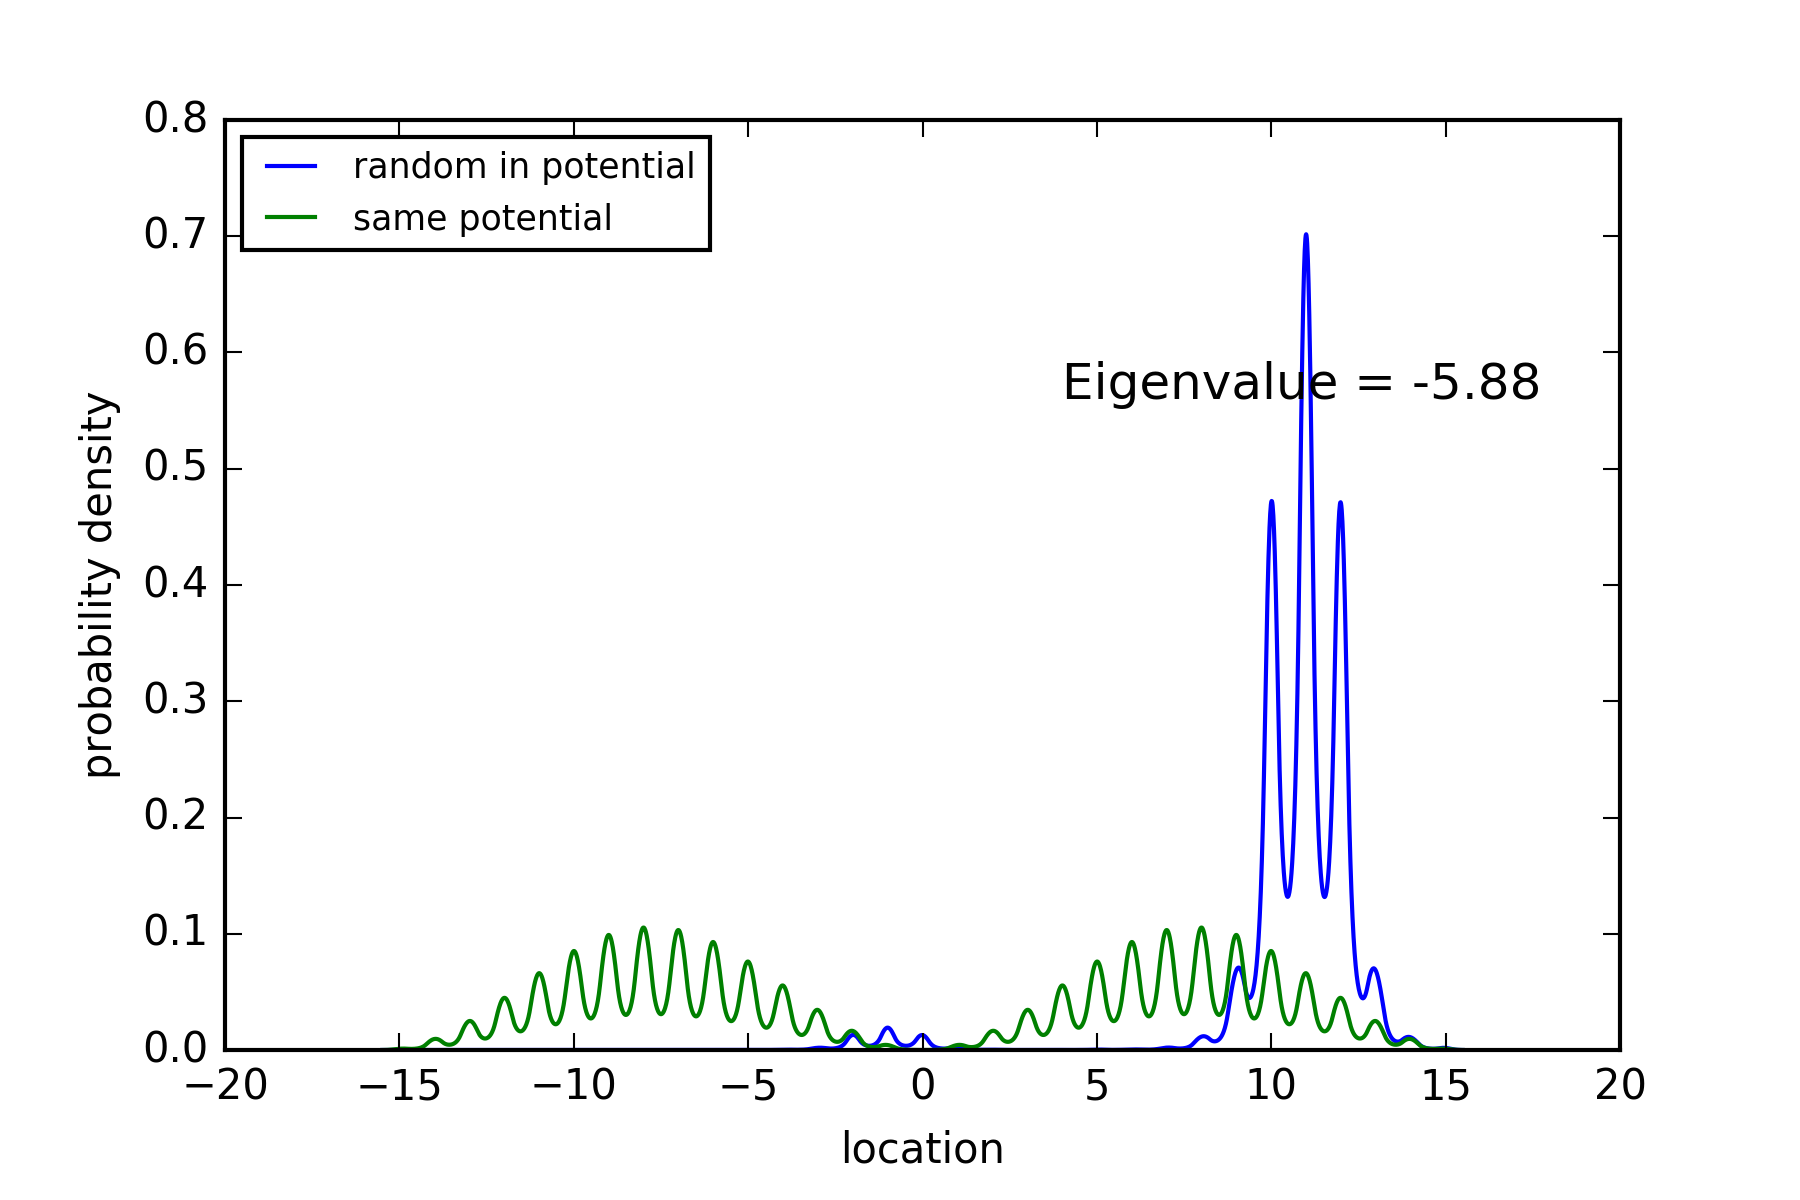
\includegraphics[width=1.1\linewidth]{RandomPotential2/5_0a_2th_Lowest_Rand0_4_0_5.png}
  \captionof{figure}{2nd Lowest eigenvalue, $V_0l=5.0$, $w_1 = 0.4 $,$w_2 = 0.5$}
  \label{fig:randPoa5_2th_0.5_0.4}
\end{minipage}\qquad
\begin{minipage}{.45\textwidth}
  \centering
  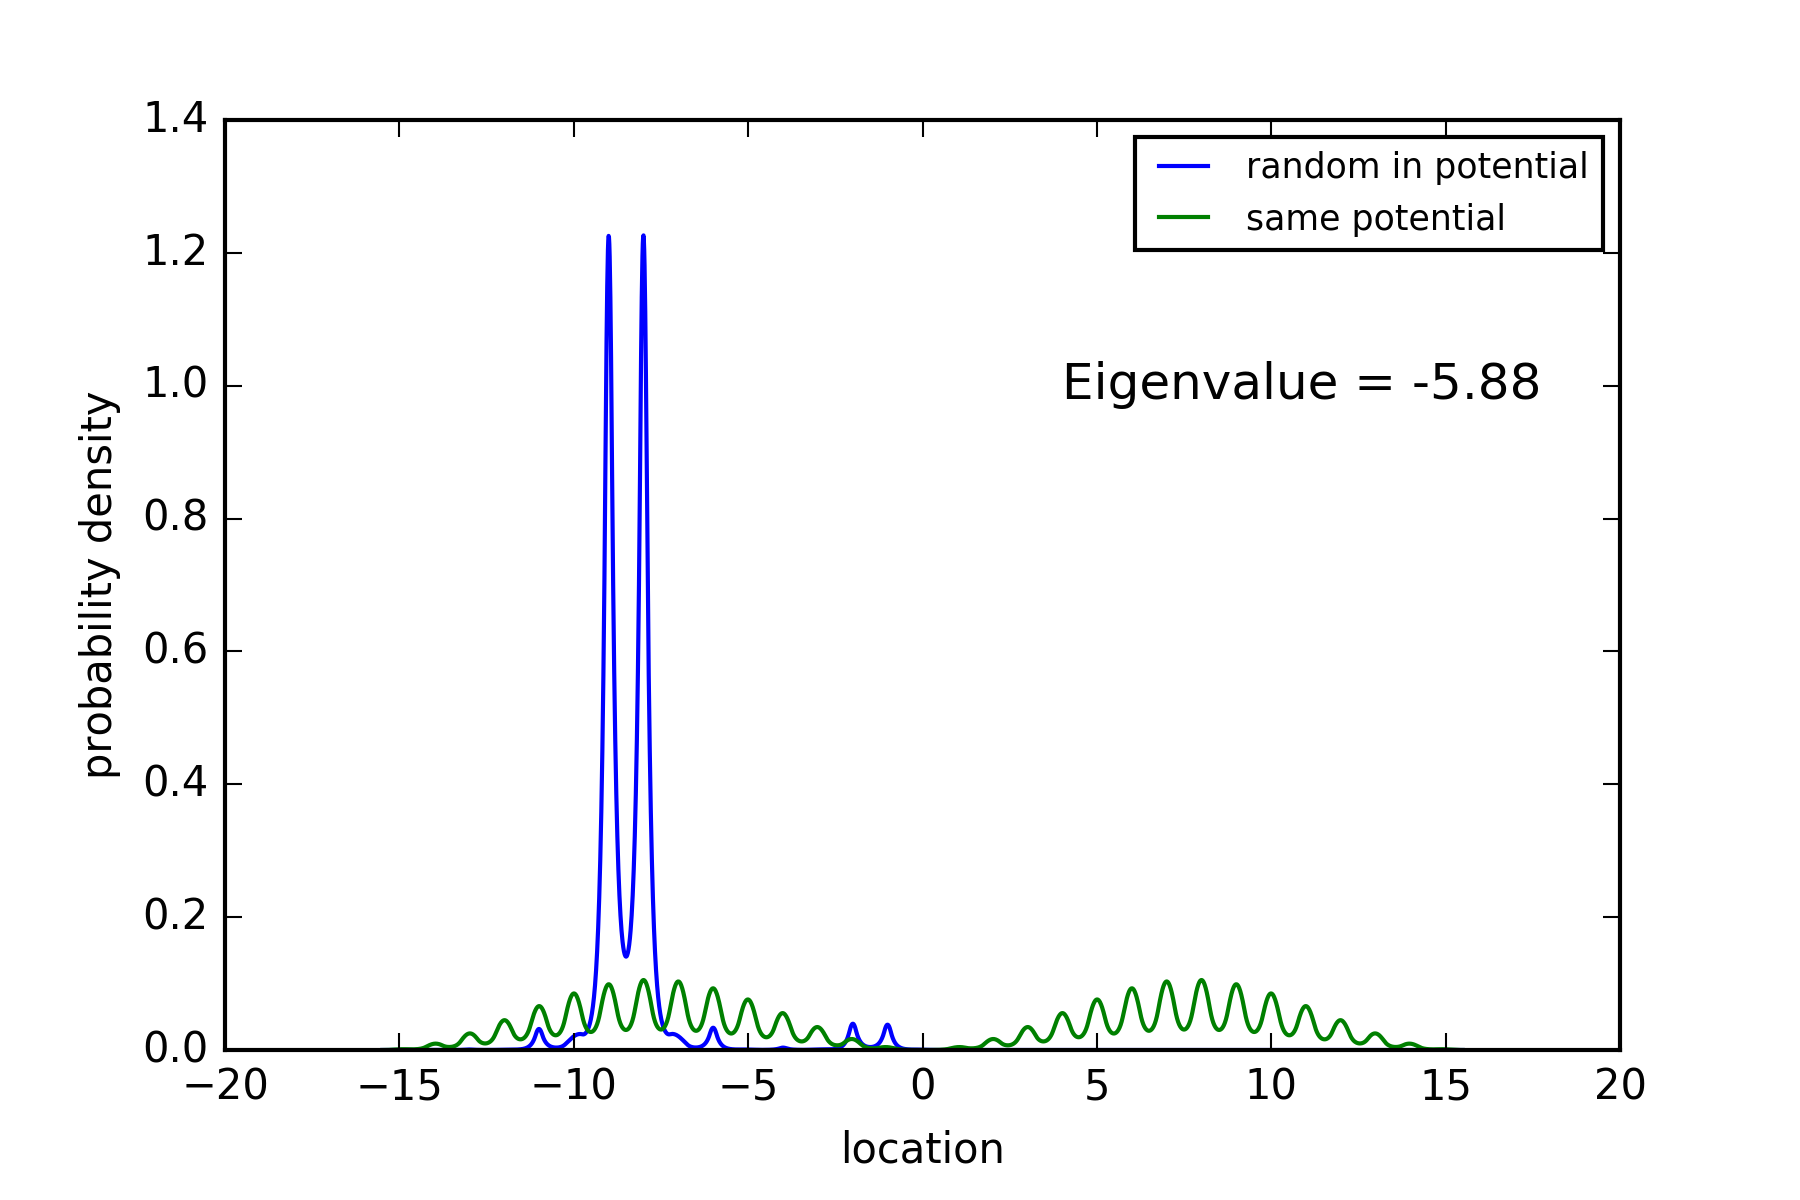
\includegraphics[width=1.1\linewidth]{RandomPotential2/5_0a_2th_Lowest_Rand0_2_0_5.png}
  \captionof{figure}{2nd Lowest eigenvalue, $V_0l=5.0$, $w_1 = 0.2 $, $w_2 = 0.5 $}
  \label{fig:randPoa5_2th_0.5_0.2}
\end{minipage}
\end{figure}

\newpage
%lowest vl = 10.0
\begin{figure}[!htbh]
\centering
\begin{minipage}{.45\textwidth}
  \centering
  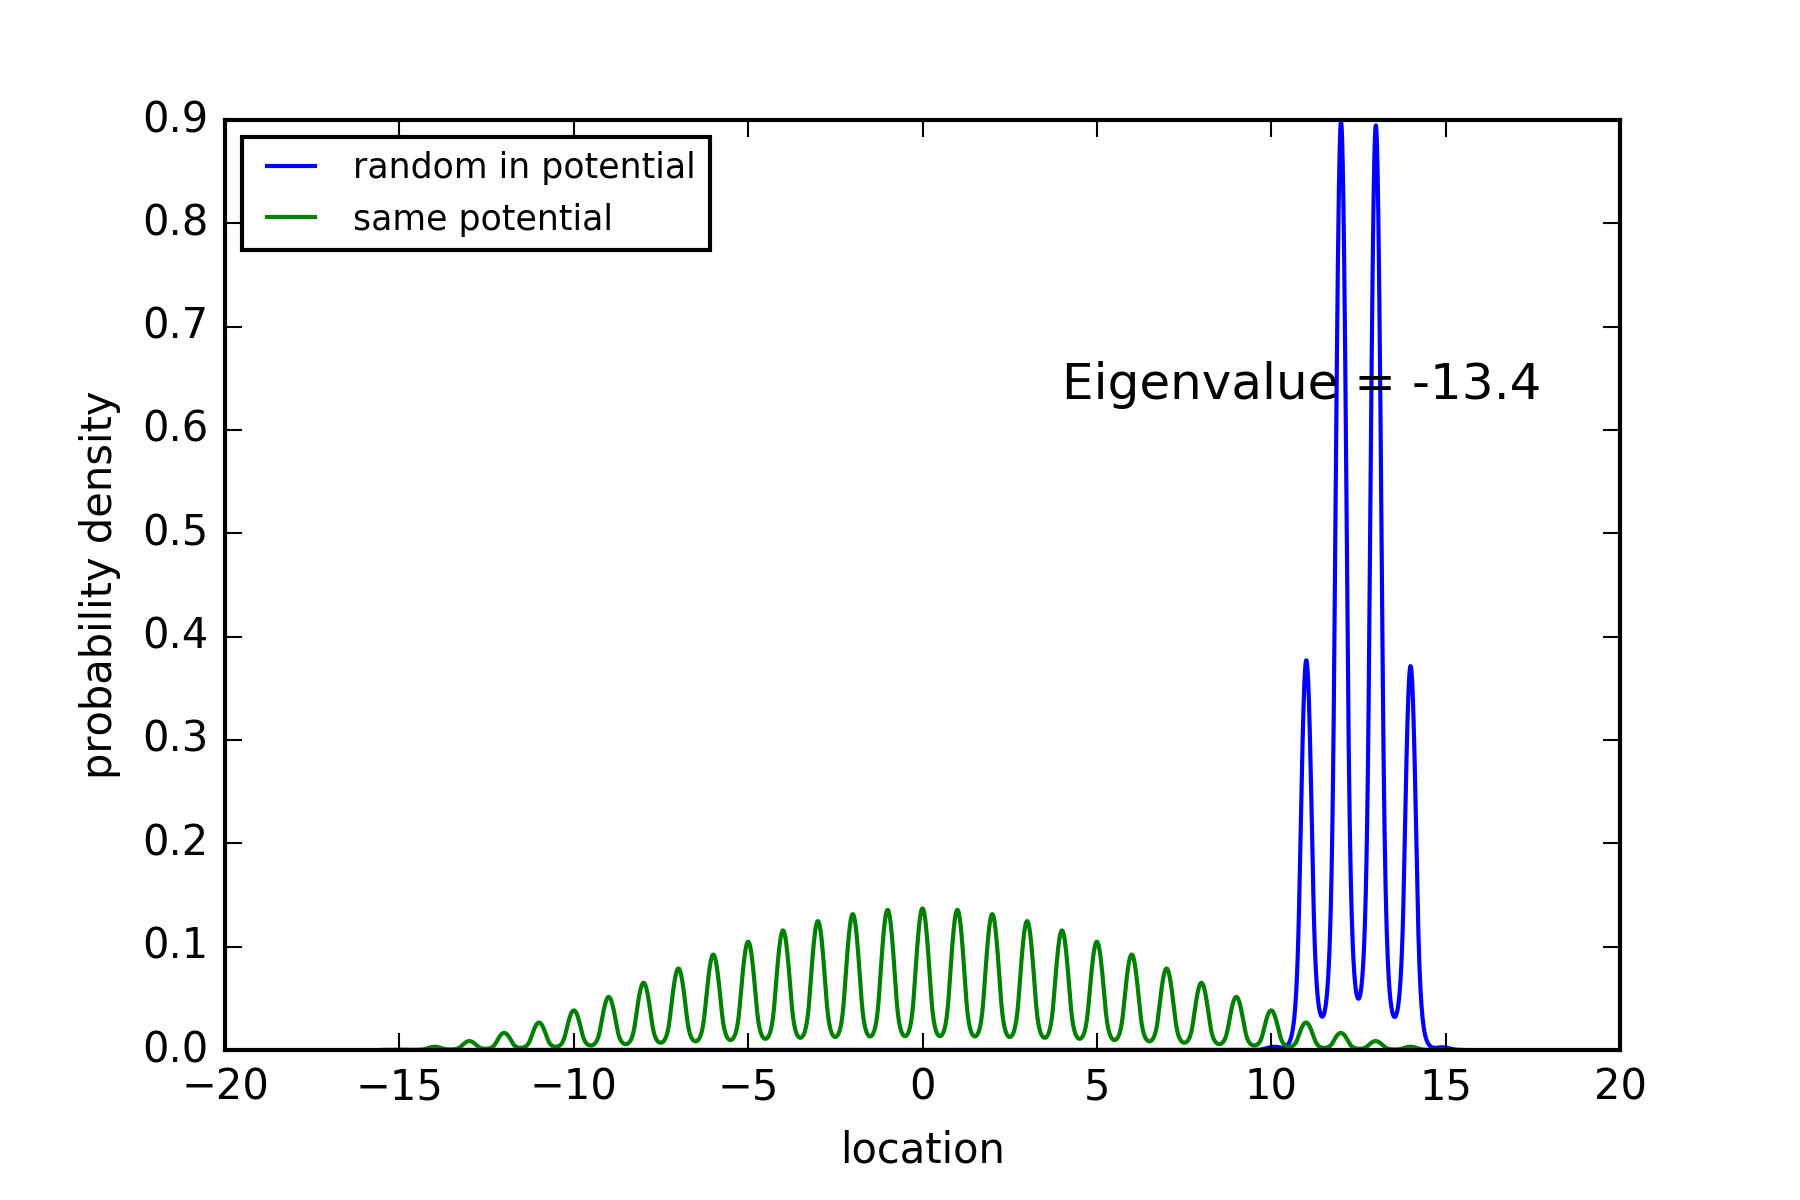
\includegraphics[width=1.1\linewidth]{RandomPotential2/10_0a_1th_Lowest_Rand0_4_0_5.png}
  \captionof{figure}{Lowest eigenvalue, $V_0l=10.0$, $w_1 = 0.4 $,$w_2 = 0.5$}
  \label{fig:randPoa10_1th_0.5_0.4}
\end{minipage}\qquad
\begin{minipage}{.45\textwidth}
  \centering
  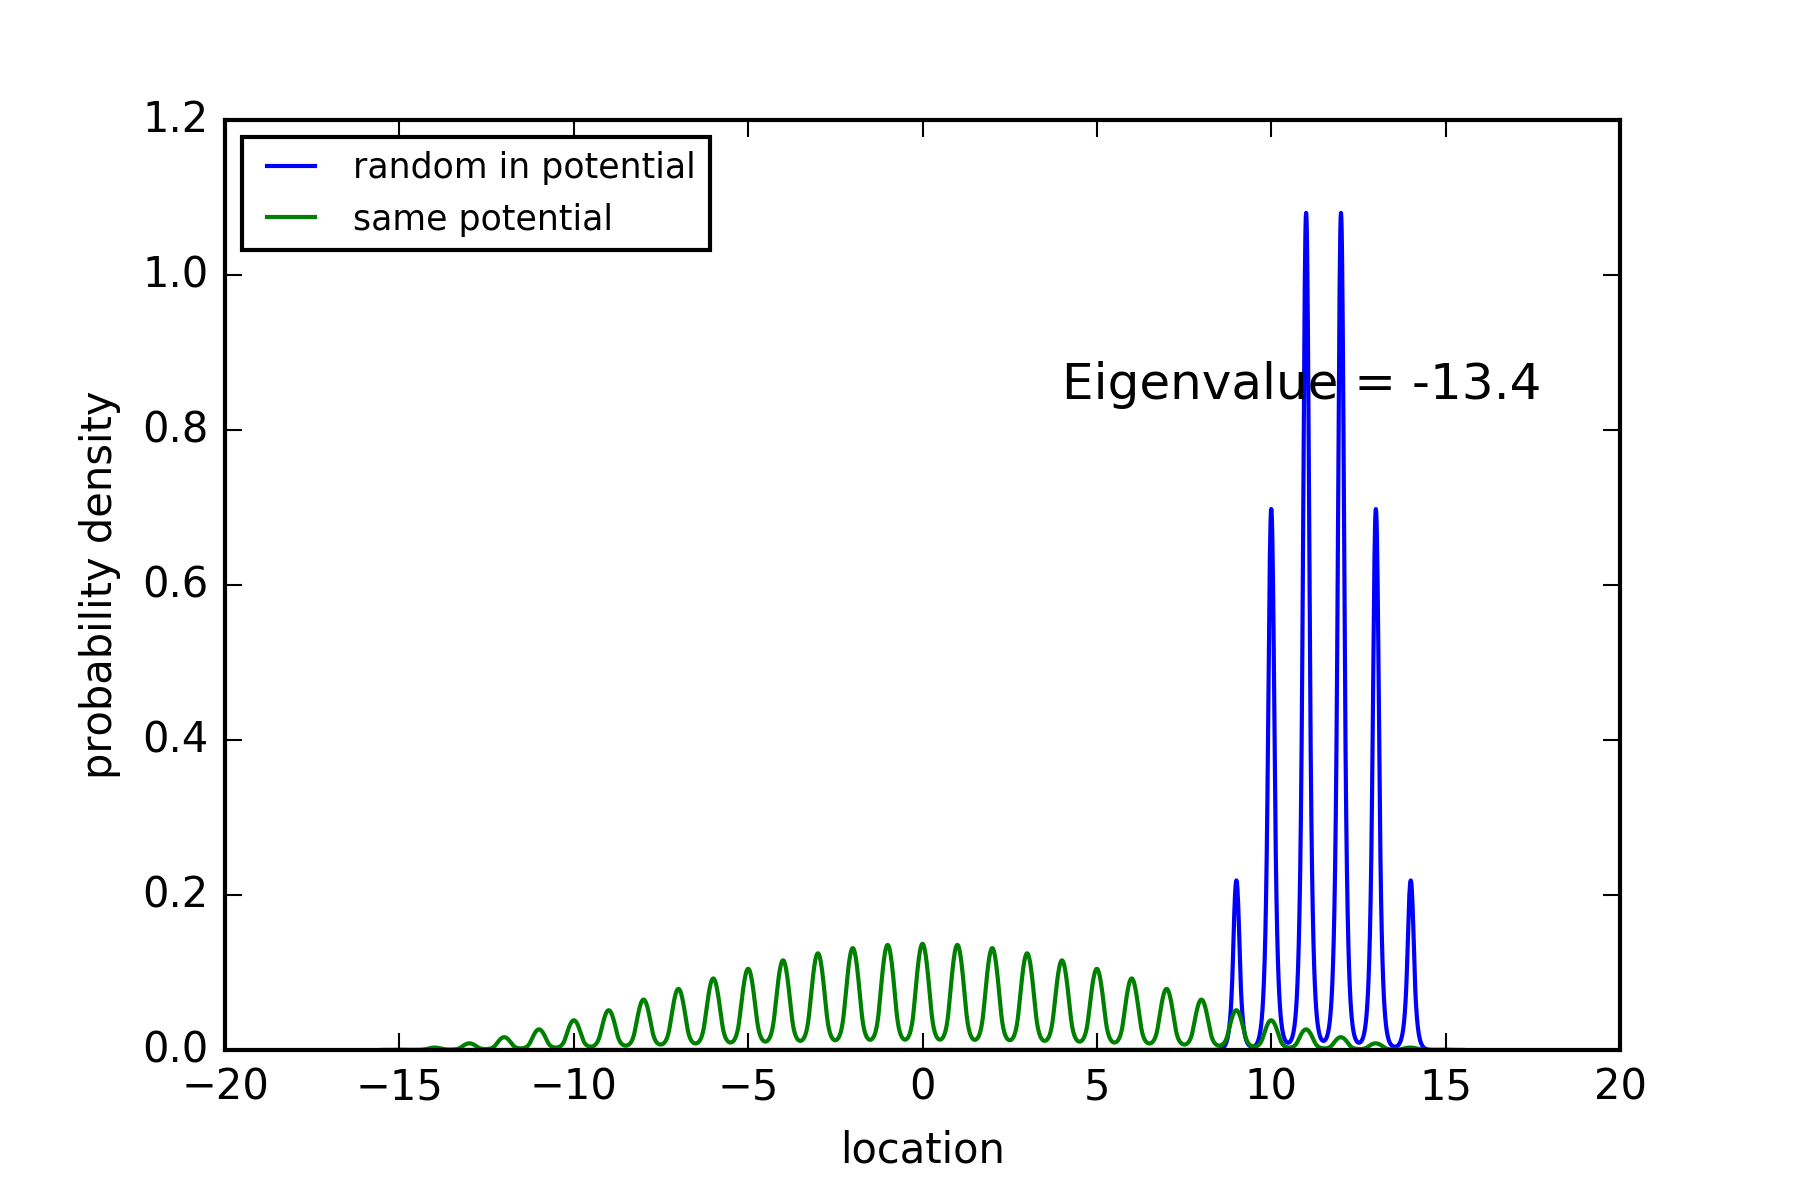
\includegraphics[width=1.1\linewidth]{RandomPotential2/10_0a_1th_Lowest_Rand0_2_0_5.png}
  \captionof{figure}{Lowest eigenvalue, $V_0l=10.0$, $w_1 = 0.2 $, $w_2 = 0.5 $}
  \label{fig:randPoa10_1th_0.5_0.2}
\end{minipage}
\end{figure}

%2nd lowest vl = 10.0
\begin{figure}[!htbh]
\centering
\begin{minipage}{.45\textwidth}
  \centering
  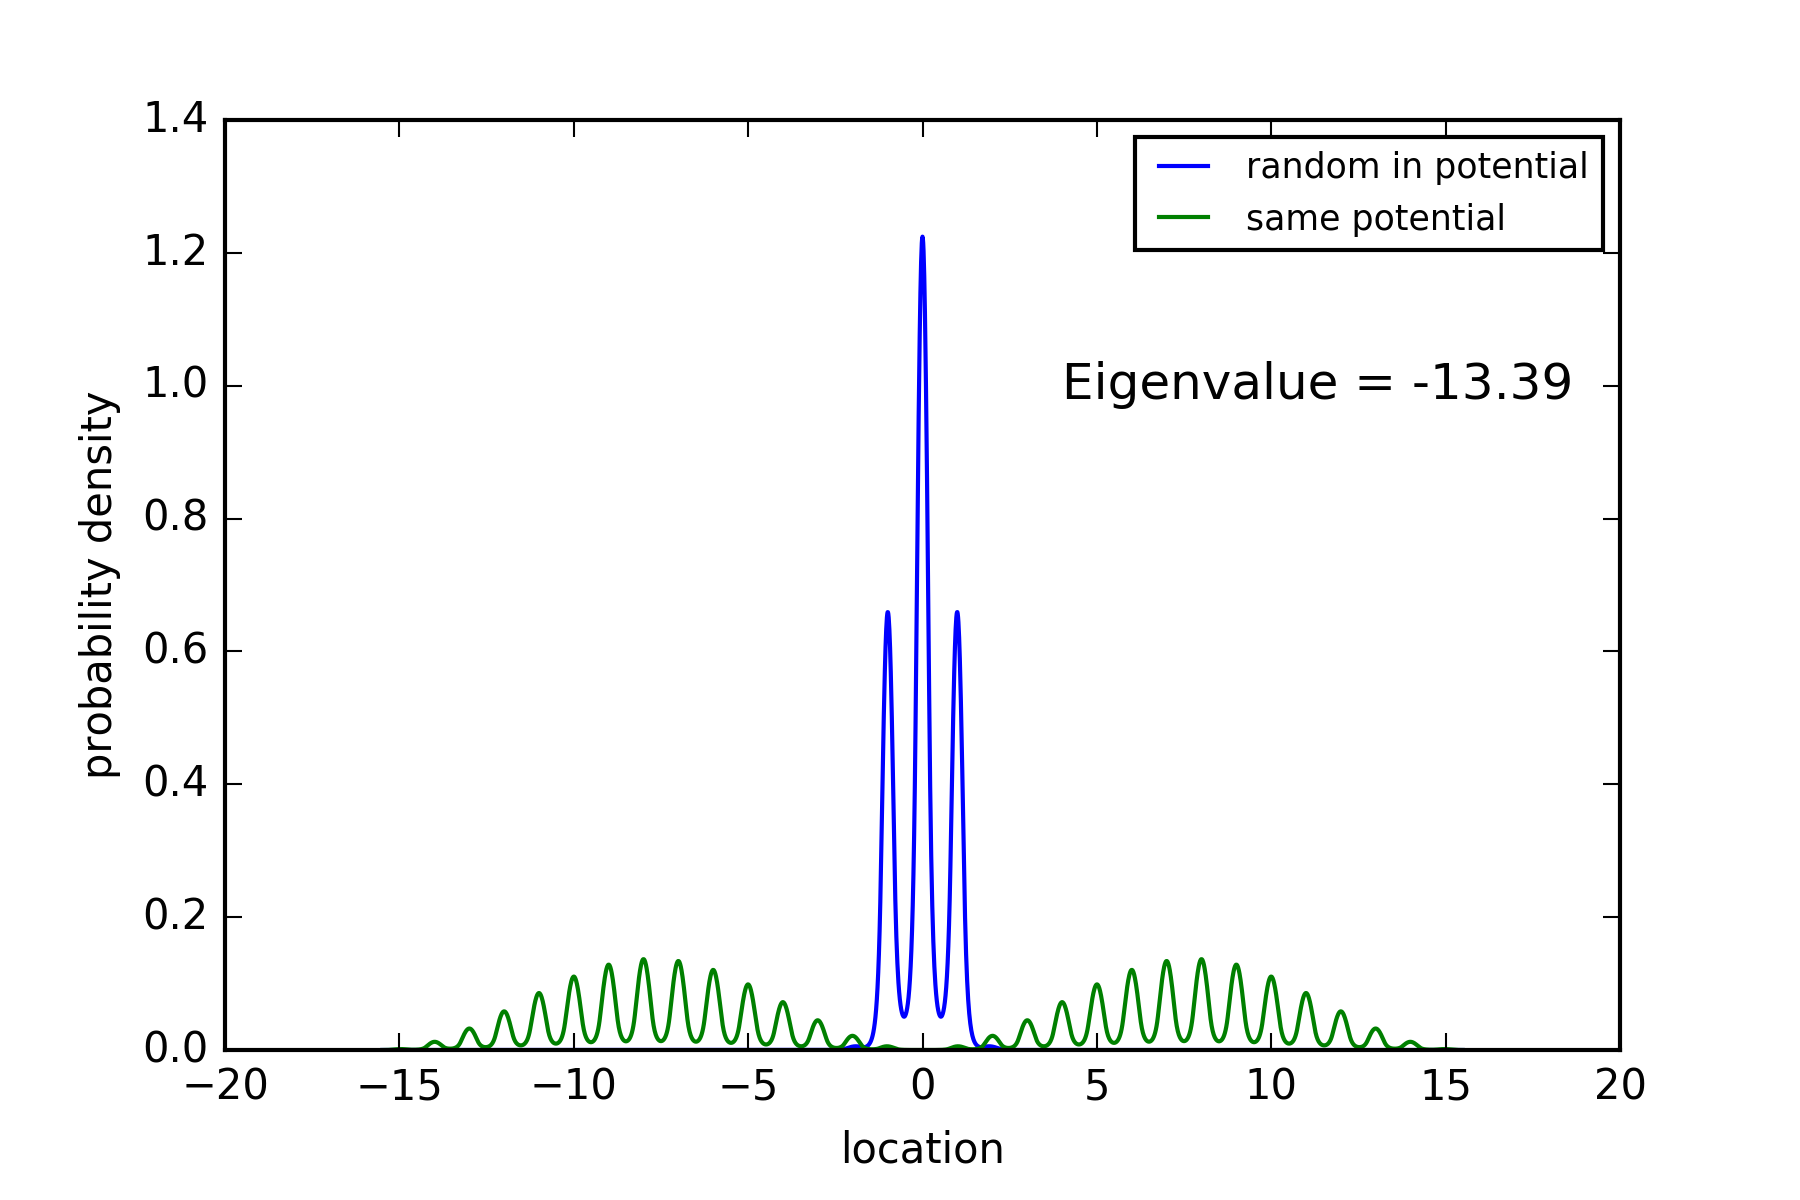
\includegraphics[width=1.1\linewidth]{RandomPotential2/10_0a_2th_Lowest_Rand0_4_0_5.png}
  \captionof{figure}{2nd Lowest eigenvalue, $V_0l =10.0$, $w_1 = 0.4 $,$w_2 = 0.5$}
  \label{fig:randPoa10_2th_0.5_0.4}
\end{minipage}\qquad
\begin{minipage}{.45\textwidth}
  \centering
  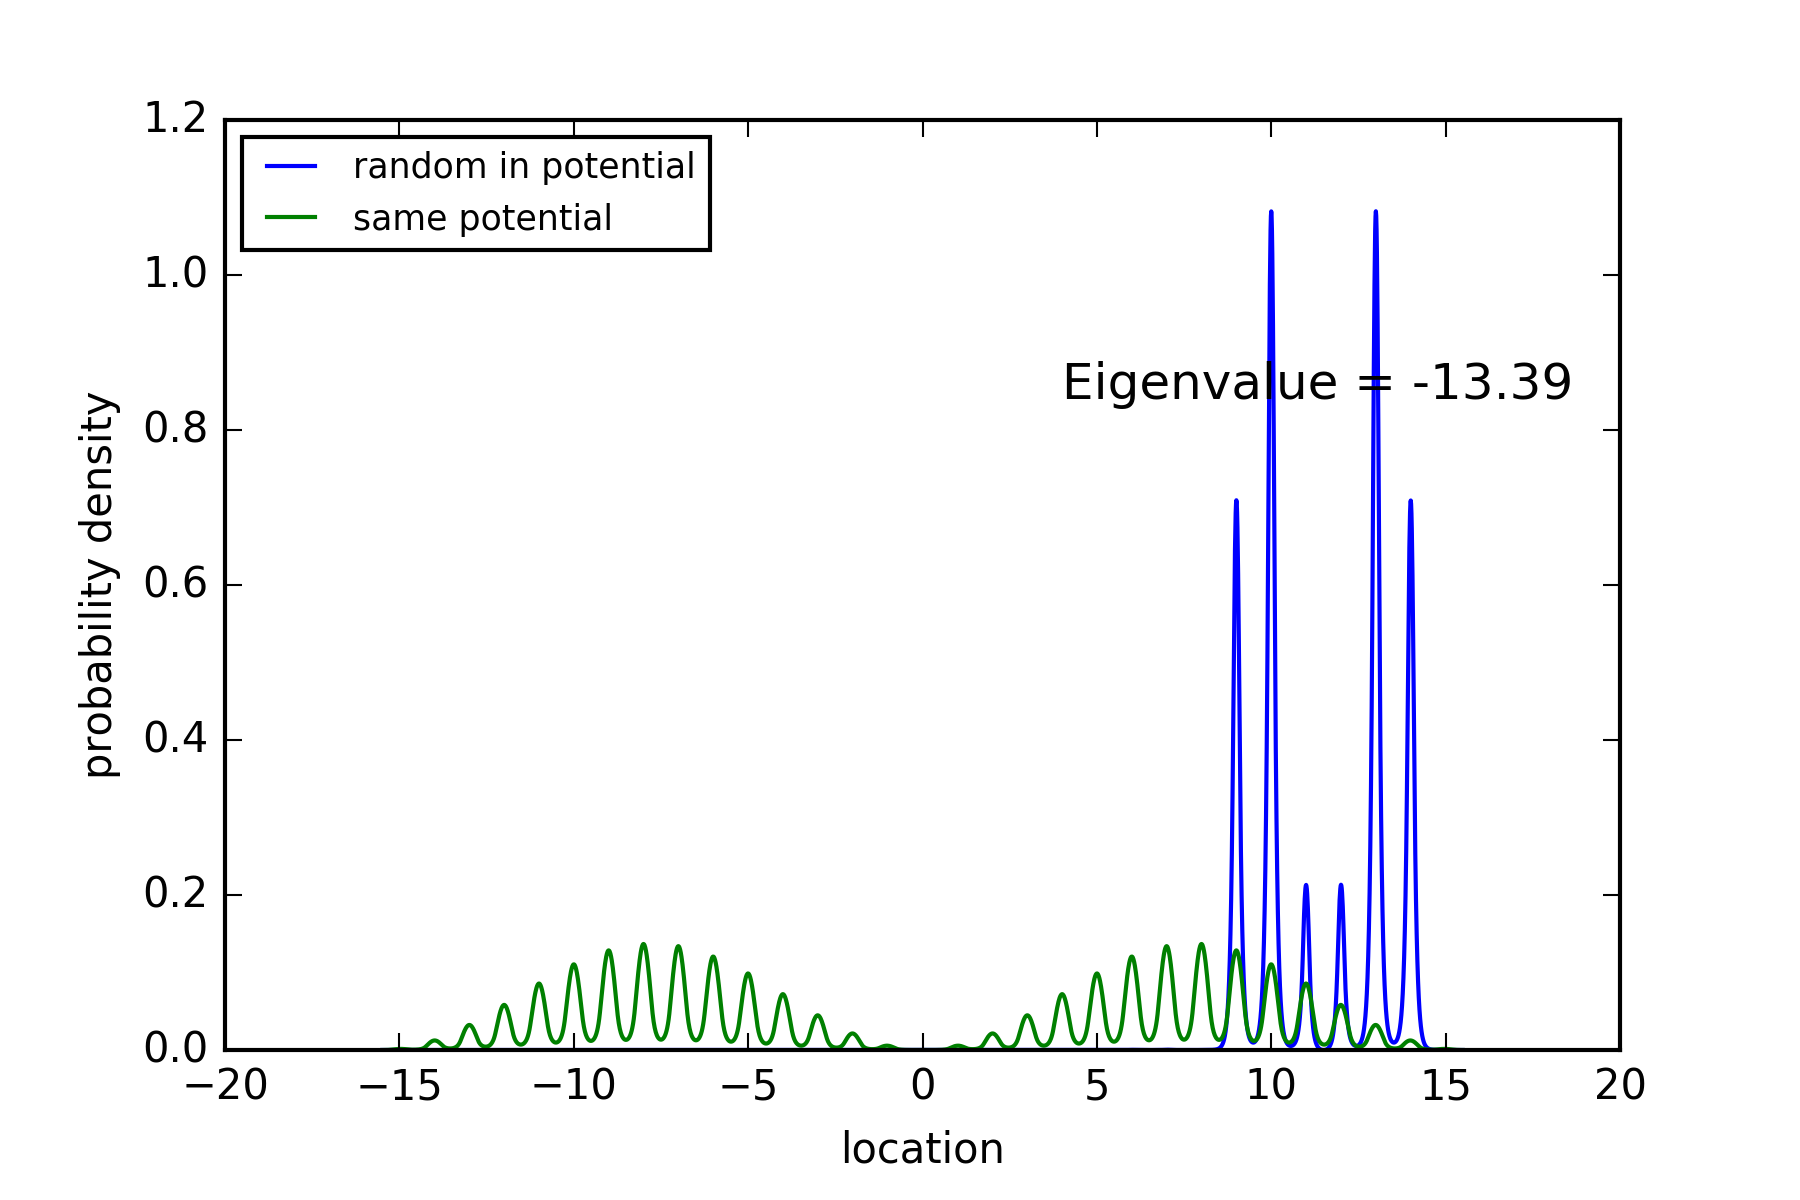
\includegraphics[width=1.1\linewidth]{RandomPotential2/10_0a_2th_Lowest_Rand0_2_0_5.png}
  \captionof{figure}{2nd Lowest eigenvalue, $V_0l=10.0$,$w_1 = 0.2 $, $w_2 = 0.5 $}
  \label{fig:randPoa10_2th_0.5_0.2}
\end{minipage}
\end{figure}


\newpage
\subsection{Localization caused by floating point precision}
This is another interesting situation where we see the localization property of disordered system caused by floating point precision and carelessly designed algorithm for determining the potential. 
Due to the binary representation in computer, most decimal cannot be represented precisely \cite{FloatingPrecision}. That means a decimal number, e.g. 0.1, may be represented in the machine as 0.09999999999999. 
When determining the potential, we iterate through the mesh points to see if it is in the closed neighborhood of some atom sites with radius of half of the well width. The problem occurs when the mesh point falls exactly on the boundary of the neighborhood because our original method didn't take the precision into consideration so that a mesh point at the boundary might be 0.00000000001 away from the boundary and not considered at a point with non-zero potential.
Our new method of determining the potential at each mesh points take the precision into consideration such that any mesh point on the boundary is correctly assigned with a potential value without any exception due to floating point precision.

The following first three figures are the eigenstates for a system with the old way of determining the potential, and the rest are that with the new way of determining the potential. 

%old 
\begin{figure}[!htbh]
\centering
\begin{minipage}{.45\textwidth}
  \centering
  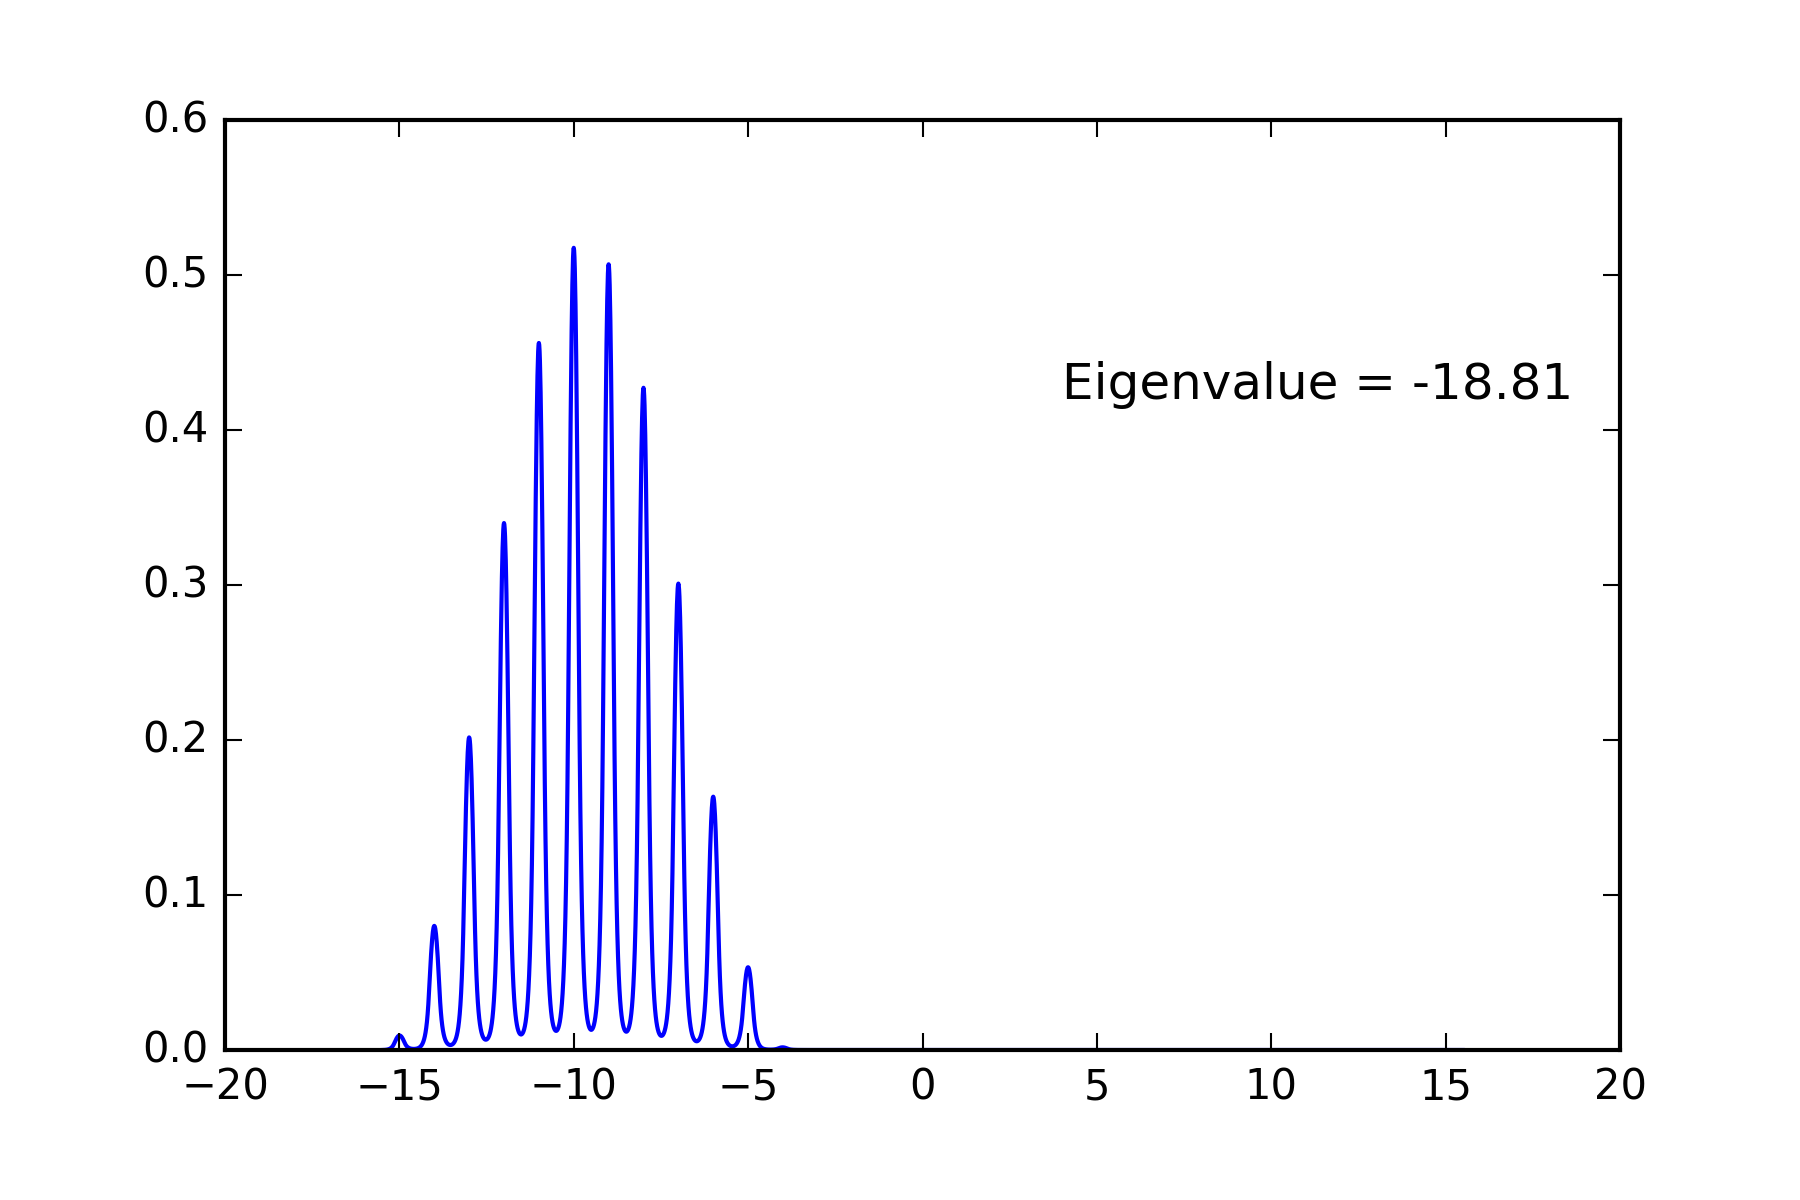
\includegraphics[width=1.1\linewidth]{floatingPrecision/oldPot100discrete_1th_Lowest0_3.png}
  \captionof{figure}{Old potential, $V_0l =10.0$, $l=0.4 $, discretization accuracy $= 0.01 $}
  \label{fig:oldPo_0.4}
\end{minipage}\qquad
\begin{minipage}{.45\textwidth}
  \centering
  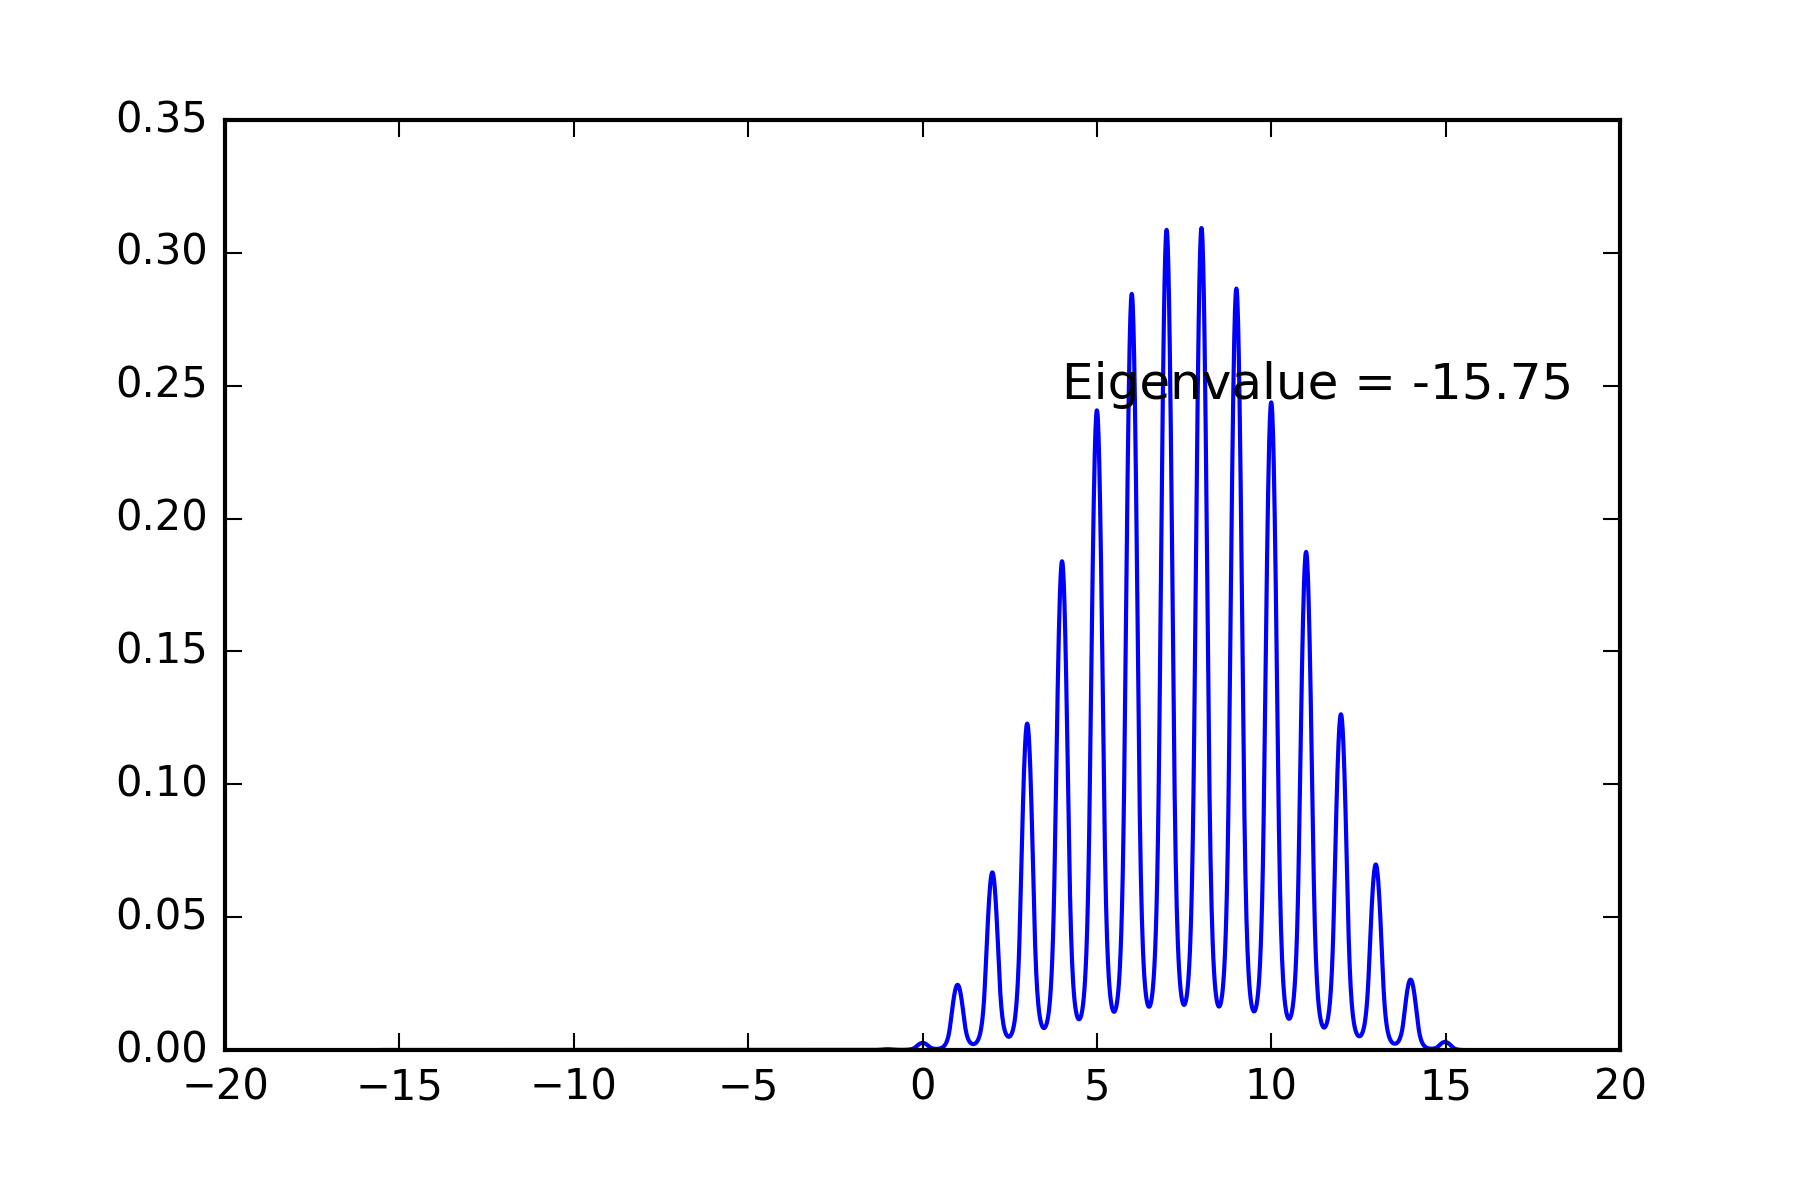
\includegraphics[width=1.1\linewidth]{floatingPrecision/oldPot100discrete_1th_Lowest0_4.png}
  \captionof{figure}{Old potential, $V_0l=10.0$, $l = 0.3 $,discretization accuracy $= 0.01$}
  \label{fig:oldPo_0.3}
\end{minipage}
\end{figure}

%old 
\begin{figure}[!htbh]
\centering
\begin{minipage}{.45\textwidth}
  \centering
  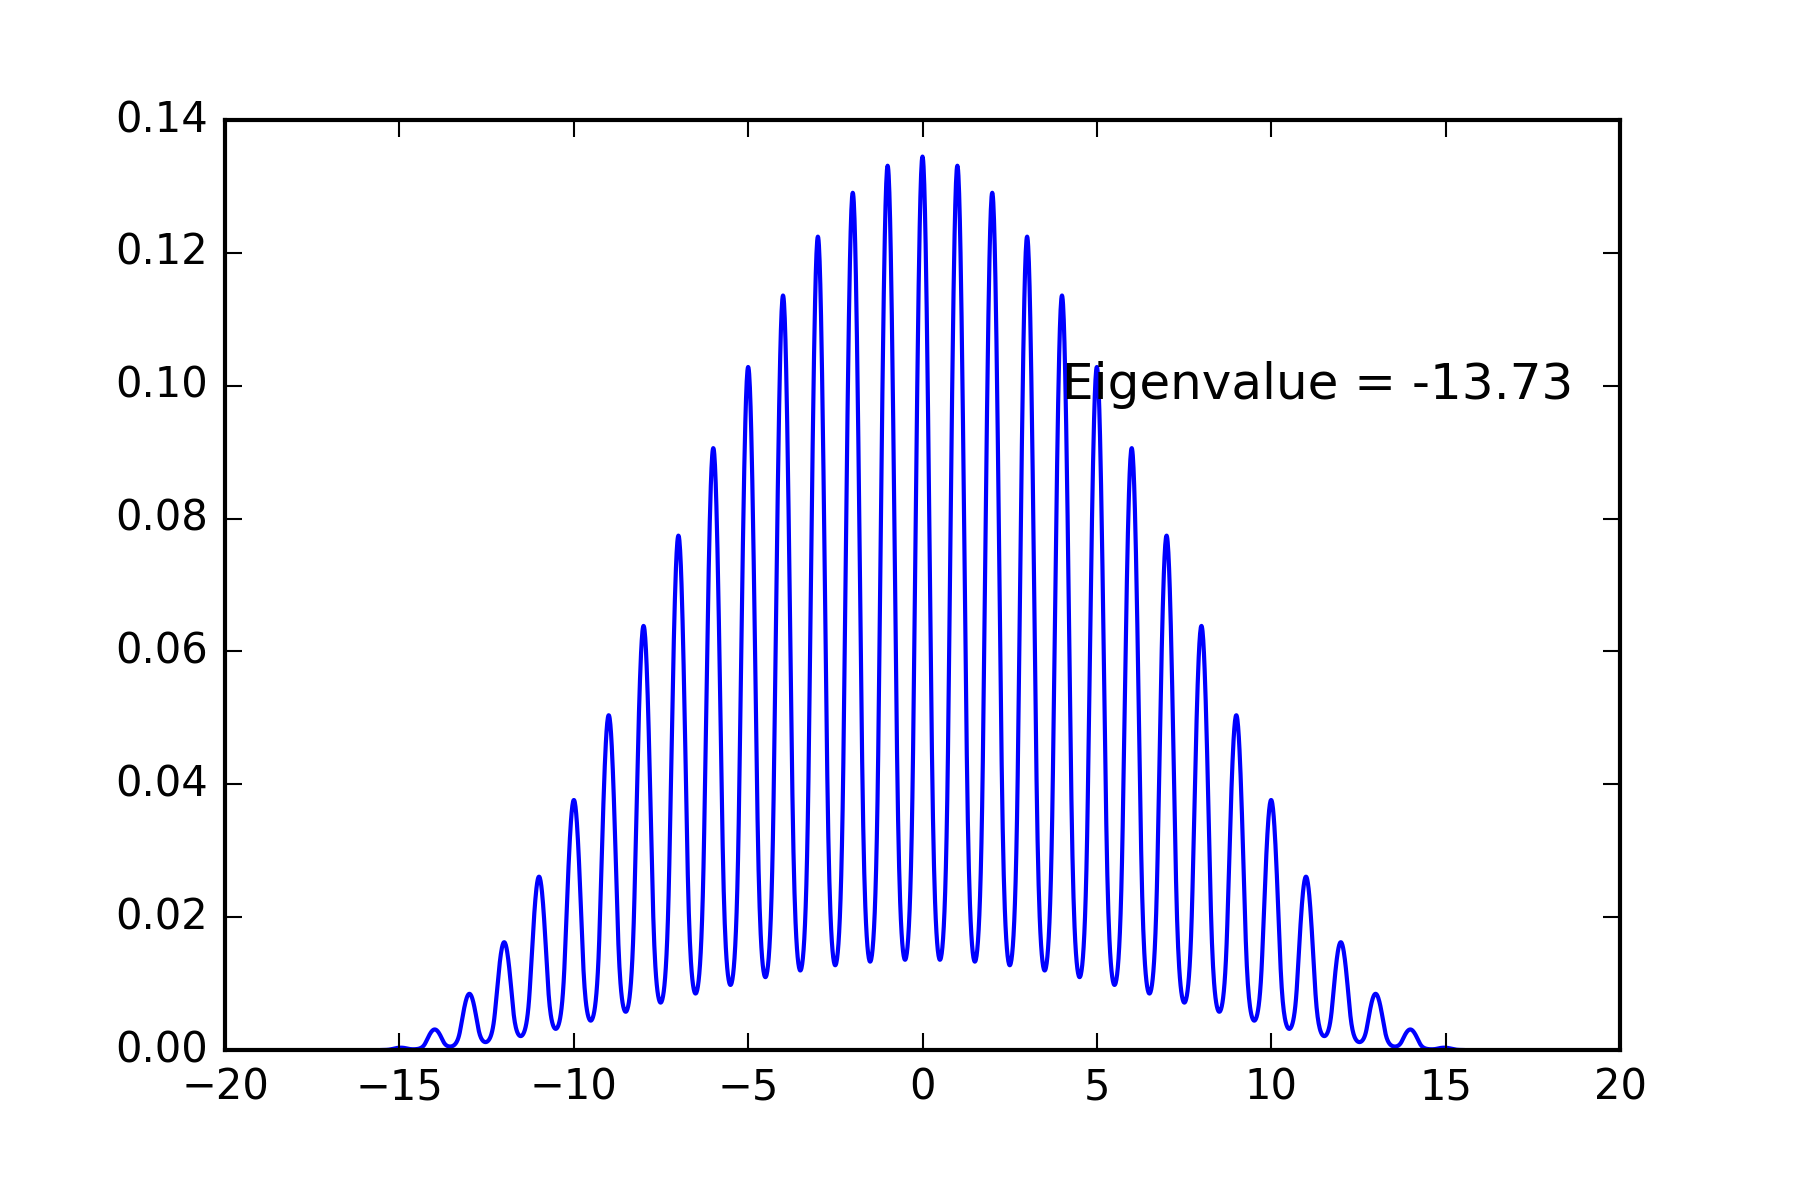
\includegraphics[width=1.1\linewidth]{floatingPrecision/oldPot100discrete_1th_Lowest0_5.png}
  \captionof{figure}{Old potential, $V_0l=10.0$, $l = 0.5 $,discretization accuracy $= 0.01 $}
  \label{fig:oldPo_0.5}
\end{minipage}\qquad
%new
\begin{minipage}{.45\textwidth}
  \centering
  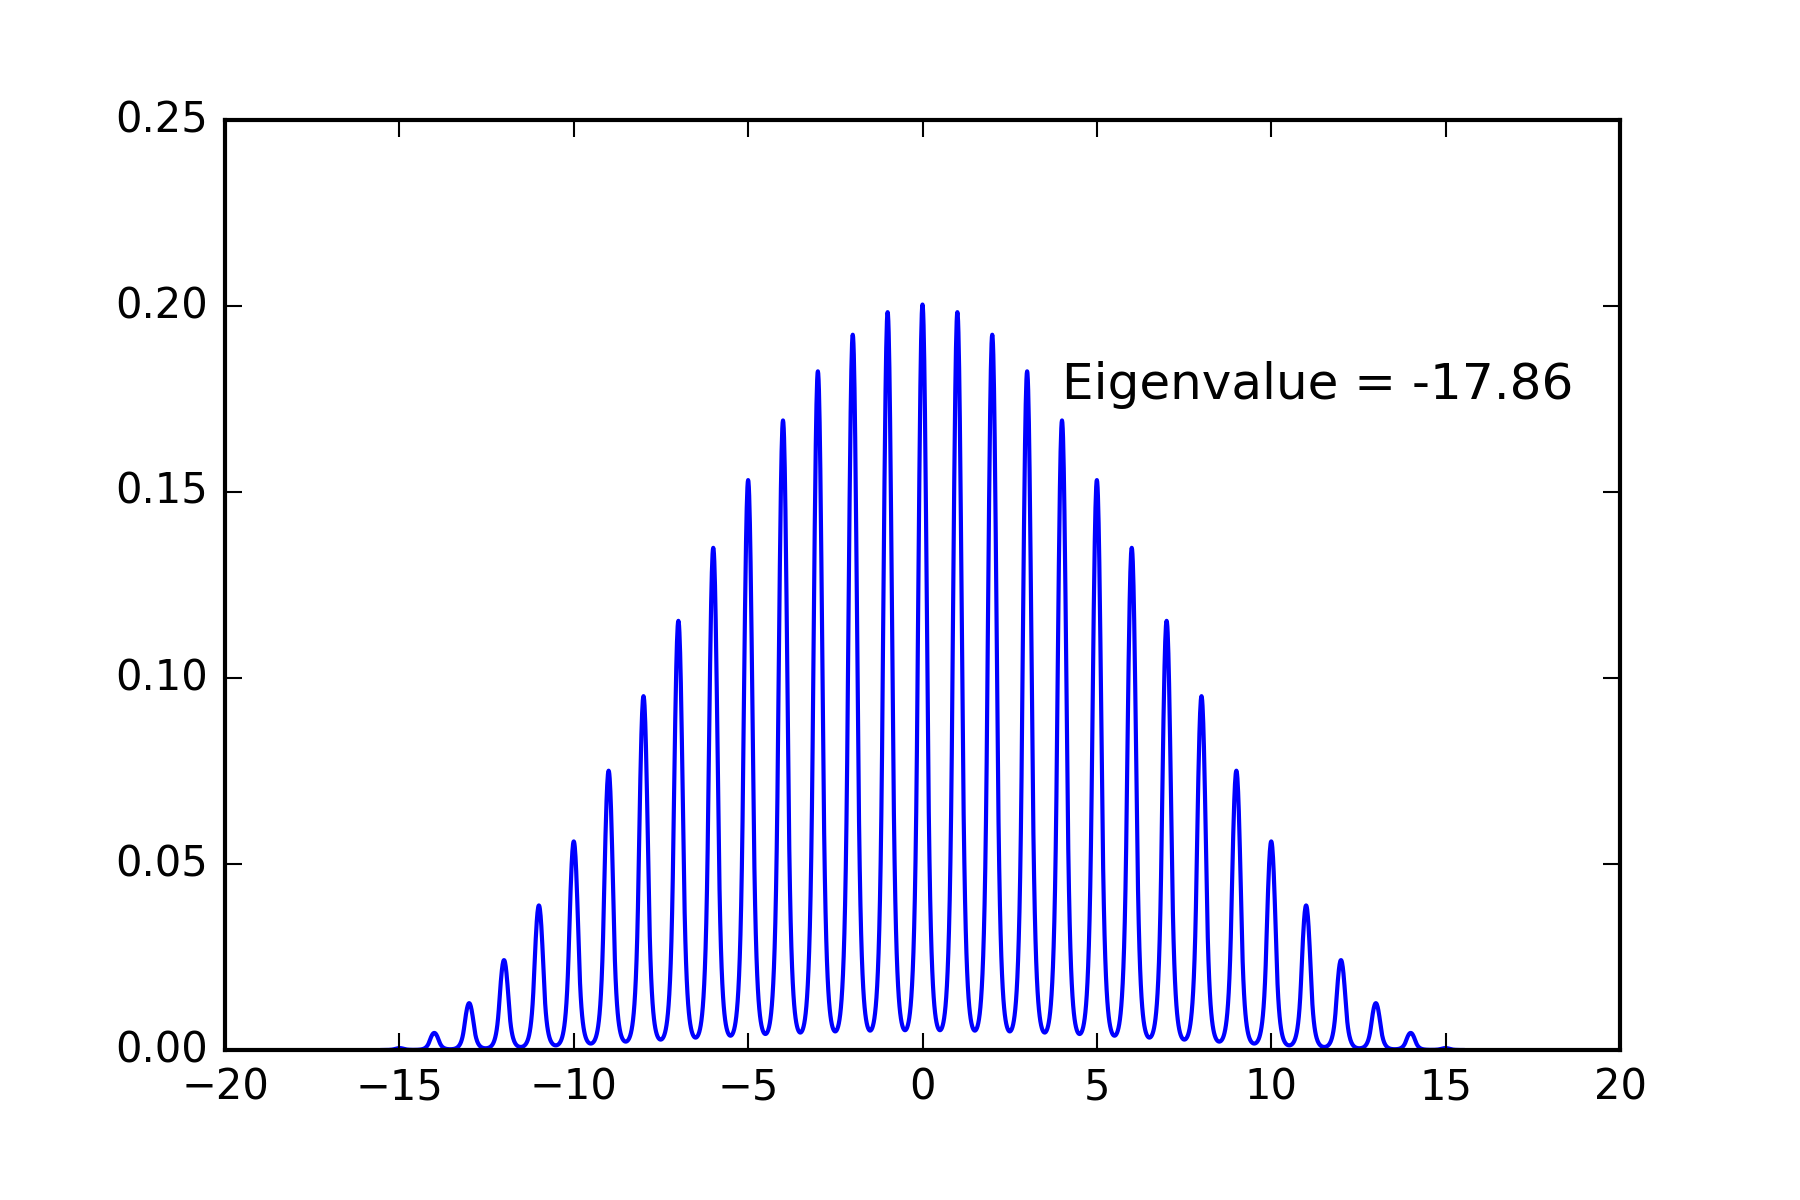
\includegraphics[width=1.1\linewidth]{floatingPrecision/newPot100discrete_1th_Lowest0_3.png}
  \captionof{figure}{New potential,  $V_0l=10.0$, $l = 0.3 $,discretization accuracy $= 0.01 $}
  \label{fig:newPo_0.3}
\end{minipage}
\end{figure}

%new
\begin{figure}[!htbh]
\centering
\begin{minipage}{.45\textwidth}
  \centering
  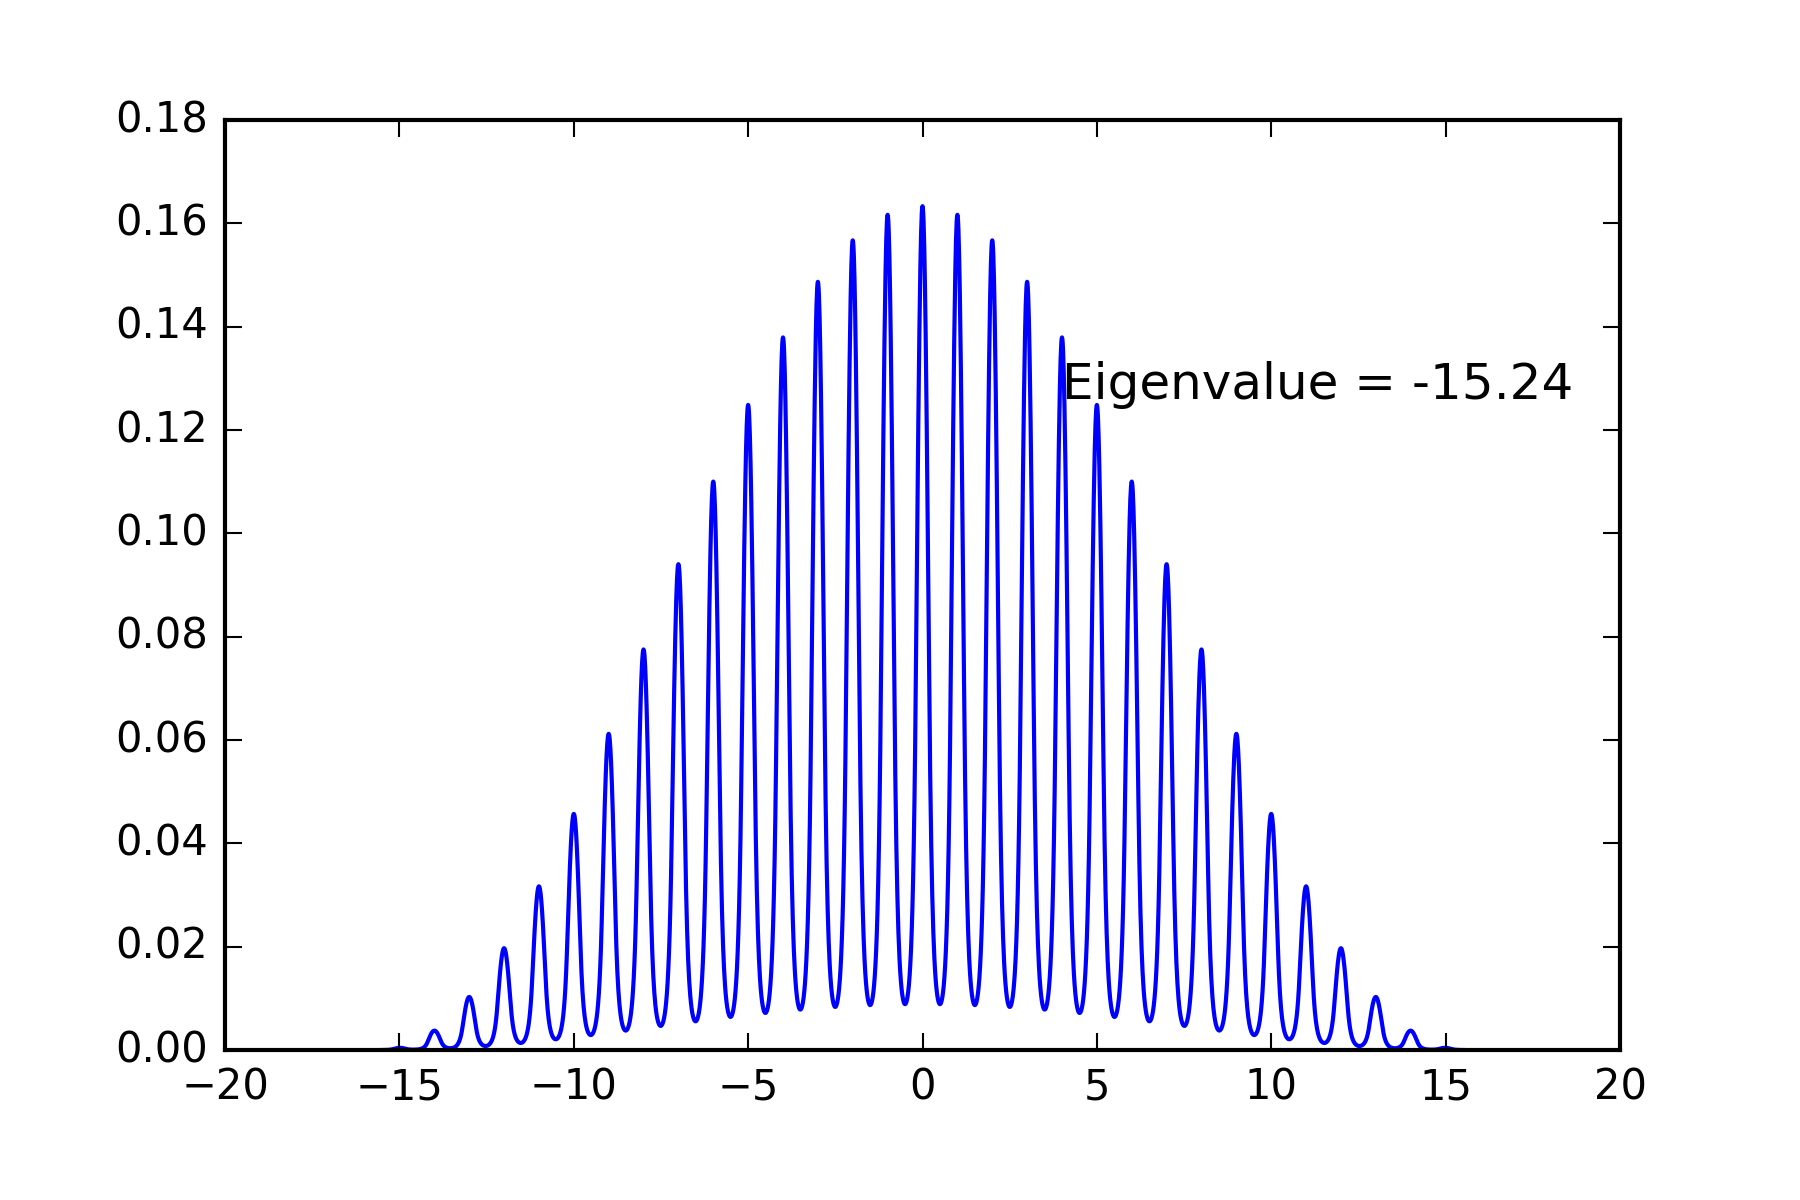
\includegraphics[width=1.1\linewidth]{floatingPrecision/newPot100discrete_1th_Lowest0_4.png}
  \captionof{figure}{New potential,  $V_0l=10.0$, $l = 0.4 $, discretization accuracy $= 0.01 $}
  \label{fig:newPo_0.4}
\end{minipage}\qquad
\begin{minipage}{.45\textwidth}
  \centering
  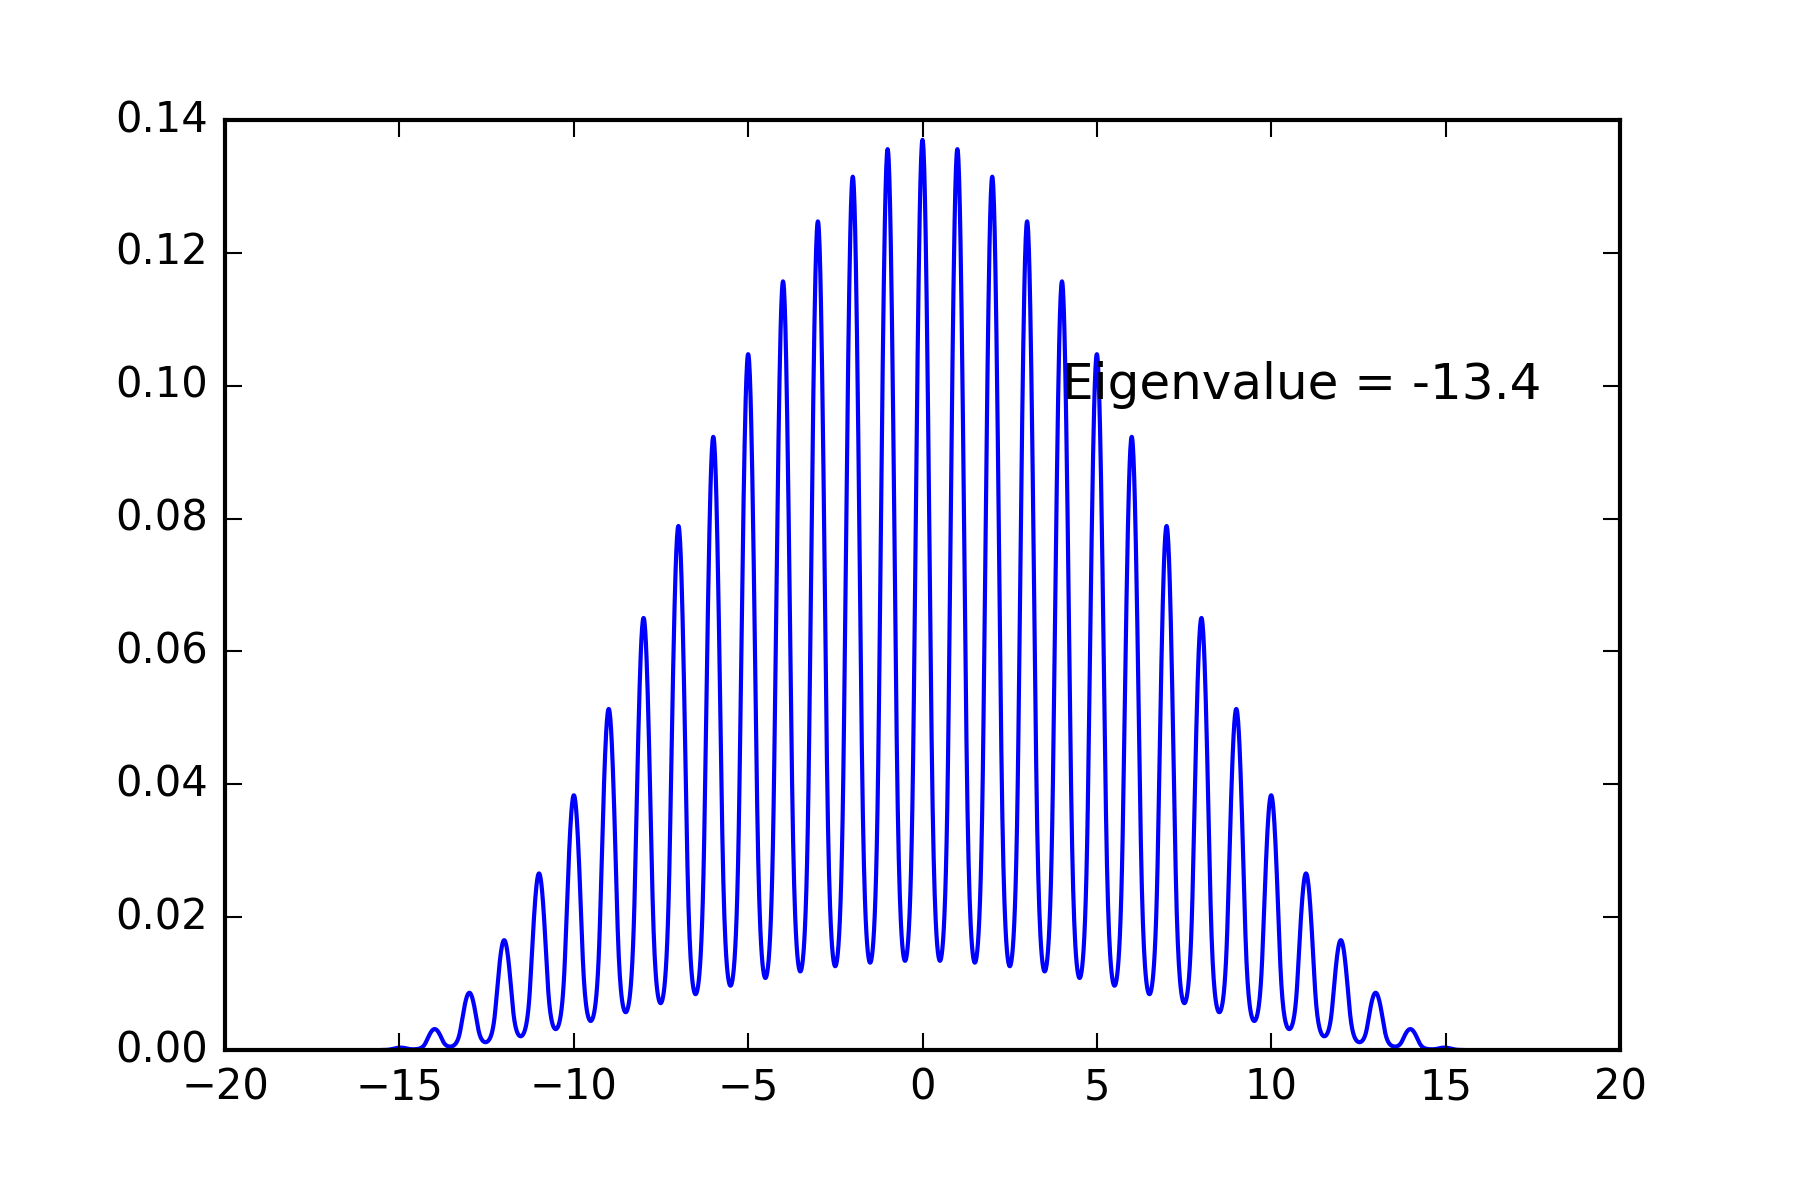
\includegraphics[width=1.1\linewidth]{floatingPrecision/newPot100discrete_1th_Lowest0_5.png}
  \captionof{figure}{New potential, $V_0l=10.0$, $l = 0.5 $, discretization accuracy $= 0.01 $}
  \label{fig:newPo_0.5}
\end{minipage}
\end{figure}

%A measure for degree of localization
\newpage
\subsection{A measure for degree of localization}
We try a way of defining degree of localization for eigenstates using standard deviation, which can be computed from the probability density function.
The advantage of defining such a measure is to allow us to compare localization quantitatively under different conditions. With this measure, we can also plot the standard deviations at different energy levels for two systems, namely a regular system, and a disordered system, in order to compare localization at different energy levels. 
Note that for the disordered system, we handle randomness by computing the standard deviations for 101 samples and taking an average.

The parameters for the regular and disordered systems are listed below in the table (Note that each parameter is defined in previous sections) followed by the corresponding figures for standard deviations against energy levels. 


\newpage
\begin{table}[]
\centering
\begin{tabular}{|l|l|l|l|l|}
\hline
	 & number of atoms  &$V_0l$& atomic spacings & probabilities   \\ \hline
Regular system&31& 10.0  & {1.0}  & {1} \\ \hline
Disordered System No.1 &31 &10.0   & {1.1,1.0}  & {0.5,0.5}    \\ \hline
Disordered System No.2 &31 &10.0   & {1.5,1.0}  & {0.5,0.5}    \\ \hline
Disordered System No.3 &31 &30.0   & {1.1,1.0}  & {0.5,0.5}    \\ \hline
Disordered System No.4 &31 &30.0   & {1.1,1.0}  & {0.5,0.5}    \\ \hline
\end{tabular}
\centering
\end{table}



%start figure
\begin{figure}[!htbh]
\centering
\begin{minipage}{.45\textwidth}
  \centering
  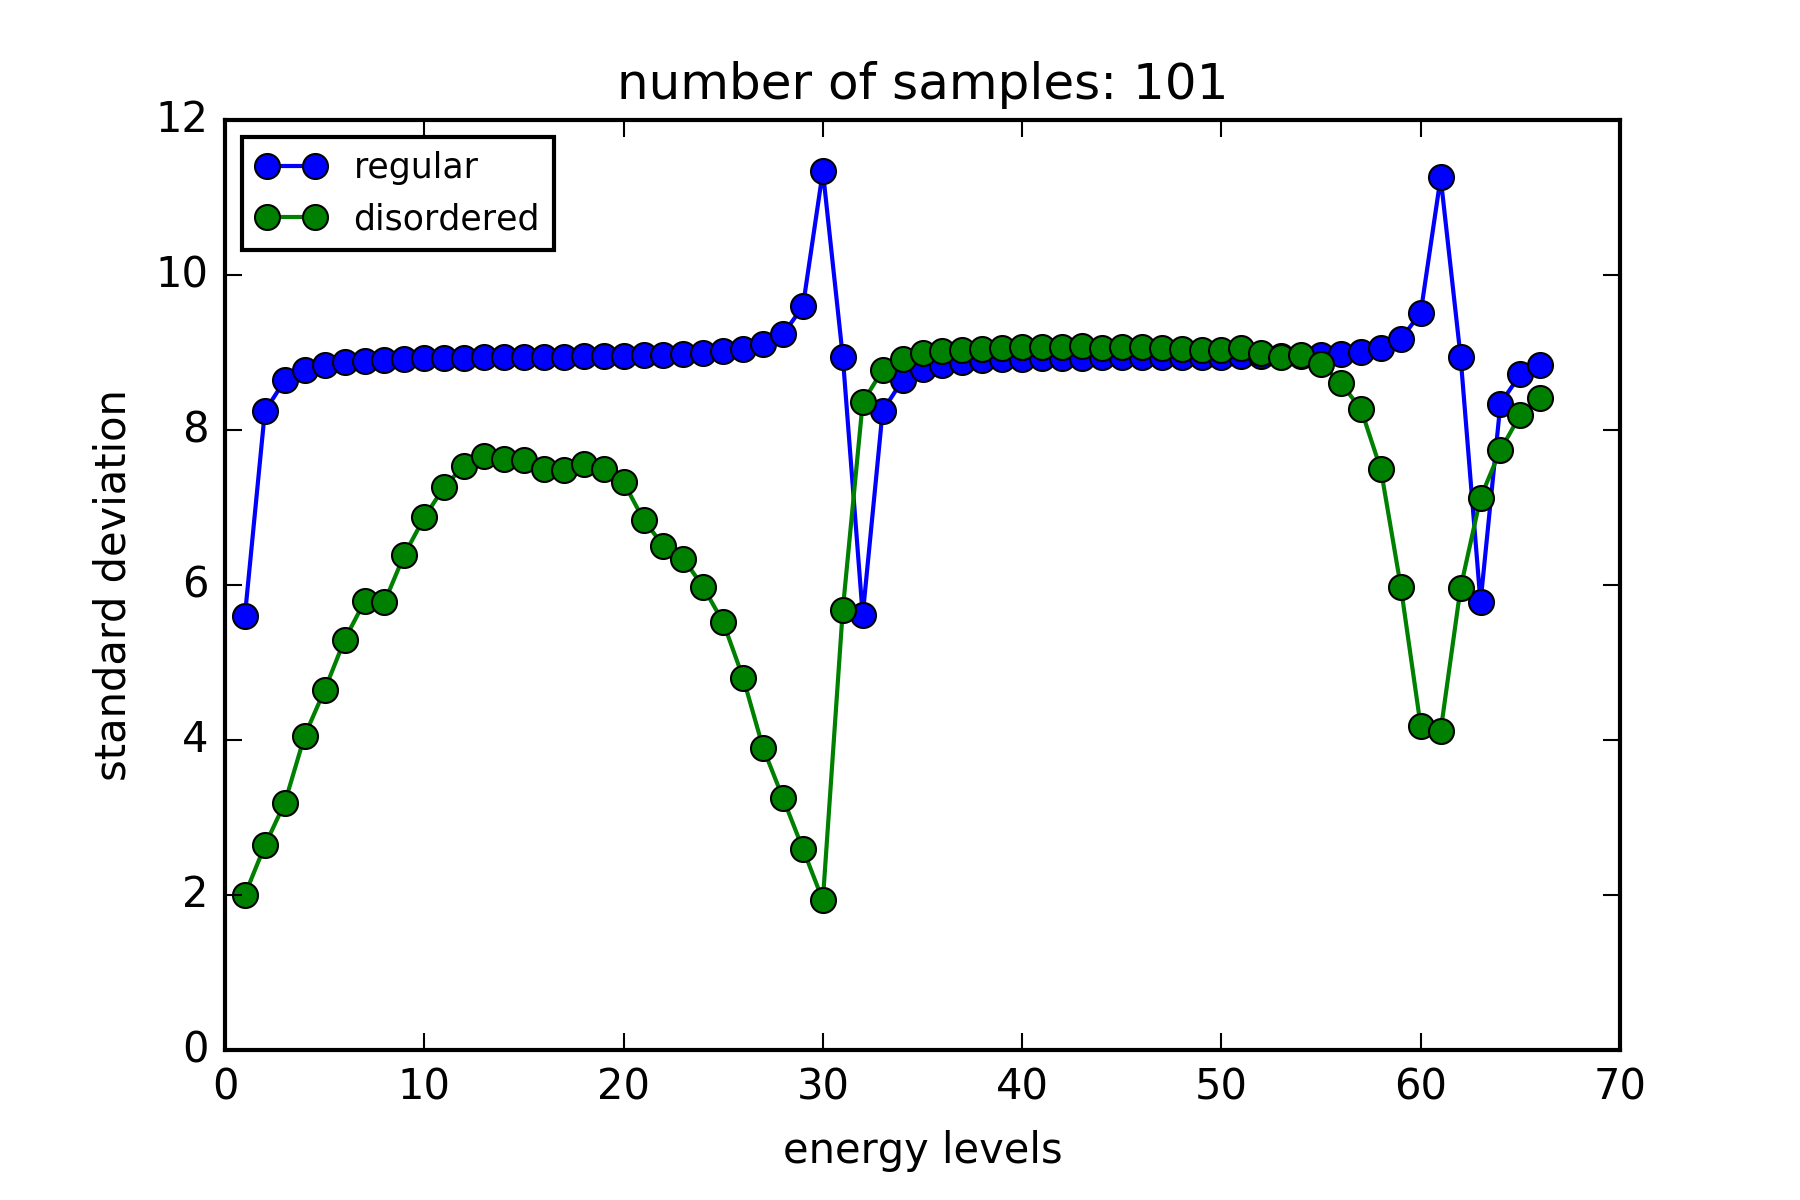
\includegraphics[width=1.1\linewidth]{standardDeviation/N_31_100a10_0_1_1_p_0_5.png}
  \captionof{figure}{Localization against energy levels, comparison between Regular System and Disordered System No.1}
  \label{fig:disordered sys num 1}
\end{minipage}\qquad
\begin{minipage}{.45\textwidth}
  \centering
  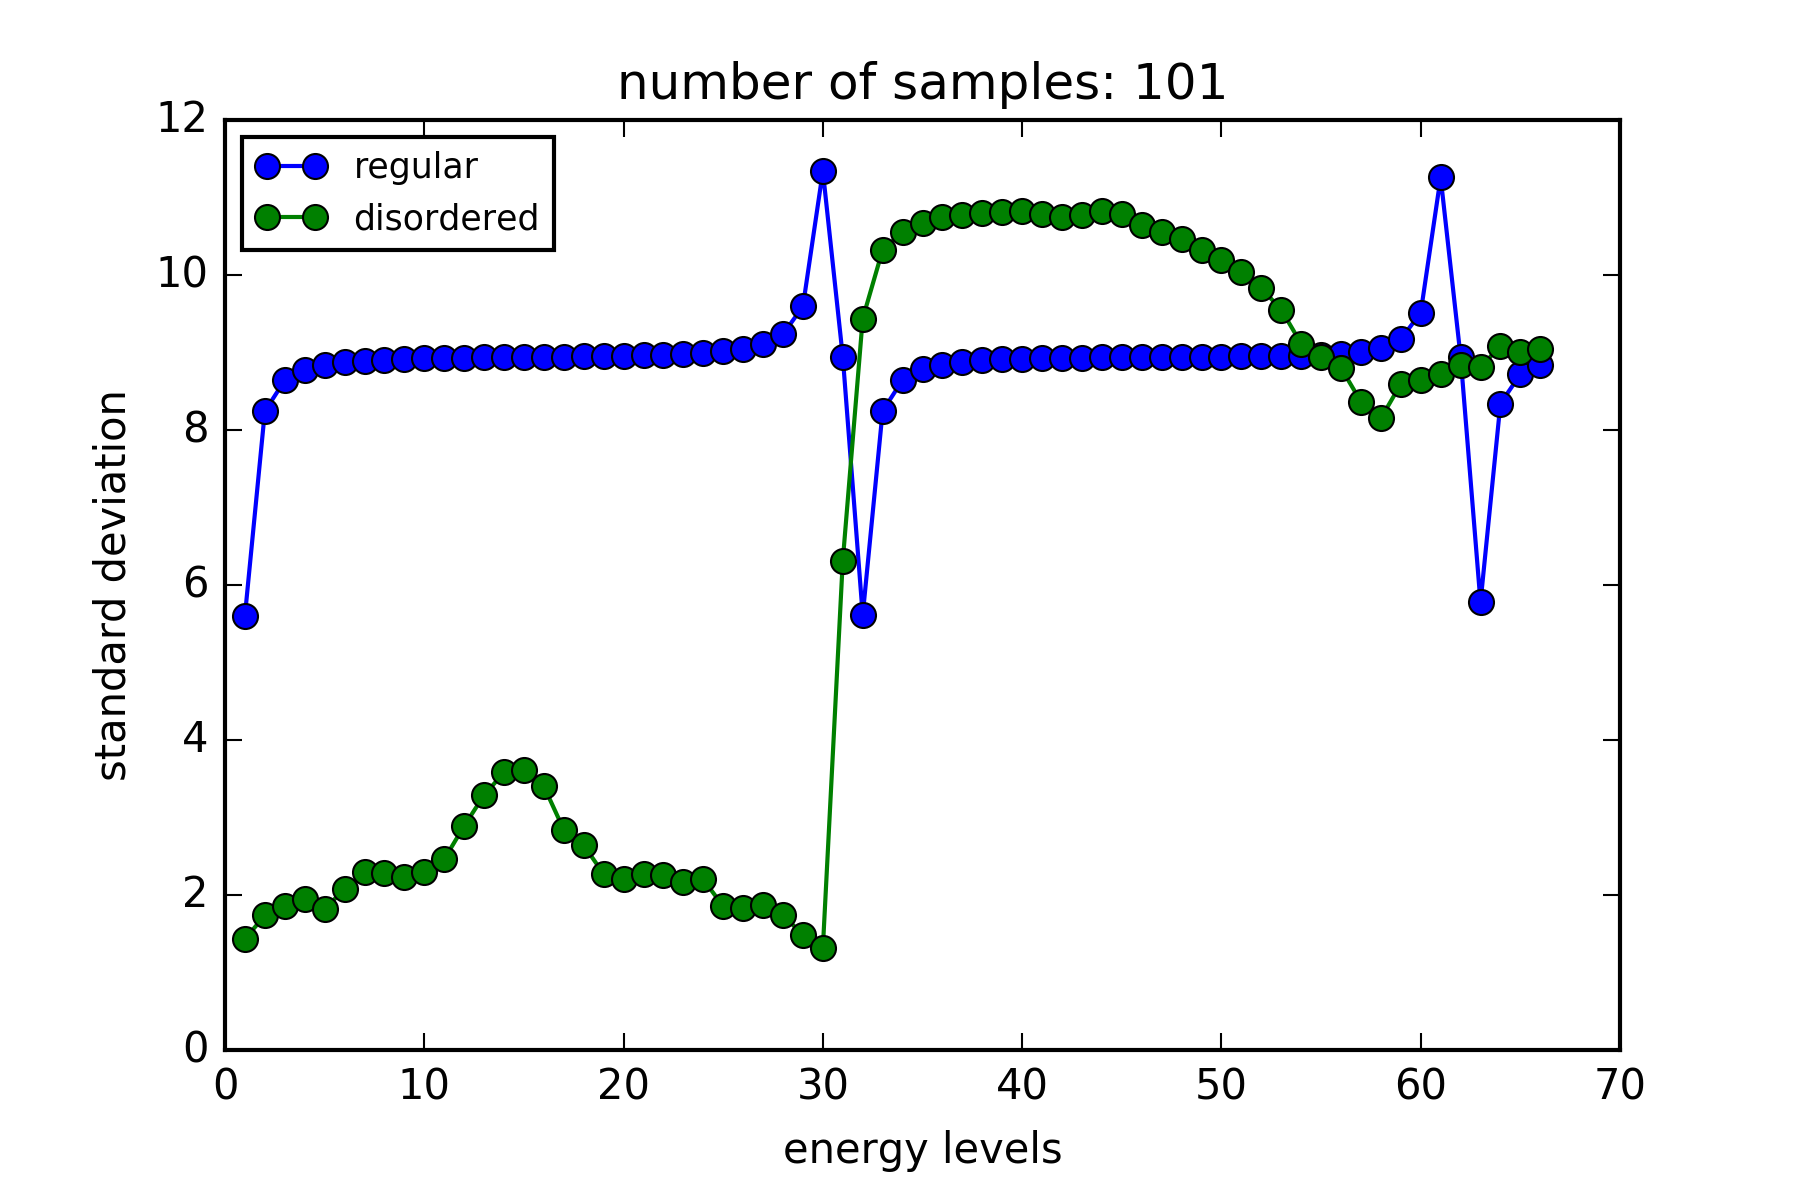
\includegraphics[width=1.1\linewidth]{standardDeviation/N_31_100a10_0_1_5_p_0_5.png}
  \captionof{figure}{Localization against energy levels, comparison between Regular System and Disordered System No.2}
  \label{fig:disordered sys num 2}
\end{minipage}
\end{figure}

%a = 30 
\begin{figure}[!htbh]
\centering
\begin{minipage}{.45\textwidth}
  \centering
  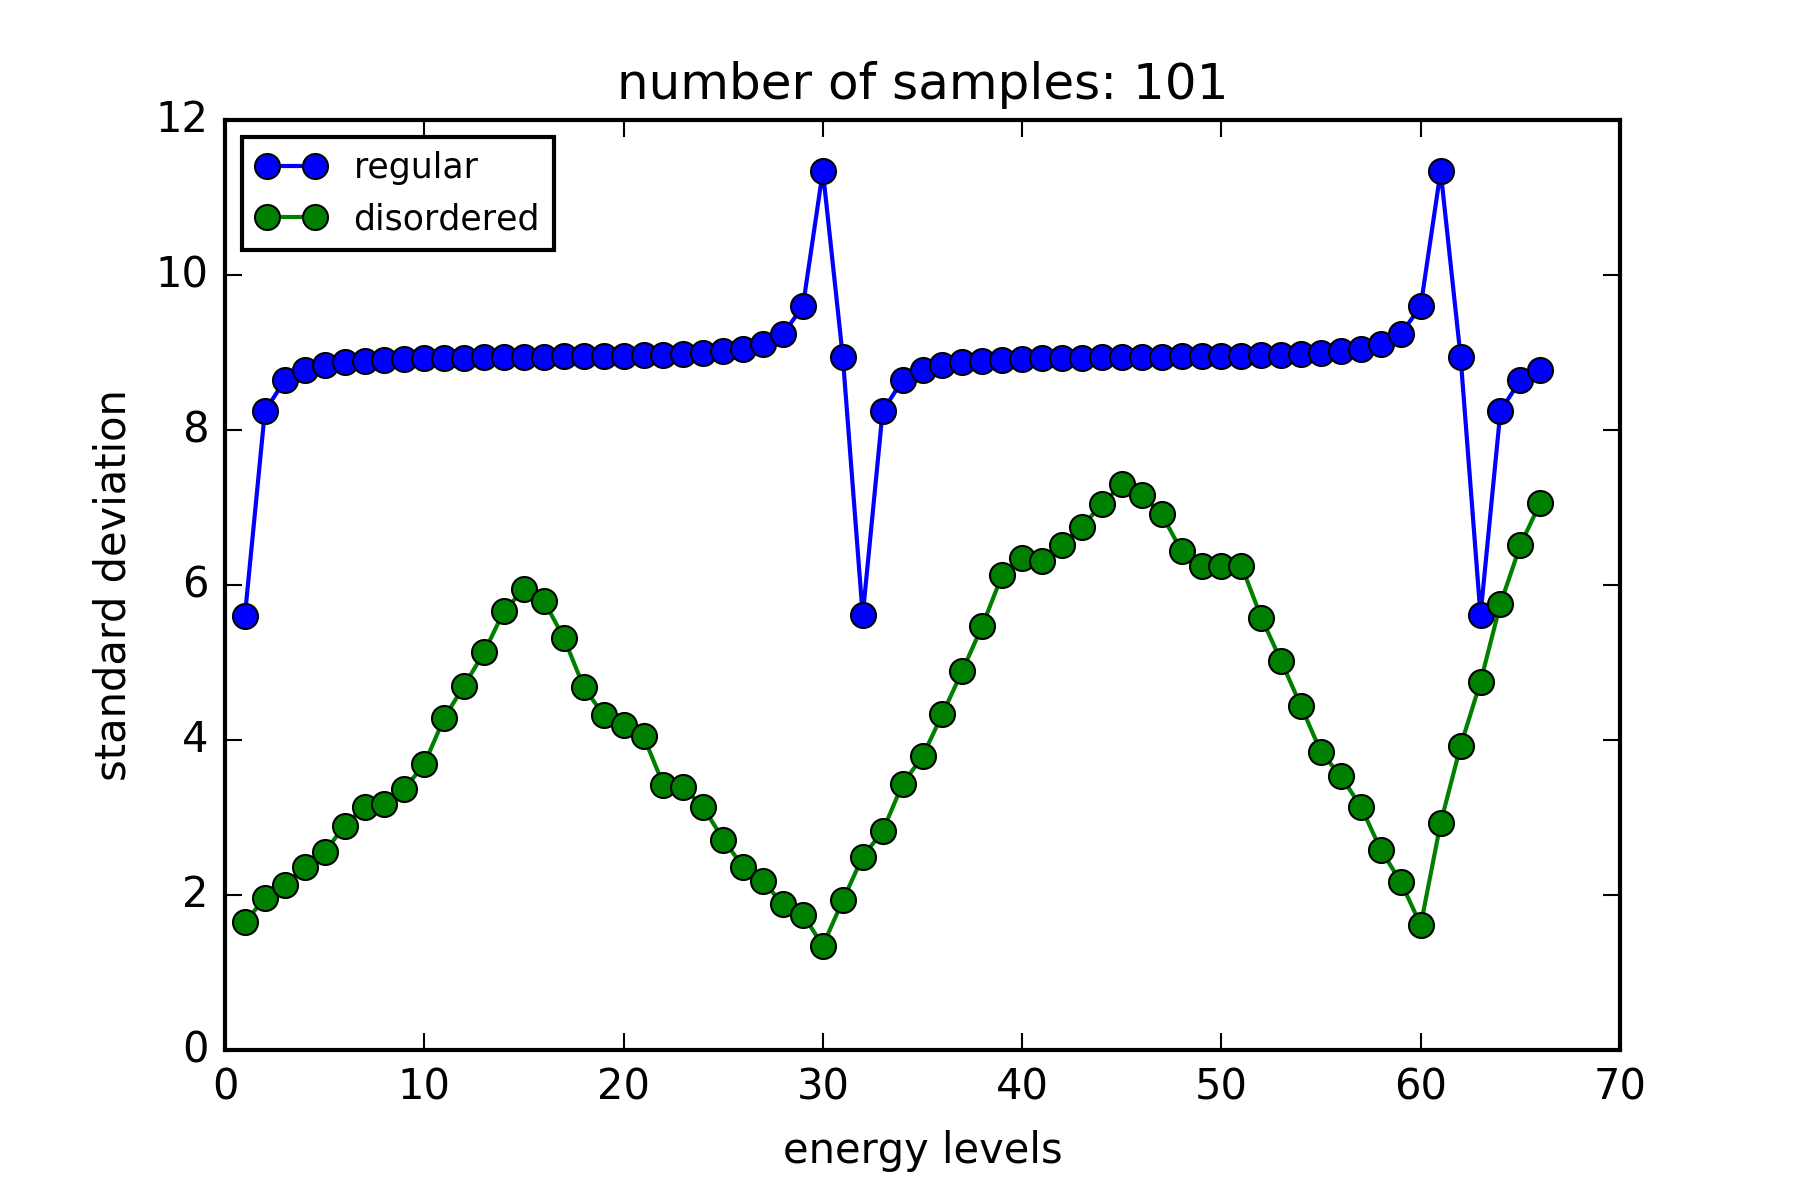
\includegraphics[width=1.1\linewidth]{standardDeviation/N_31_100a30_0_1_1_p_0_5.png}
  \captionof{figure}{Localization against energy levels, comparison between Regular System and Disordered System No.3}
  \label{fig:disordered sys num 3}
\end{minipage}\qquad
\begin{minipage}{.45\textwidth}
  \centering
  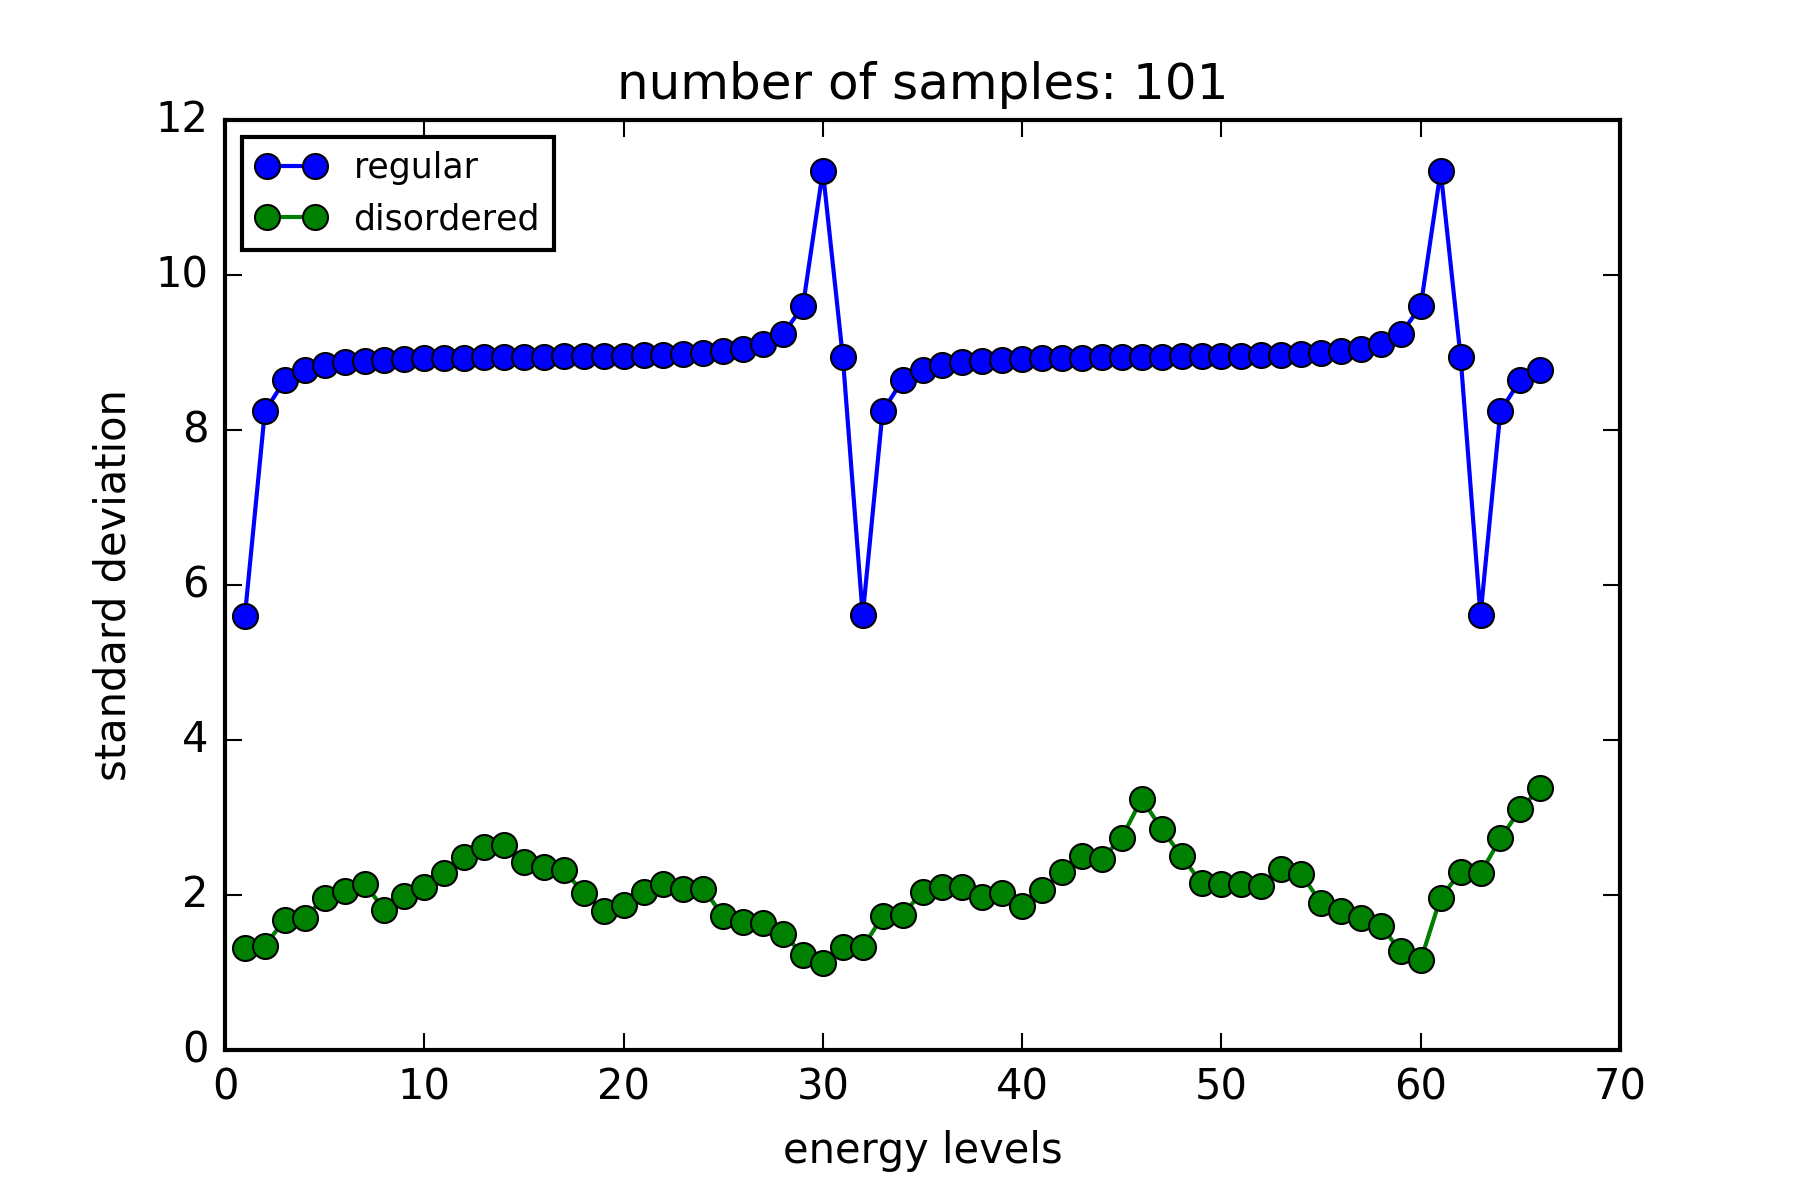
\includegraphics[width=1.1\linewidth]{standardDeviation/N_31_100a30_0_1_5_p_0_5.png}
  \captionof{figure}{Localization against energy levels, comparison between Regular System and Disordered System No.4}
  \label{fig:disordered sys num 4}
\end{minipage}
\end{figure}
%end figure

The following are figures for disordered systems with randomness in potential, in which we fix the square potential area and pick the well width from two values$\{w_1,w_2\}$ with probability $\{0.5,0.5\}$. 
The table lists the parameters for the regular system and different disordered systems. 

\newpage
\begin{table}[]
\centering
\begin{tabular}{|l|l|l|l|l|}
\hline
	 & number of atoms  &$V_0l$& well width $\{w_1,w_2\}$ & probabilities   \\ \hline
Regular system&31& 10.0  & {0.5}  & {1} \\ \hline
Disordered System No.5 &31 &10.0   & {0.4,0.5}  & {0.5,0.5}    \\ \hline
Disordered System No.6 &31 &10.0   & {0.2,0.5}  & {0.5,0.5}    \\ \hline
Disordered System No.7 &31 &30.0   & {0.4,0.5}  & {0.5,0.5}    \\ \hline
Disordered System No.8 &31 &30.0   & {0.2,0.5}  & {0.5,0.5}    \\ \hline
\end{tabular}
\centering
\end{table}

%randomness in potential 

%start figure
\begin{figure}[!htbh]
\centering
\begin{minipage}{.45\textwidth}
  \centering
  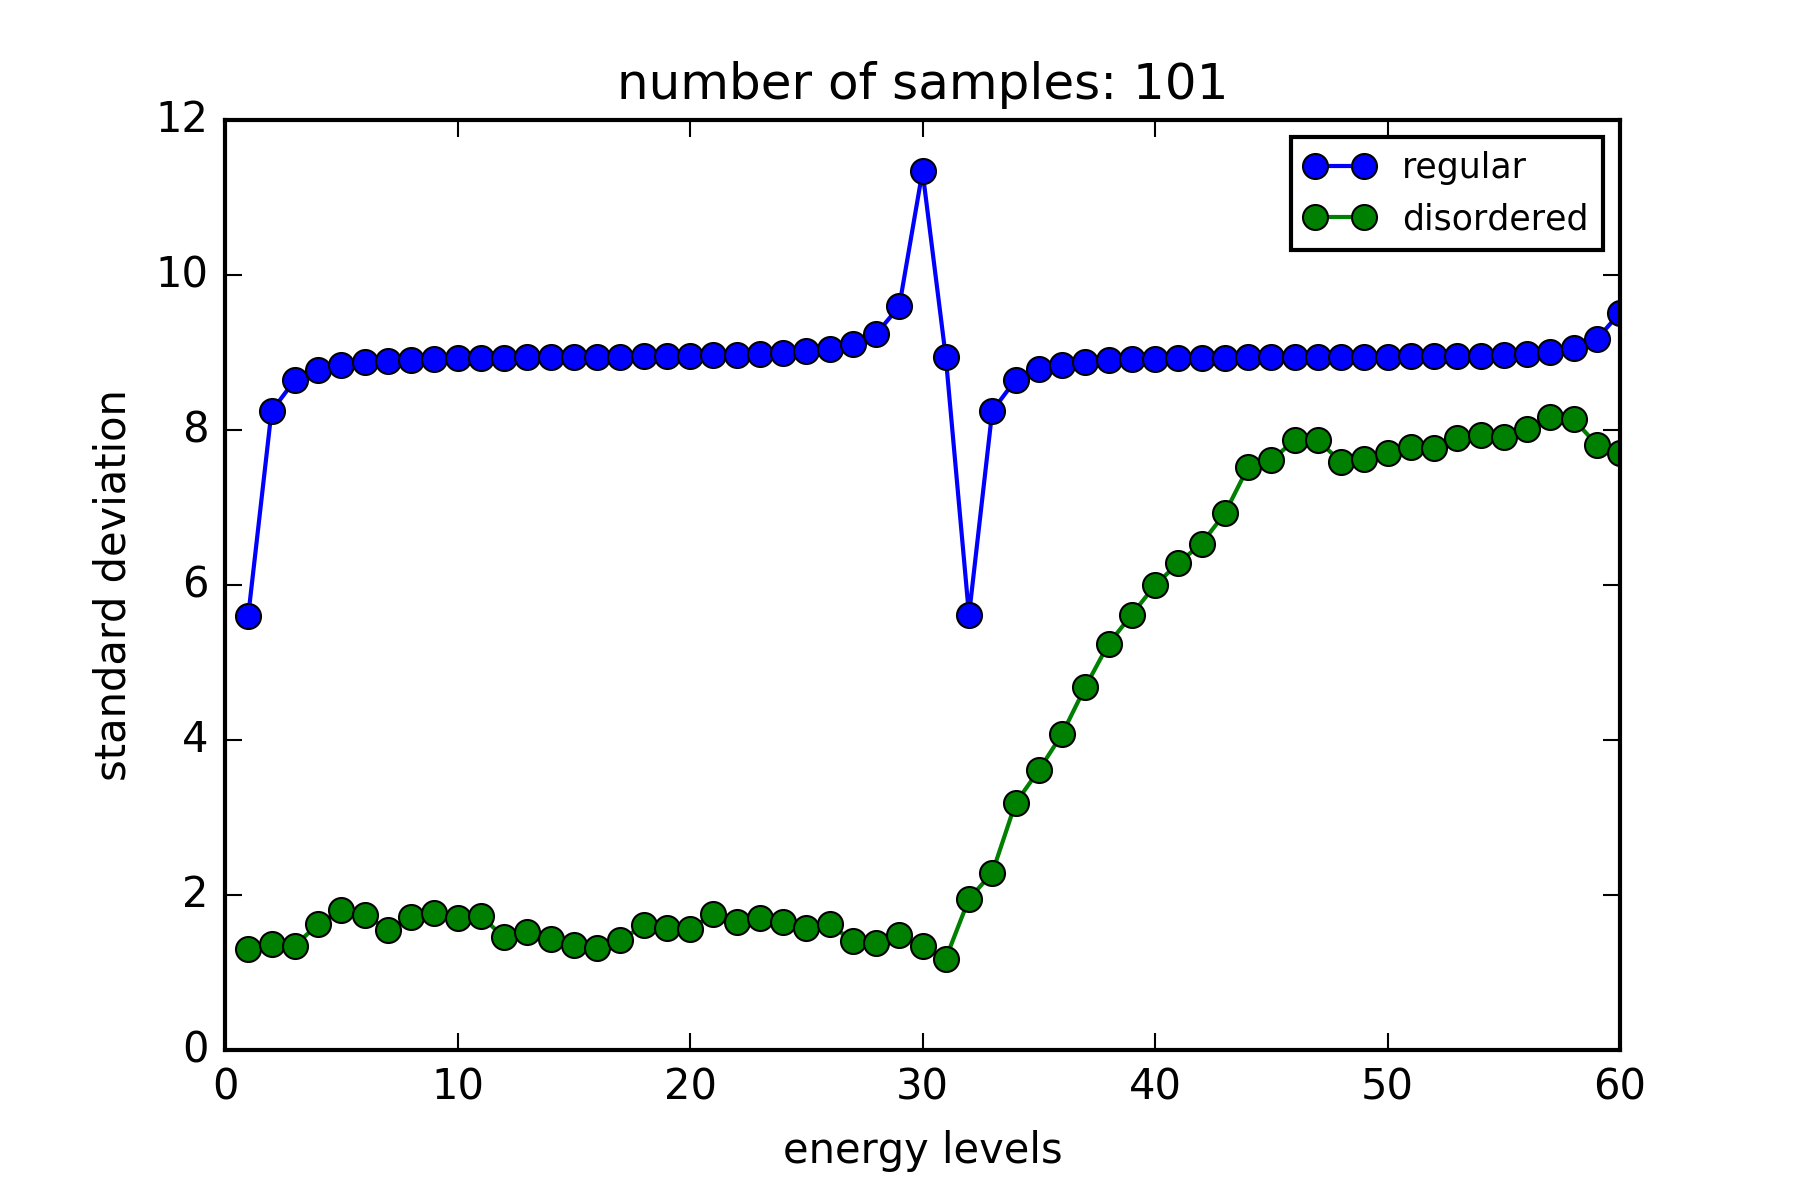
\includegraphics[width=1.1\linewidth]{standardDeviation/N_31_100a10_well0_4_p_0_5.png}
  \captionof{figure}{Localization against energy levels, comparison between Regular System and Disordered System No.5}
  \label{fig:disordered sys num 5}
\end{minipage}\qquad
\begin{minipage}{.45\textwidth}
  \centering
  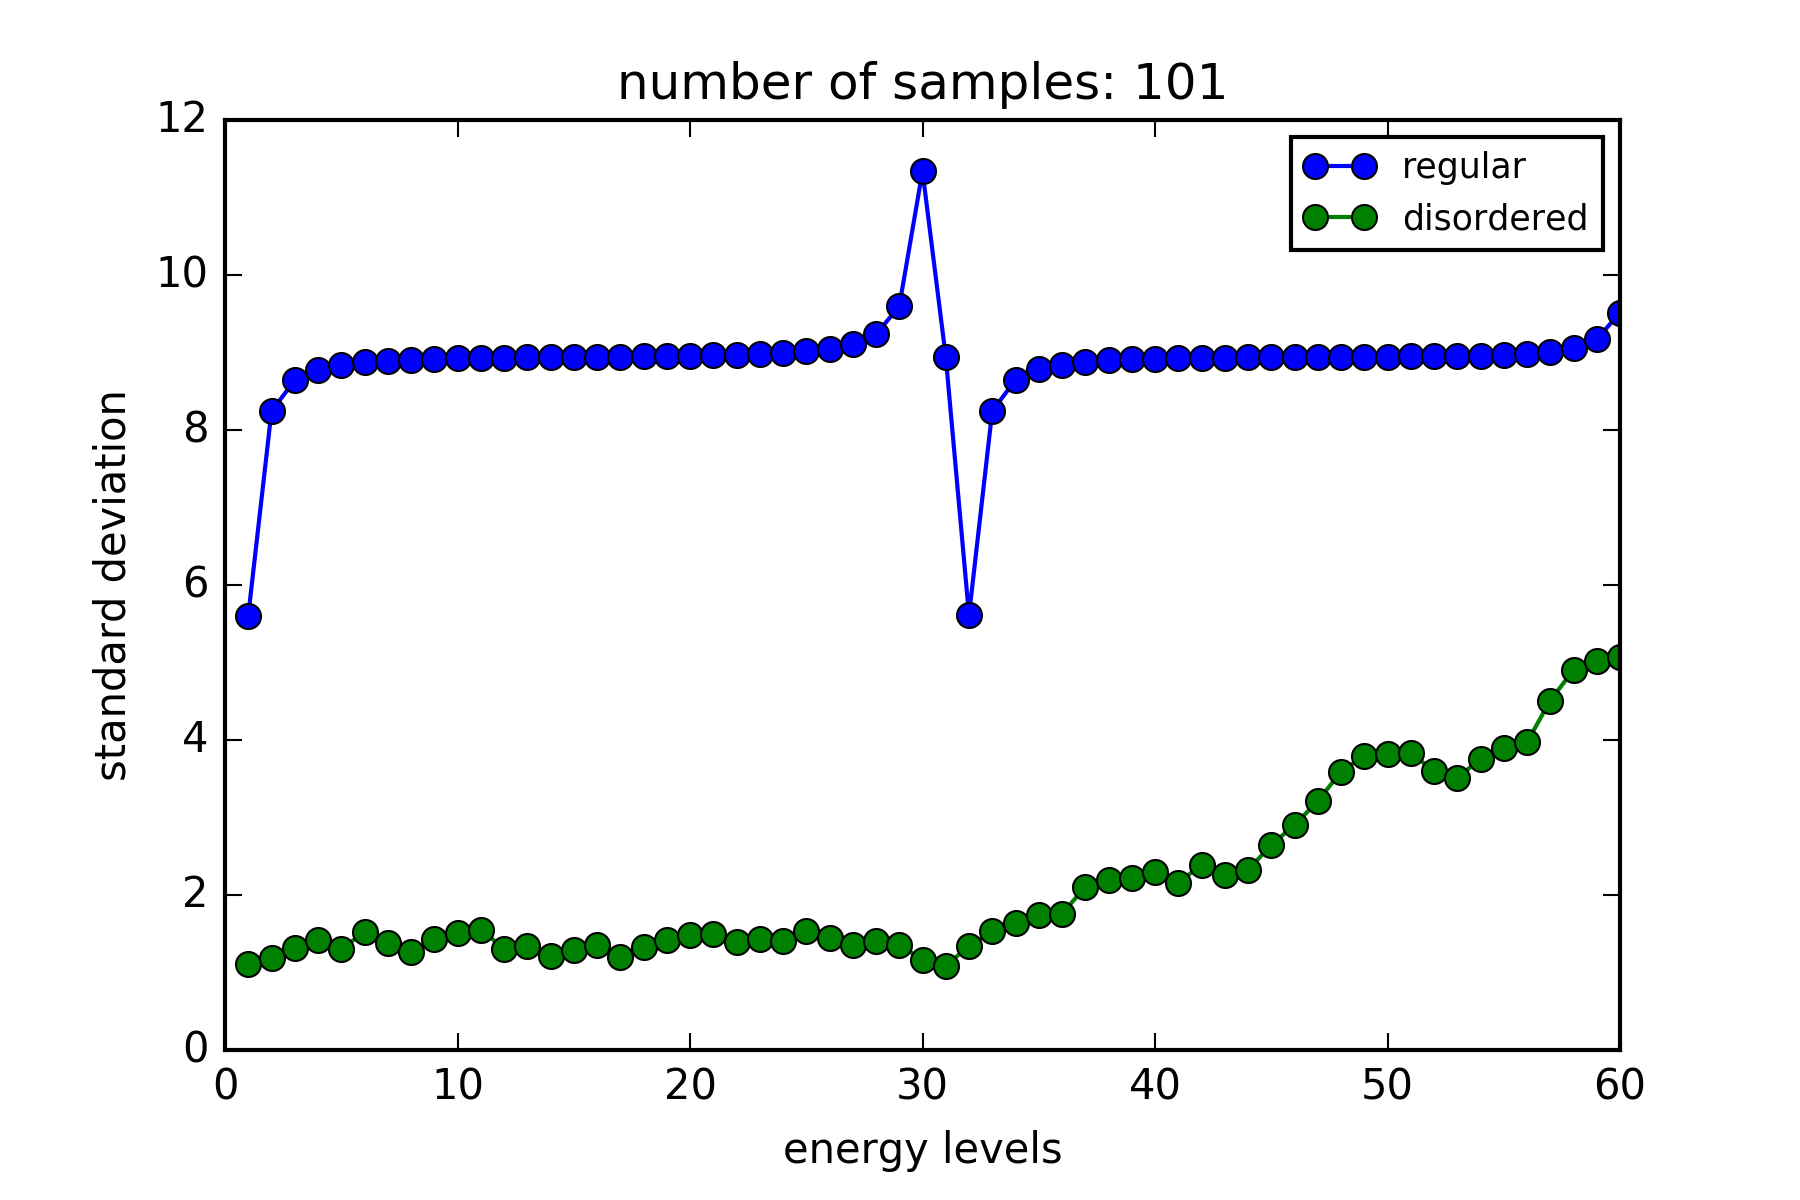
\includegraphics[width=1.1\linewidth]{standardDeviation/N_31_100a10_well0_2_p_0_5.png}
  \captionof{figure}{Localization against energy levels, comparison between Regular System and Disordered System No.6}
  \label{fig:disordered sys num 6}
\end{minipage}
\end{figure}

%a = 30 
\begin{figure}[!htbh]
\centering
\begin{minipage}{.45\textwidth}
  \centering
  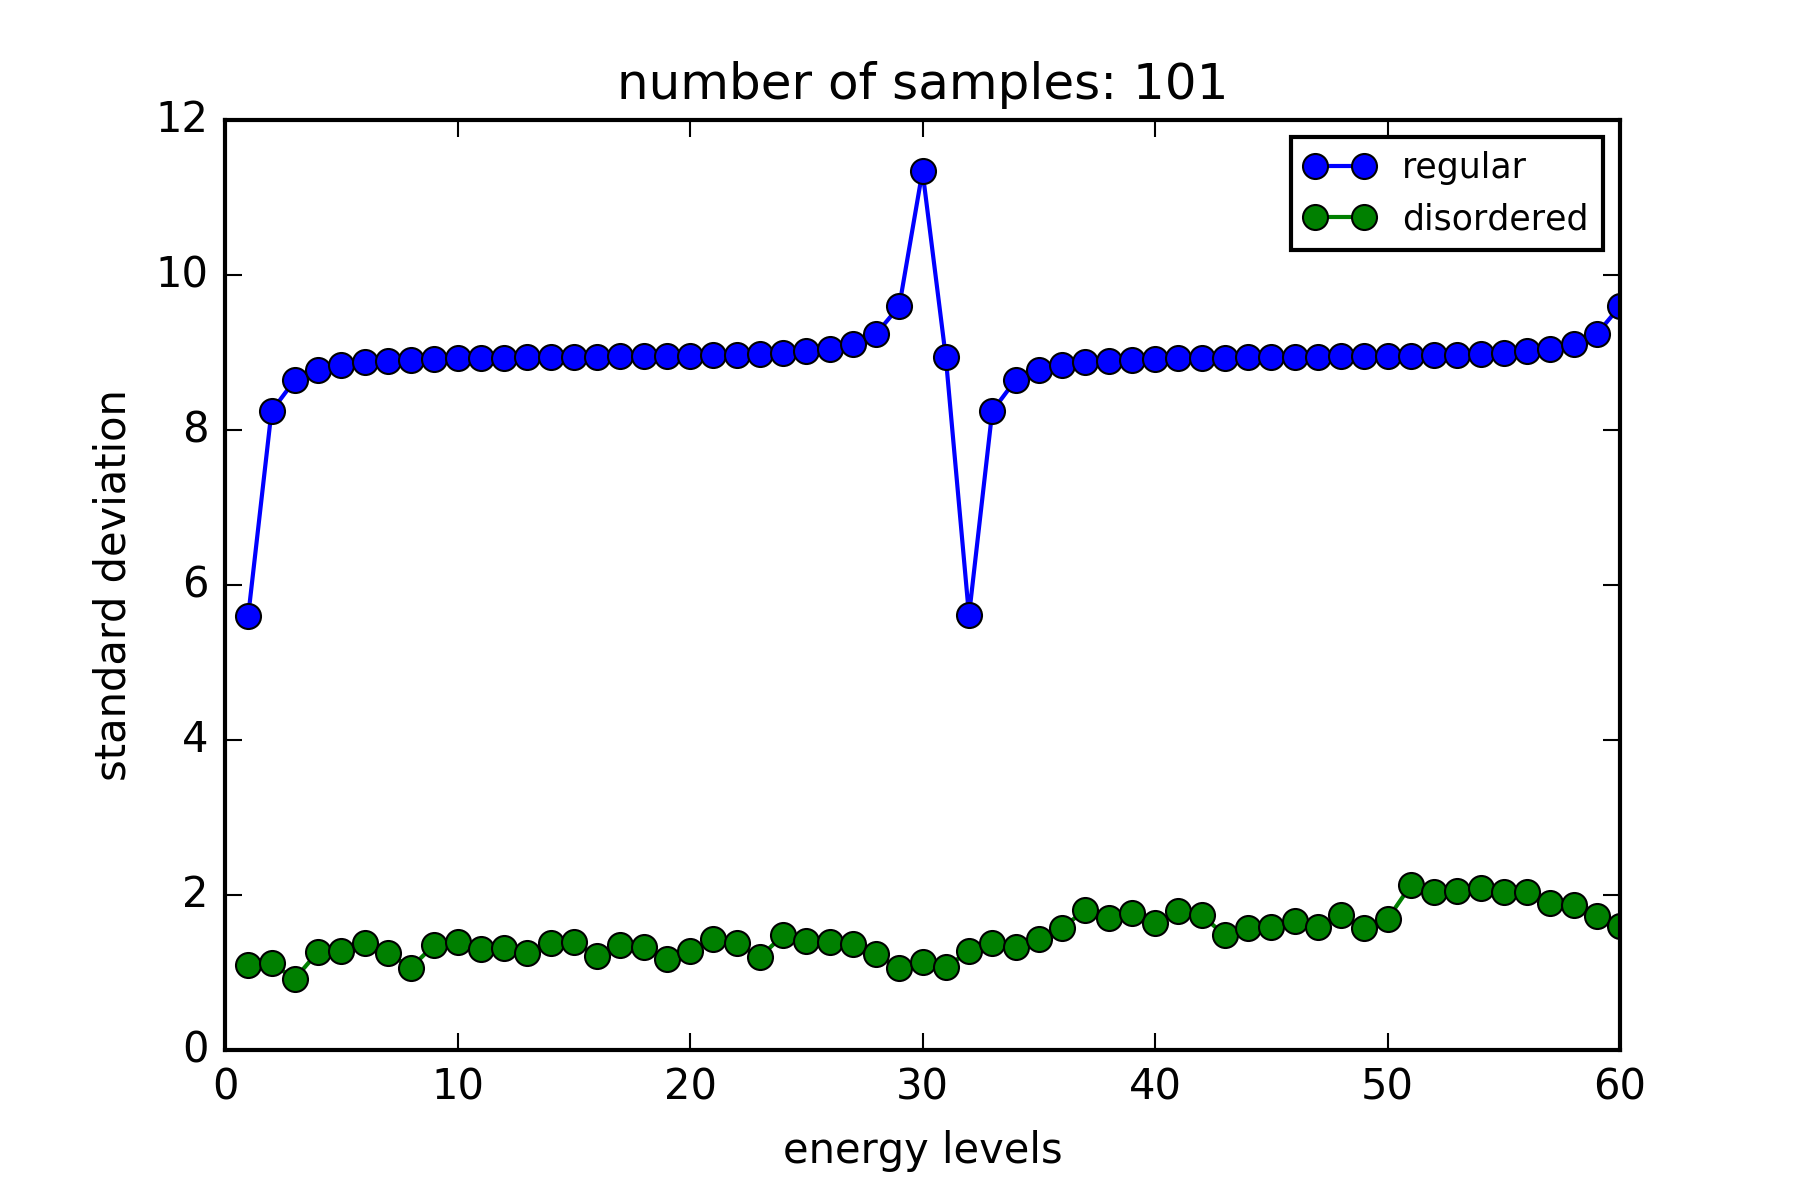
\includegraphics[width=1.1\linewidth]{standardDeviation/N_31_100a30_well0_4_p_0_5.png}
  \captionof{figure}{Localization against energy levels, comparison between Regular System and Disordered System No.7}
  \label{fig:disordered sys num 7}
\end{minipage}\qquad
\begin{minipage}{.45\textwidth}
  \centering
  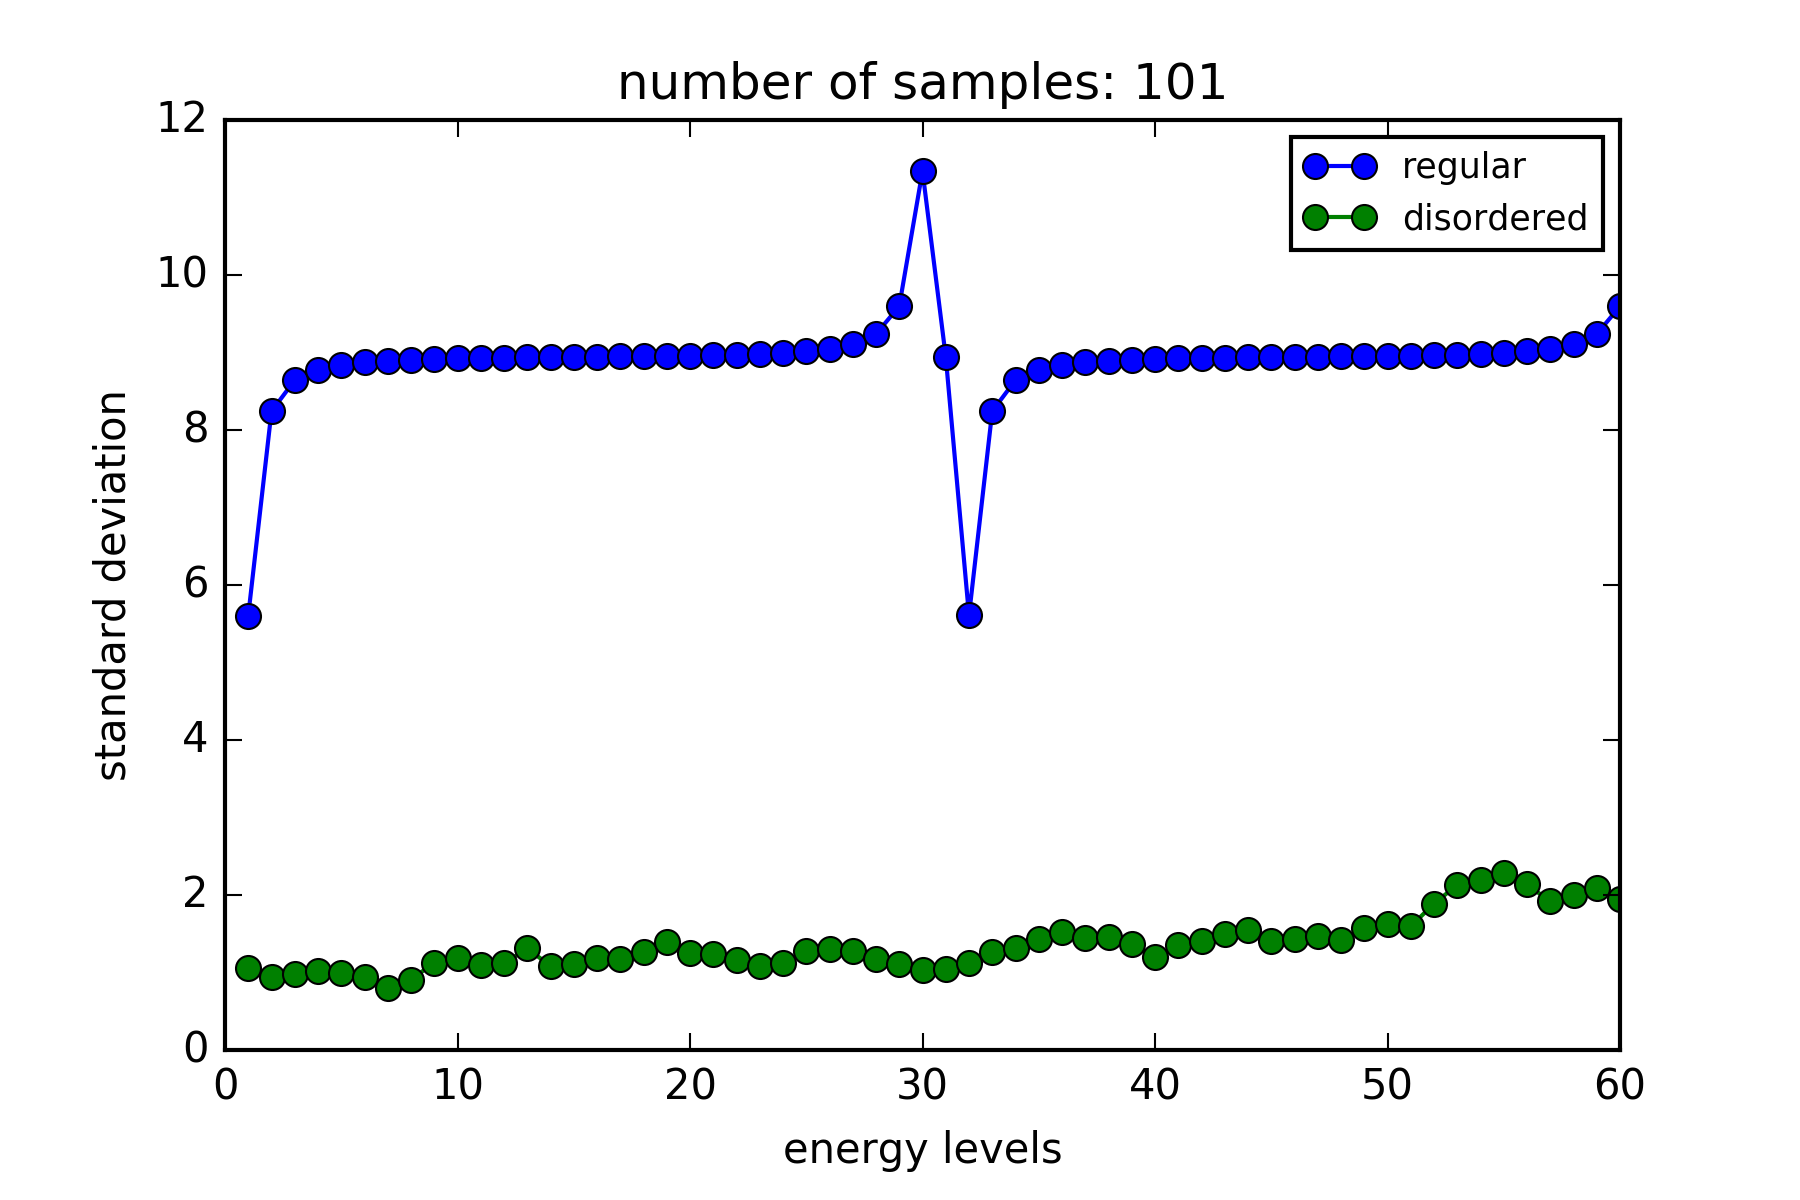
\includegraphics[width=1.1\linewidth]{standardDeviation/N_31_100a30_well0_2_p_0_5.png}
  \captionof{figure}{Localization against energy levels, comparison between Regular System and Disordered System No.8}
  \label{fig:disordered sys num 8}
\end{minipage}
\end{figure}

%end figure



\newpage
\section{Localization of normal modes in harmonic chain model}
\subsection{Randomness in atoms' mass}
The following graphs are normal modes for model 3a in which we introduce randomness to the atom mass at each site by the way we mentioned in Chapter \ref{Ch:Background} model 3b. We retain the same notation as in that section, namely $\{M_1,M_2\}$, and $\{P(M_1),P(M_2)\}$.
For better comparison, probability density function is computed by rescaling to the interval $[0,1]$ and then squaring displacements in the normal mode followed by normalization such that the total area under is 1.
The eigenvalue for each normal mode corresponds to the frequency of that normal mode.
The following are figures plotted when $\{M_1,M_2\} = \{1,2\}$ at different normal modes. Note the normal mode is on the left and the corresponding probability density function is on the left.

%0.5,{1,2} ,26th, 76th, N = 103  
\begin{figure}[!htbh]
\centering
\begin{minipage}{.45\textwidth}
  \centering
  \includegraphics[width=1.1\linewidth]{Harmonic_mass_ratio/normal_Prob_0_5N_103m_2p_26th.png}
  \captionof{figure}{ $N = 103 $, $\{P(M_1),P(M_2) \}= \{0.5,0.5\} $, 26th normal mode}
  \label{fig:mass low frequency}
\end{minipage}\qquad
\begin{minipage}{.45\textwidth}
  \centering
  \includegraphics[width=1.1\linewidth]{Harmonic_mass_ratio/densProb_0_5N_103m_2p_26th.png}
  \captionof{figure}{ $N = 103 $, $\{P(M_1),P(M_2) \}= \{0.5,0.5\} $,26th normal mode}
  \label{fig:N103_1_2_26th_density}
\end{minipage}
\end{figure}

%0.5,{1,2} ,26th, 76th, N = 103  
\begin{figure}[!htbh]
\centering
\begin{minipage}{.45\textwidth}
  \centering
  \includegraphics[width=1.1\linewidth]{Harmonic_mass_ratio/normal_Prob_0_5N_103m_2p_76th.png}
  \captionof{figure}{ $N = 103 $, $\{P(M_1),P(M_2) \}= \{0.5,0.5\} $, 76th normal mode}
  \label{fig:mass high frequency}
\end{minipage}\qquad
\begin{minipage}{.45\textwidth}
  \centering
  \includegraphics[width=1.1\linewidth]{Harmonic_mass_ratio/densProb_0_5N_103m_2p_76th.png}
  \captionof{figure}{ $N = 103 $, $\{P(M_1),P(M_2) \}= \{0.5,0.5\} $,76th normal mode}
  \label{fig:N103_1_2_76th_density}
\end{minipage}
\end{figure}


The following figures are for systems with different number of atoms. Only probability density functions are plotted for comparison. $\{M_1.M_2\} = \{1,2\}$.  

Since the number of normal modes is different for chains of different number of atoms. We choose a third largest frequency for comparison. That is to say for 31 atoms, we choose 28th normal mode while for 61 atoms, we choose 58th normal mode.
% N = 11, 31 ,61 , 101 

\begin{figure}[!htbh]
\centering
\begin{minipage}{.45\textwidth}
  \centering
  \includegraphics[width=1.1\linewidth]{Harmonic_mass_ratio/densProb_0_5N_31m_2p_28th.png}
  \captionof{figure}{ $N = 31 $, $\{P(M_1),P(M_2) \}= \{0.5,0.5\} $, 28th normal mode}
  \label{fig:mass length31 28th}
\end{minipage}\qquad
\begin{minipage}{.45\textwidth}
  \centering
  \includegraphics[width=1.1\linewidth]{Harmonic_mass_ratio/densProb_0_5N_61m_2p_58th.png}
  \captionof{figure}{ $N = 61 $, $\{P(M_1),P(M_2) \}= \{0.5,0.5\} $,58th normal mode}
  \label{fig:mass length61 58th}
\end{minipage}
\end{figure}


%101 ,201
\begin{figure}[!htbh]
\centering
\begin{minipage}{.45\textwidth}
  \centering
  \includegraphics[width=1.1\linewidth]{Harmonic_mass_ratio/densProb_0_5N_101m_2p_98th.png}
  \captionof{figure}{ $N = 101$, $\{P(M_1),P(M_2) \}= \{0.5,0.5\} $, 98th normal mode}
  \label{fig:mass length101 98th}
\end{minipage}\qquad
\begin{minipage}{.45\textwidth}
  \centering
  \includegraphics[width=1.1\linewidth]{Harmonic_mass_ratio/densProb_0_5N_201m_2p_198th.png}
  \captionof{figure}{$N = 201$, $\{P(M_1),P(M_2) \}= \{0.5,0.5\} $, 198th normal mode}
  \label{fig:mass length201 198th}
\end{minipage}
\end{figure}

\newpage
The following are figures for systems with the same number of atoms,same randomness($\{P(M_1),P(M_2) \}= \{0.5,0.5\} $), but different $\{M_1, M_2\}$. Here, we only vary $M_2$, $M_1$ is fixed to be 1. 

% N = 31, 61, 101, 201 




% M = 1.1,1.5,2.0,10.0,20.0,40.0
\begin{figure}[!htbh]
\centering
\begin{minipage}{.45\textwidth}
  \centering
  \includegraphics[width=1.1\linewidth]{Harmonic_mass_ratio/normal_Prob_0_5N_103m_1_1p_51th.png}
  \captionof{figure}{ $N = 103$, $\{M_1,M_2\} = \{1,1.1\}$, 51st normal mode}
  \label{fig:mass ratio 1.1 51st}
\end{minipage}\qquad
\begin{minipage}{.45\textwidth}
  \centering
  \includegraphics[width=1.1\linewidth]{Harmonic_mass_ratio/normal_Prob_0_5N_103m_1_5p_51th.png}
  \captionof{figure}{$N = 103$, $\{M_1,M_2\} = \{1,1.5\}$, 51st normal mode}
  \label{fig:mass ratio 1.5 51st}
\end{minipage}
\end{figure}

%2,10
\begin{figure}[!htbh]
\centering
\begin{minipage}{.45\textwidth}
  \centering
  \includegraphics[width=1.1\linewidth]{Harmonic_mass_ratio/normal_Prob_0_5N_103m_2_0p_51th.png}
  \captionof{figure}{ $N = 103$, $\{M_1,M_2\} = \{1,2\}$, 51st normal mode}
  \label{fig:mass ratio 2.0 51st}
\end{minipage}\qquad
\begin{minipage}{.45\textwidth}
  \centering
  \includegraphics[width=1.1\linewidth]{Harmonic_mass_ratio/normal_Prob_0_5N_103m_10_0p_51th.png}
  \captionof{figure}{$N = 103$, $\{M_1,M_2\} = \{1,10\}$, 51st normal mode}
  \label{fig:mass ratio 10.0 51st}
\end{minipage}
\end{figure}

%20, 40 

\begin{figure}[!htbh]
\centering
\begin{minipage}{.45\textwidth}
  \centering
  \includegraphics[width=1.1\linewidth]{Harmonic_mass_ratio/normal_Prob_0_5N_103m_20_0p_51th.png}
  \captionof{figure}{ $N = 51$, $\{M_1,M_2\} = \{1,20\}$, 51st normal mode}
  \label{fig:mass ratio 20.0 51st}
\end{minipage}\qquad
\begin{minipage}{.45\textwidth}
  \centering
  \includegraphics[width=1.1\linewidth]{Harmonic_mass_ratio/normal_Prob_0_5N_103m_40_0p_51th.png}
  \captionof{figure}{$N = 51$, $\{M_1,M_2\} = \{1,40\}$, 41th normal mode}
  \label{fig:mass ratio 40.0 51st}
\end{minipage}
\end{figure}

\newpage
The following are figures for systems with the same number of atoms,same $\{M_1, M_2\}$, but different $\{P(M_1), P(M_2)\}$. Here, we compare 2 different probabilities, namely $\{0.1, 0.9\}$ and $\{0.5, 0.5\}$. 

%26th
\begin{figure}[!htbh]
\centering
\begin{minipage}{.45\textwidth}
  \centering
  \includegraphics[width=1.1\linewidth]{Harmonic_mass_ratio/normal_Prob_0_1N_103m_2p_26th.png}
  \captionof{figure}{ $N = 103$, $\{P(M_1), P(M_2)\}= \{0.1,0.9\}$ ,$\{M_1,M_2\} = \{1,2\}$, 26th normal mode}
  \label{fig:mass prob 0.1 26th}
\end{minipage}\qquad
\begin{minipage}{.45\textwidth}
  \centering
  \includegraphics[width=1.1\linewidth]{Harmonic_mass_ratio/normal_Prob_0_5N_103m_2p_26th.png}
  \captionof{figure}{$N = 103$,$\{P(M_1), P(M_2)\}= \{0.5,0.5\}$ , $\{M_1,M_2\} = \{1,2\}$, 26th normal mode}
  \label{fig:mass prob 0.5 26th}
\end{minipage}
\end{figure}

%51st 
\begin{figure}[!htbh]
\centering
\begin{minipage}{.45\textwidth}
  \centering
  \includegraphics[width=1.1\linewidth]{Harmonic_mass_ratio/normal_Prob_0_1N_103m_2p_51th.png}
  \captionof{figure}{ $N = 103$, $\{P(M_1), P(M_2)\}= \{0.1,0.9\}$ ,$\{M_1,M_2\} = \{1,2\}$, 51st normal mode}
  \label{fig:mass prob 0.1 51th}
\end{minipage}\qquad
\begin{minipage}{.45\textwidth}
  \centering
  \includegraphics[width=1.1\linewidth]{Harmonic_mass_ratio/normal_Prob_0_5N_103m_2p_51th.png}
  \captionof{figure}{$N = 103$,$\{P(M_1), P(M_2)\}= \{0.5,0.5\}$ , $\{M_1,M_2\} = \{1,2\}$, 51st normal mode}
  \label{fig:mass prob 0.5 51th}
\end{minipage}
\end{figure}


%76th
\begin{figure}[!htbh]
\centering
\begin{minipage}{.45\textwidth}
  \centering
  \includegraphics[width=1.1\linewidth]{Harmonic_mass_ratio/normal_Prob_0_1N_103m_2p_76th.png}
  \captionof{figure}{ $N = 103$, $\{P(M_1), P(M_2)\}= \{0.1,0.9\}$ ,$\{M_1,M_2\} = \{1,2\}$, 76th normal mode}
  \label{fig:mass prob 0.1 76th}
\end{minipage}\qquad
\begin{minipage}{.45\textwidth}
  \centering
  \includegraphics[width=1.1\linewidth]{Harmonic_mass_ratio/normal_Prob_0_5N_103m_2p_76th.png}
  \captionof{figure}{$N = 103$,$\{P(M_1), P(M_2)\}= \{0.5,0.5\}$ , $\{M_1,M_2\} = \{1,2\}$, 76th normal mode}
  \label{fig:mass prob 0.5 76th}
\end{minipage}
\end{figure}

%101st
\begin{figure}[!htbh]
\centering
\begin{minipage}{.45\textwidth}
  \centering
  \includegraphics[width=1.1\linewidth]{Harmonic_mass_ratio/normal_Prob_0_1N_103m_2p_101th.png}
  \captionof{figure}{ $N = 103$, $\{P(M_1), P(M_2)\}= \{0.1,0.9\}$ ,$\{M_1,M_2\} = \{1,2\}$, 101st normal mode}
  \label{fig:mass prob 0.1 101th}
\end{minipage}\qquad
\begin{minipage}{.45\textwidth}
  \centering
  \includegraphics[width=1.1\linewidth]{Harmonic_mass_ratio/normal_Prob_0_5N_103m_2p_101th.png}
  \captionof{figure}{$N = 103$,$\{P(M_1), P(M_2)\}= \{0.5,0.5\}$ , $\{M_1,M_2\} = \{1,2\}$, 101st normal mode}
  \label{fig:mass prob 0.5 101th}
\end{minipage}
\end{figure}


\newpage
\subsection{Randomness in harmonic strings' elastic constant}
The following graphs are normal modes for model 3b in which we introduce randomness to the harmonic strings' elastic constant by the way we mentioned in section \ref{Ch:Background} model 3c. We retain the same notation as in that section, namely $\{K_1,K_2\}$, and $\{P(K_1),P(K_2)\}$. 
For better comparison between chains of different number of atoms, probability density function is sometimes computed by rescaling to the interval $[0,1]$ and then squaring displacements in the normal mode followed by normalization such that the total area under is 1.


The following are figures plotted when $\{K_1,K_2\} = \{1,2\}$ at different normal modes. Note the normal mode is on the left and the corresponding probability density function is on the left.

%spring constant ratio: 0.5,{1,2} ,26th, 76th, N = 103  
\begin{figure}[!htbh]
\centering
\begin{minipage}{.45\textwidth}
  \centering
  \includegraphics[width=1.1\linewidth]{Harmonic_spring_ratio/spr_N_103sp_2p_0_526th.png}
  \captionof{figure}{ $N = 103 $, $\{P(M_1),P(M_2) \}= \{0.5,0.5\} $, 26th normal mode}
  \label{fig:spring normal mode low frequency}
\end{minipage}\qquad
\begin{minipage}{.45\textwidth}
  \centering
  \includegraphics[width=1.1\linewidth]{Harmonic_spring_ratio/densProb_0_5N_103m_2p_26th.png}
  \captionof{figure}{ $N = 103 $, $\{P(M_1),P(M_2) \}= \{0.5,0.5\} $,26th normal mode}
  \label{fig:spring prob density low frequency}
\end{minipage}
\end{figure}

%56th 
\begin{figure}[!htbh]
\centering
\begin{minipage}{.45\textwidth}
  \centering
  \includegraphics[width=1.1\linewidth]{Harmonic_spring_ratio/spr_N_103sp_2p_0_551th.png}
  \captionof{figure}{ $N = 103 $, $\{P(M_1),P(M_2) \}= \{0.5,0.5\} $, 51st normal mode}
  \label{fig:spring normal mode mid range frequency}
\end{minipage}\qquad
\begin{minipage}{.45\textwidth}
  \centering
  \includegraphics[width=1.1\linewidth]{Harmonic_spring_ratio/densProb_0_5N_103m_2p_51th.png}
  \captionof{figure}{ $N = 103 $, $\{P(M_1),P(M_2) \}= \{0.5,0.5\} $,51st normal mode}
  \label{fig:spring prob density mid range frequency}
\end{minipage}
\end{figure}

%76th 
\begin{figure}[!htbh]
\centering
\begin{minipage}{.45\textwidth}
  \centering
  \includegraphics[width=1.1\linewidth]{Harmonic_spring_ratio/spr_N_103sp_2p_0_576th.png}
  \captionof{figure}{ $N = 103 $, $\{P(M_1),P(M_2) \}= \{0.5,0.5\} $, 76th normal mode}
  \label{fig:spring normal mode high frequency}
\end{minipage}\qquad
\begin{minipage}{.45\textwidth}
  \centering
  \includegraphics[width=1.1\linewidth]{Harmonic_spring_ratio/densProb_0_5N_103m_2p_76th.png}
  \captionof{figure}{ $N = 103 $, $\{P(M_1),P(M_2) \}= \{0.5,0.5\} $,76th normal mode}
  \label{fig:spring prob density high frequency}
\end{minipage}
\end{figure}


%2 
\newpage
The following figures are for systems with different number of atoms. Only probability density functions are plotted for comparison. 

%spring N = 31, 61 
\begin{figure}[!htbh]
\centering
\begin{minipage}{.45\textwidth}
  \centering
  \includegraphics[width=1.1\linewidth]{Harmonic_spring_ratio/densProb_0_5N_31m_2p_28th.png}
  \captionof{figure}{ $N = 31 $, $\{P(K_1),P(K_2) \}= \{0.5,0.5\} $, 28th normal mode}
  \label{fig:spring_N_31m_2_28th}
\end{minipage}\qquad
\begin{minipage}{.45\textwidth}
  \centering
  \includegraphics[width=1.1\linewidth]{Harmonic_spring_ratio/densProb_0_5N_61m_2p_58th.png}
  \captionof{figure}{ $N = 61 $, $\{P(K_1),P(K_2) \}= \{0.5,0.5\} $,58th normal mode}
  \label{fig:spring_N_61m_2_58th}
\end{minipage}
\end{figure}


%101 ,201
\begin{figure}[!htbh]
\centering
\begin{minipage}{.45\textwidth}
  \centering
  \includegraphics[width=1.1\linewidth]{Harmonic_spring_ratio/densProb_0_5N_101m_2p_98th.png}
  \captionof{figure}{ $N = 101$, $\{P(K_1),P(K_2) \}= \{0.5,0.5\} $, 98th normal mode}
  \label{fig:spring_N_101m_2_98th}
\end{minipage}\qquad
\begin{minipage}{.45\textwidth}
  \centering
  \includegraphics[width=1.1\linewidth]{Harmonic_spring_ratio/densProb_0_5N_201m_2p_198th.png}
  \captionof{figure}{$N = 201$, $\{P(K_1),P(K_2) \}= \{0.5,0.5\} $, 198th normal mode}
  \label{fig:spring_N_201m_2_198th}
\end{minipage}
\end{figure}


%3
\newpage
The following are figures for systems with the same number of atoms,same randomness($\{P(K_1),P(K_2) \}= \{0.5,0.5\} $), but different $\{K_1, K_2\}$. Here, we only vary $K_2$. $K_1$ is fixed to be 1. 



% K_2 = 1.1,1.5,2.0,10.0,20.0,40.0
\begin{figure}[!htbh]
\centering
\begin{minipage}{.45\textwidth}
  \centering
  \includegraphics[width=1.1\linewidth]{Harmonic_spring_ratio/spr_N_103sp_1_1p_0_576th.png}
  \captionof{figure}{ $N = 103$, $\{K_1,K_2\} = \{1,1.1\}$, 76th normal mode}
  \label{fig:spring_N_103m_1.1_p_0_5_76th}
\end{minipage}\qquad
\begin{minipage}{.45\textwidth}
  \centering
  \includegraphics[width=1.1\linewidth]{Harmonic_spring_ratio/spr_N_103sp_1_5p_0_576th.png}
  \captionof{figure}{$N = 103$, $\{K_1,K_2\} = \{1,1.5\}$, 76th normal mode}
  \label{fig:spring_N_103m_1.5_p_0_5_51st}
\end{minipage}
\end{figure}
%2, 5 
\begin{figure}[!htbh]
\centering
\begin{minipage}{.45\textwidth}
  \centering
  \includegraphics[width=1.1\linewidth]{Harmonic_spring_ratio/spr_N_103sp_2_0p_0_576th.png}
  \captionof{figure}{ $N = 103$, $\{K_1,K_2\} = \{1,2\}$, 76th normal mode}
  \label{fig:spring_N_103m_2.0_p_0_5_76th}
\end{minipage}\qquad
\begin{minipage}{.45\textwidth}
  \centering
  \includegraphics[width=1.1\linewidth]{Harmonic_spring_ratio/spr_N_103sp_5_0p_0_576th.png}
  \captionof{figure}{$N = 103$, $\{K_1,K_2\} = \{1,5\}$, 76th normal mode}
  \label{fig:spring_N_103m_5.0_p_0_5_51st}
\end{minipage}
\end{figure}

%10, 20
\begin{figure}[!htbh]
\centering
\begin{minipage}{.45\textwidth}
  \centering
  \includegraphics[width=1.1\linewidth]{Harmonic_spring_ratio/spr_N_103sp_10_0p_0_576th.png}
  \captionof{figure}{ $N = 103$, $\{K_1,K_2\} = \{1,10\}$, 76th normal mode}
  \label{fig:spring_N_103m_10.0_p_0_5_76th}
\end{minipage}\qquad
\begin{minipage}{.45\textwidth}
  \centering
  \includegraphics[width=1.1\linewidth]{Harmonic_spring_ratio/spr_N_103sp_20_0p_0_576th.png}
  \captionof{figure}{$N = 103$, $\{K_1,K_2\} = \{1,20\}$, 76th normal mode}
  \label{fig:spring_N_103m_20.0_p_0_5_51st}
\end{minipage}
\end{figure}

\newpage
The following are figures for systems with the same number of atoms,same $\{K_1, K_2\}$, but different $\{P(K_1), P(K_2)\}$. Here, we compare 2 different probabilities, namely $\{0.1, 0.9\}$ and $\{0.5, 0.5\}$. 

%26th
\begin{figure}[!htbh]
\centering
\begin{minipage}{.45\textwidth}
  \centering
  \includegraphics[width=1.1\linewidth]{Harmonic_spring_ratio/prob_spr_N_103sp_2_0p_0_126th.png}
  \captionof{figure}{ $N = 103$, $\{P(K_1), P(K_2)\}= \{0.1,0.9\}$ ,$\{K_1,K_2\} = \{1,2\}$, 26th normal mode}
  \label{fig:prob_spring_N_103m_2p_0_1_26th}
\end{minipage}\qquad
\begin{minipage}{.45\textwidth}
  \centering
  \includegraphics[width=1.1\linewidth]{Harmonic_spring_ratio/prob_spr_N_103sp_2_0p_0_526th.png}
  \captionof{figure}{$N = 103$,$\{P(K_1), P(K_2)\}= \{0.5,0.5\}$ , $\{K_1,K_2\} = \{1,2\}$, 26th normal mode}
  \label{fig:prob_spring_N_103m_2p_0_5_26th}
\end{minipage}
\end{figure}

%51st
\begin{figure}[!htbh]
\centering
\begin{minipage}{.45\textwidth}
  \centering
  \includegraphics[width=1.1\linewidth]{Harmonic_spring_ratio/prob_spr_N_103sp_2_0p_0_151th.png}
  \captionof{figure}{ $N = 103$, $\{P(K_1), P(K_2)\}= \{0.1,0.9\}$ ,$\{K_1,K_2\} = \{1,2\}$, 51st normal mode}
  \label{fig:prob_spring_N_103m_2p_0_1_51st}
\end{minipage}\qquad
\begin{minipage}{.45\textwidth}
  \centering
  \includegraphics[width=1.1\linewidth]{Harmonic_spring_ratio/prob_spr_N_103sp_2_0p_0_551th.png}
  \captionof{figure}{$N = 103$,$\{P(K_1), P(K_2)\}= \{0.5,0.5\}$ , $\{K_1,K_2\} = \{1,2\}$, 51st normal mode}
  \label{fig:prob_spring_N_103m_2p_0_5_51st}
\end{minipage}
\end{figure}

%76th
\begin{figure}[!htbh]
\centering
\begin{minipage}{.45\textwidth}
  \centering
  \includegraphics[width=1.1\linewidth]{Harmonic_spring_ratio/prob_spr_N_103sp_2_0p_0_176th.png}
  \captionof{figure}{ $N = 103$, $\{P(K_1), P(K_2)\}= \{0.1,0.9\}$ ,$\{K_1,K_2\} = \{1,2\}$, 76th normal mode}
  \label{fig:prob_spring_N_103m_2p_0_1_76th}
\end{minipage}\qquad
\begin{minipage}{.45\textwidth}
  \centering
  \includegraphics[width=1.1\linewidth]{Harmonic_spring_ratio/prob_spr_N_103sp_2_0p_0_576th.png}
  \captionof{figure}{$N = 103$,$\{P(K_1), P(K_2)\}= \{0.5,0.5\}$ , $\{K_1,K_2\} = \{1,2\}$, 76th normal mode}
  \label{fig:prob_spring_N_103m_2p_0_5_76th}
\end{minipage}
\end{figure}

%101st
\begin{figure}[!htbh]
\centering
\begin{minipage}{.45\textwidth}
  \centering
  \includegraphics[width=1.1\linewidth]{Harmonic_spring_ratio/prob_spr_N_103sp_2_0p_0_1101th.png}
  \captionof{figure}{ $N = 103$, $\{P(K_1), P(K_2)\}= \{0.1,0.9\}$ ,$\{K_1,K_2\} = \{1,2\}$, 101st normal mode}
  \label{fig:prob_spring_N_103m_2p_0_1_101st}
\end{minipage}\qquad
\begin{minipage}{.45\textwidth}
  \centering
  \includegraphics[width=1.1\linewidth]{Harmonic_spring_ratio/prob_spr_N_103sp_2_0p_0_5101th.png}
  \captionof{figure}{$N = 103$,$\{P(K_1), P(K_2)\}= \{0.5,0.5\}$ , $\{K_1,K_2\} = \{1,2\}$, 101st normal mode}
  \label{fig:prob_spring_N_103m_2p_0_5_101st}
\end{minipage}
\end{figure}


\endinput

% Chapter 5
\ifthenelse{\boolean{@twoside}}{\myclearpage}{}
\chapter{Discussion}\label{Ch:Discussion}



\section{Band Gaps in Kronig Penney Model}

The band gap increases when the potential height increases at a fixed well width as we can see from Figure \ref{fig: band gap against potential }. This matches with our intuition that when the electron is trapped in deeper wells, it leads to a larger band gap. 

However, when fixing the potential, we see that the band gap increases and then decreases as well width increases, resulting in a peak in Figure \ref{fig:band gap against well width fixed potential}. Intuitively, the peak could be understood by considering two extreme cases, namely when the well width very small and when the well width is as wide as possible. In the first case, there is almost no potential, hence no band gap. In the latter case, the whole system has a negative constant potential along the x-axis, so the band gap vanishes. It is more interesting to see that the peak point move towards the left as we increase the potential height, $V_0$. 


\section{Localization in random Kronig Penney Model}
\subsubsection{Factors affecting localization}\label{subsub:Factors affecting localization}
From the figures in Section \ref{sec: localization}, we see that in both disordered system, one with randomness in atomic spacing and the other with randomness in potential, localization of the probability density function can be observed. Since the probability function is derived by squaring the eigenstate, or in other word, the wave function. We can deduce that the eigenstates are also localized in certain regions. In fact, the figures for probability density function corresponding to higher energy also show the same feature, but we only presented several figures for the lowest energies due to space limit. Hence, we infer that localization of eigenstates is a general property for disorder one dimensional systems subject to certain randomness, more specifically , randomness in atomic spacing and atomic potential.

Here, for convenience, before introducing a measure for degree of localization, we say that the eigenstate has a higher degree of localization if the probability density function is less wider and has a higher peak. So we need to check both the x-coordinate for the localization region and the y coordinate for localization peak. It is interesting to see that the degree of localization is affected by the area of the square potential($V_0l$).Through comparing Figure \ref{fig:Area1_1thlowestRand0.8} - \ref{fig:Area1_1thlowestRand1.5} with Figure \ref{fig:Area10_1thlowestRand0.8} - \ref{fig:Area10_1thlowestRand1.5}, we can see that the probability density function is more localized and has a much higher peak in Figure \ref{fig:Area10_1thlowestRand0.8} - \ref{fig:Area10_1thlowestRand1.5} with $V_0l = 10$ than in Figure \ref{fig:Area1_1thlowestRand0.8} - \ref{fig:Area1_1thlowestRand1.5} with $V_0l = 1.0$. This is more obvious when we compare Figure  \ref{fig:randPoa1_1th_0.5_0.4} with Figure \ref{fig:randPoa10_1th_0.5_0.4}. Hence, we infer that with all other conditions fixed, the larger the area of the square potential, the more localization there is. More accurately, since the well width is fixed in these cases, it is equivalent to say that with all other conditions fixed, the higher the potential height, the more localization there is. 

We can also see that localization is affected by how much the disordered system is perturbed away from the ordered system. For convenience, we call it magnitude of perturbation. When the disordered system is perturbed away from the ordered system more, i.e. when the magnitude of perturbation is larger,  there is more localization in the probability density function. This can be observed by comparing Figure \ref{fig:Area1_1thlowestRand0.9} and \ref{fig:Area1_1thlowestRand1.5}, Figure \ref{fig:randPoa5_1th_0.5_0.4} and Figure \ref{fig:randPoa5_1th_0.5_0.2}, Figure \ref{fig:randPoa5_2th_0.5_0.4} and Figure \ref{fig:randPoa5_2th_0.5_0.2}. 

\subsubsection{Floating point number precision problem}
Floating point precision, in learning or simulating systems with localization property should be taken into account and payed extra attention to. We call the problem  a precision problem, that means due to lack of consideration about precision, an error or noise is introduced to a system and leads to biased or wrong results. In our case, the precision problem causes each square well potential to shift from the atom site by 0, 1 or 2 grid points, introducing some randomness to the periodic system, so when the well width is small, the randomness becomes significant enough. This can be seen from Figure \ref{fig:oldPo_0.4} and Figure \ref{fig:oldPo_0.3}, where the probability density functions are localized but both are regular system. After fixing the problem, the probability density function become normal as shown in Figure \ref{fig:newPo_0.3} and Figure \ref{fig:newPo_0.4}. But it is noticeable  in Figure \ref{fig:oldPo_0.5} and Figure \ref{fig:newPo_0.5} that there is no localization for the probability density functions before and after taking precision problem into account. This might be that the well width is big enough so that the precision problem does not dominate. 
\subsubsection{A measure for degree of localization
}
Standard deviations computed from the probability density function are used to describe how much an eigenstate is localized. A smaller standard deviation indicate a more localized eigenstate while a larger standard deviation means that the eigenstate is less localized. The figures presented in Chapter \ref{Ch:Results} show different localization properties for eigenstates at different energy levels. 
Overall, localization properties mentioned in “Factors affecting localization” is well depicted after using standard deviation as a measure. More specifically, the effect of potential height and magnitude of perturbation on degree of localization that has been illustrated in the preceding subsection are better shown in the figures with standard deviation drawn against energy levels. 
If we disregard the eigenstates for energy levels greater than 30, and comparing disordered system No.1 (See Figure \ref{fig:disordered sys num 1}) with disordered No.2 (See Figure \ref{fig:disordered sys num 2}), disordered system No.3 (See Figure \ref{fig:disordered sys num 3}) with No.4 (See Figure \ref{fig:disordered sys num 4}), we can see that disordered systems that are more perturbed from the ordered system indeed have more localized eigenstates from the fact that the standard deviations for those probability density functions are smaller.  
If we compare disordered system No.1 (Figure \ref{fig:disordered sys num 1}) with No.3 (Figure \ref{fig:disordered sys num 3}), the latter has smaller standard deviations for its probability density function, indicating that a larger potential height leads to more localizations for eigenstates. Similar comparisons can be made between disorders system No.2(Figure \ref{fig:disordered sys num 2}) and No.4(Figure \ref{fig:disordered sys num 4}), No.5(Figure \ref{fig:disordered sys num 5}) and No.7(Figure \ref{fig:disordered sys num 7}), No.6(Figure \ref{fig:disordered sys num 6}) and No.8(Figure \ref{fig:disordered sys num 8}). However, the pattern is not so obvious for comparison between disordered system No.6 and No.8, an reasonable explanation would be that the eigenstates are already very localized so that further changing the potential height or magnitude of perturbation do not contribute much to its localization. (We will see similar property in the next section on harmonic chain models.)
Moreover, it can be observed for disordered systems with randomness in atomic spacing that the degree of localization is different for eigenstates at different energy levels. More interestingly, for the eigenstates corresponding to the first 31 energy levels, a peak is observed on the curve in the middle of the first 31 energy levels. This implies that the eigenstates is more localized as the energy level approaches 1 or 31. Though we are not sure why this happens, it would be useful to understand why the these eigenstates have less localization than others because it may reveal some differences between different energy levels. However, such a pattern does not occur in disordered systems with randomness in potential(disordered system No.5 - No.8) as the curve is relatively flat, showing similar amount of localization for the first 31 eigenstates.  



\section{Localization of normal modes}
\subsubsection{randomness in mass ratio}

For a harmonic chain of atoms with two different masses, $M_1$ and $M_2$, we explore different factors that affect the localization of normal modes. Several results are summarized as below: 
We observe that there is more localization for normal modes at high frequency range than at low frequency range. This can be seen from Figure \ref{fig:mass low frequency} and Figure \ref{fig:mass high frequency} in which the 76th normal mode is more localized than the 26th. 

With the same probability distribution for the two masses, we examine a chain of different number of atoms, and the result shows that more localization is observed with a longer chain if we look at a particular frequency. The comparison is made between a chain of 31, 61,101, and 201 atoms(See Figure \ref{fig:mass length31 28th} to Figure \ref{fig:mass length201 198th}).Note that probability density functions are computed from the normal modes for comparison in this case.

Effect of different masses ratios on the degree of localization is also explored, with results showing that given the same arrangement of atoms with mass $M_1$ or $M_2$, the localization increases as the mass ratio $M_2/M_1$ increases. In our result, we look at the 51st normal mode as a representative and we can see that increase in localization is dramatic when the mass ratio changes from $1$ to $10$, but further increase in mass ratio from $10$ to $40$ does not contribute much to localization. The localization stabilizes at certain mass ratio(See Figure \ref{fig:mass ratio 1.1 51st} to Figure \ref{fig:mass ratio 40.0 51st}). This relation is important as it reveals that in order to achieve a certain degree of localization, it is not necessary to require the mass ratio to be too large. Once the mass ratio reaches a threshold value, no significant change in localization will be seen. But we should be careful that this threshold may vary depending on other factors, e.g. length of the chain, frequency of the normal mode, etc. 

Two different probability distributions for masses, namely $\{0.5,0.5\}$ and $\{0.1,0.9\}$ are compared, with $\{0.5,0.5\}$  showing more localization if we fix a frequency of normal mode(See Figure \ref{fig:mass prob 0.1 26th} to Figure \ref{fig:mass prob 0.5 101th}). To some extent, this indicate that a more disordered system displays more localization in normal modes, since around half of the atoms are of different masses with probability distribution $\{0.5, 0.5\}$ while only about one tenth of the atoms are of different mass with $\{0.1, 0.9\}$. The latter is clearly less disordered. 

\subsubsection{randomness in elastic constant}

Similarly, for a harmonic chain of atoms with two different elastic constants, $K_1$ and $K_2$, we also explore different factors that affect the localization of normal modes. The results are similar to that of randomness in masses and are summarized as below. 
Under a same probability distribution for the elastic constants: 
\begin{itemize}
\item 
More localization is observed at normal modes with higher frequencies. (See Figure \ref{fig:spring normal mode low frequency} to Figure \ref{fig:spring prob density high frequency})
\item
Longer chain of atoms tend to have more localization in their normal modes.
\item
Given an arrangement of atoms with two elastic constant choices $K_1$, $K_2$, increasing the elastic constant ratio ($K_2/K_1$) increases the localization for the normal mode. However, once the ratio is above a certain threshold value, the localization pattern stabilizes and become no longer sensitive to change in this ratio. 
\end{itemize}

With two different probability distributions, namely $\{0.5,0.5\}$ and $\{0.1,0.9\}$, there is more localization with  $\{0.5,0.5\}$. Again, this might imply that more disordered system have more localization in their normal modes. 


\section{Future work}

Although some interesting results have been obtained from our numerical experiments, some other properties can be further explored in more details with the methodology provided in this paper. Below is a summary of several interesting things that we do not have time to experiment with, but readers are encouraged to explore them.
\subsubsection{Band gap}
Non-overlapping potentials of different shapes can be applied to see what band structure it gives. One can also compute the band gap for such potential to see if there is any relation if we modify the potential in a certain way.

Overlapping potentials that take surrounding atoms into account can also be explored to see if the band structure differs from that for non-overlapping potentials. In fact, the result for this case will be more practical because in reality each neighboring atom is interacting with the electron. 

Band structure of a chain of identical super cells in which each cell contains several atoms can be plotted using the same method. Band gap can also be computed for this chain of super cells. Modifying the structure of super cell allows us to see how different atom compositions of a super cell affect the band gap. 

\subsubsection{Localization of eigenstates}
In this paper, we explore randomness in potential with modification based on only square potential wells. Other potentials can be tried using our method to see if localization is indeed a universal property for random systems. Comparisons can be made to see if the localization differs with different potentials. 

A more detailed and specific experiment can be done in which we only modify atoms at positions we are interested in to see its localization behavior, instead of generating a random sequence of atoms using a probability distribution. In this way, we have fixed the positions so we can then modify several factors, e.g. potential height, atomic spacings, well width to see their effect on localization. 

Our measure for degree of localization captures several important localization properties, but it is still a quite rough estimate. It is a good idea to explore if there is a better measure for degree of localization, which might reveal localization properties more universally. 

\subsubsection{Proof}

We should try to understand the results that we have mentioned in the discussion analytically by providing a rigorous mathematical proof. For example, for band gap, we should not be satisfied with the intuitive explanation for the occurrence of the peak in Figure \ref{fig:band gap against well width fixed potential}. Also, the results show that more localization occurs when the potential well is deeper. We should also come up with a proof for that. 

\endinput


% Chapter 6
\ifthenelse{\boolean{@twoside}}{\myclearpage}{}
\include{chapter6}

% Chapter 7
\ifthenelse{\boolean{@twoside}}{\myclearpage}{}
\include{chapter7}

% Chapter 8 -- the Conclusion
\ifthenelse{\boolean{@twoside}}{\myclearpage}{}
\include{chapter8}

% Insert text in Table of Contents to highlight the appendix(es)
\addtocontents {toc}{\protect \contentsline {chapter}{APPENDIXES}{}}
\appendix
\ifthenelse{\boolean{@twoside}}{\myclearpage}{}
\input{appendixA}


% Add your bibliography to Contents
\ifthenelse{\boolean{@twoside}}{\myclearpage}{\newpage}
\addtocontents {toc}{\protect \contentsline {chapter}{REFERENCES}{}}
\addcontentsline{toc}{chapter}{Selected Bibliography Including Cited Works}  % Use the 'bibname' name here.  See below.

% Bibliography must come last.
\bibliographystyle{siam}     % Siam and Ieeetr bibliographic styles treat titles of articles in journals or collections correctly
\renewcommand\bibname{Selected Bibliography Including Cited Works}
\nocite{*}  % List ALL references in your references, not just the ones cited in the text.
% This scheme automatically alphabetizes the Bibliography.
\bibliography{AA-Bibliography/Biblio}

\end{document}
